\documentclass[9pt,twocolumn]{scrartcl}

%\documentclass[9pt]{sigcomm-alternate}

%\usepackage[margin=1in,bottom=1.2in]{geometry}
\usepackage{amsfonts,amssymb,amsmath}
\usepackage[thmmarks,hyperref,amsthm,amsmath]{ntheorem}
\usepackage{graphicx}
\usepackage[ruled,vlined,commentsnumbered]{algorithm2e}
\usepackage[usenames,dvipsnames]{color}
\usepackage{hyperref}
\usepackage{multirow}
\usepackage{lineno}
\usepackage[shortlabels]{enumitem}
\usepackage[utf8]{inputenc}
\usepackage[OT4]{fontenc}
\usepackage{comment}
\usepackage{fancyhdr}
\usepackage{tikz}
%Used Symbols
%c_i = chunk i
%v_i = vm i
%b_t = transfer bandwidth
%b_c = pairwise communication bandwidth
%n = |VMs| = |Chunks|


%Header Extensions Seperation
%Carlo
\newcommand{\VmSlot}{\text{VM slot}}
\newcommand{\VmSlots}{\VmSlot\text{s}}
\newcommand{\Capacity}{\ensuremath{\textsc{cap}}}
\newcommand{\VM}{\textsc{VM}}
\newcommand{\Problem}{\textsc{DummyName Problem}}
\newcommand{\carlo}[1]{\textcolor{red}{carlo: #1}}
\newcommand{\maciek}[1]{\textcolor{brown}{maciek: #1}}
\newcommand{\stefan}[1]{\textcolor{blue}{stefan: #1}}
\newcommand{\MaFactor}{r}
\newcommand{\Path}{\ensuremath{p}}
\newcommand{\RedundancyFactor}{\ensuremath{r}}

\newcommand{\variab}{\nu}

\newcommand{\Source}{\ensuremath{s}}
\newcommand{\Sink}{\ensuremath{t}}

\newcommand{\VmChunkAssignment}{\mu}
\newcommand{\NodeMapping}{\pi}
\newcommand{\ChunkLocation}{\pi}

\newcommand{\ChunkType}{\tau}
\newcommand{\VirtualNodes}{\ensuremath{V}}
\newcommand{\VirtualEdges}{\ensuremath{E_V}}
\newcommand{\VirtualNode}{v}
\newcommand{\VirtualEdge}{e}
\newcommand{\VCSwitch}{\ensuremath{\textsc{center}}}
\newcommand{\SubstrateNodes}{\ensuremath{V_S}}
\newcommand{\SubstrateEdges}{\ensuremath{E_S}}
\newcommand{\SubstrateNode}{\ensuremath{v}}
\newcommand{\SubstrateEdge}{\ensuremath{e}}
\newcommand{\Leaf}{\ensuremath{l}}
\newcommand{\Leaves}{\ensuremath{L}}
\newcommand{\Chunks}{\ensuremath{\textsc{chunks}}}
\newcommand{\aroot}{\emph{root}}

\newcommand{\Opt}{\ensuremath{Opt}}
\newcommand{\Children}{\ensuremath{children}}
%\newcommand{\Cost}{\ensuremath{\textsc{cost}}}

\newcommand{\Uplink}{\ensuremath{\textsc{uplink}}}
\newcommand{\ChunkCount}{\ensuremath{\textsc{cis}}}
\newcommand{\VmCount}{\ensuremath{\textsc{vis}}}
\newcommand{\Right}{\ensuremath{r}}
\newcommand{\InverseAssignment}{\ensuremath{\VmChunkAssignment^{-1}}}

\newcommand{\clauses}{\alpha}
\newcommand{\vars}{\beta}
\newcommand{\variables}{\beta}
\newcommand{\achunk}{\ensuremath{c}}
\newcommand{\Chunk}{\ensuremath{c}}
\newcommand{\capa}{\emph{cap}}
\newcommand{\capacity}{\emph{cap}}
\newcommand{\Distance}{\emph{\textsc{dist}}}
\newcommand{\dist}{\emph{dist}}
\newcommand{\CostPerChunk}{\emph{cost}}


\newcommand{\VC}{\textsc{VC}}
\newcommand{\CC}{\textsc{NI}}

\newcommand{\VE}{\textsc{VE}}
\newcommand{\FP}{\textsc{FP}}
\newcommand{\RS}{\textsc{RS}}
\newcommand{\BW}{\textsc{BW}}
\newcommand{\MA}{\textsc{MA}}
\newcommand{\Cost}{\textsc{F}}

\newcommand{\MatchCost}{\textsc{MCost}}
\newcommand{\chunkOf}{\textsc{chunkOf}}


%Maciek

\newcommand{\Bandwidth}{\ensuremath{bw}}
\newcommand{\Tree}{\ensuremath{T}}
\newcommand{\CostTrans}{\ensuremath{b_1}}
\newcommand{\CostCom}{\ensuremath{b_2}}
\newcommand{\Vms}{\ensuremath{n_V}}
\newcommand{\TSC}{\textsc{3-SC}}
\newcommand{\TDM}{\textsc{3-DM}}
\newcommand{\TSAT}{\textsc{3-Sat}}
\newcommand{\NSAT}{\textsc{Sat}}
\newcommand{\SAT}{\textsc{Sat}}
\newcommand{\ZSAT}{\textsc{2-Sat}}


\newcommand{\Formula}{\ensuremath{\Psi}}
\newcommand{\Clauses}{\ensuremath{Cl(\Formula)}}
\newcommand{\NClauses}{\ensuremath{c}}
\newcommand{\Vars}{\ensuremath{Var(\Formula)}}
\newcommand{\NVars}{\ensuremath{|\Vars|}}
\newcommand{\ChunkTypes}{\ensuremath{ch}}
\newcommand{\Thr}{\ensuremath{Th}}
\newcommand{\VCB}{\ensuremath{VCB}}
\newcommand{\VCNB}{\ensuremath{VCNB}}
\newcommand{\varx}{\ensuremath{x}}
\newcommand{\positive}{\ensuremath{positive}}
\newcommand{\negative}{\ensuremath{negative}}
\newcommand{\Val}{\ensuremath{Val}}
\newcommand{\Sol}{\ensuremath{SOL}}



\definecolor{blueLink}{rgb}{0,0.2,0.8}
\hypersetup{colorlinks,linkcolor=blueLink,urlcolor=blueLink,citecolor=blueLink}
\newcommand{\lref}[2][]{\hyperref[#2]{#1~\ref*{#2}}}



%%%%%%%%%%%%%%%%%%%%%%%%%%%%%%%%%%%%%%%%%%%%%%%%%%%%%%%%%%%%%
% GENERAL STYLE MACROS
%%%%%%%%%%%%%%%%%%%%%%%%%%%%%%%%%%%%%%%%%%%%%%%%%%%%%%%%%%%%%

\newcommand{\etal}{{\it et~al.\ }}
\newcommand{\myparagraph}[1]{{\smallskip\noindent{\bf #1}}}
\newcommand{\mycase}[1]{{\underline{Case~#1}:}}

%%%%%%%%%%%%%%%%%%%%%%%%%%%%%%%%%%%%%%%%%%%%%%%%%%%%%%%%%%%%
% THEOREMS AND SUCH
%%%%%%%%%%%%%%%%%%%%%%%%%%%%%%%%%%%%%%%%%%%%%%%%%%%%%%%%%%%%%

\newtheorem{theorem}{Theorem}
\newtheorem{corollary}[theorem]{Corollary}
\newtheorem{lemma}[theorem]{Lemma}
\newtheorem{claim}[theorem]{Claim}
\newtheorem{fact}{Fact}

%%%%%%%%%%%%%%%%%%%%%%%%%%%%%%%%%%%%%%%%%%%%%%%%%%%%%%%%%%%%%
% USEFUL LETTERS
%%%%%%%%%%%%%%%%%%%%%%%%%%%%%%%%%%%%%%%%%%%%%%%%%%%%%%%%%%%%%

\DeclareMathOperator{\polylog}{polylog}
\newcommand{\emdash}{\hspace{1mm}---\hspace{1mm}}
\newcommand{\e}{\mathrm{e}}
\renewcommand{\O}{\mathcal{O}}
\renewcommand{\Pr}{\mathbf{Pr}}
\newcommand{\E}{\mathbf{E}}
\newcommand{\NAT}{\mathbb{N}}
\newcommand{\REAL}{\mathbb{R}}

%%%%%%%%%%%%%%%%%%%%%%%%%%%%%%%%%%%%%%%%%%%%%%%%%%%%%%%%%%%%%
% PARENTHESES ETC
%%%%%%%%%%%%%%%%%%%%%%%%%%%%%%%%%%%%%%%%%%%%%%%%%%%%%%%%%%%%%

\newcommand{\ceiling}[1]{\left\lceil #1 \right\rceil}
\newcommand{\floor}[1]{\left\lfloor #1 \right\rfloor}
\newcommand{\braced}[1]{{\left\{#1\right\}}}
\newcommand{\bigbrackd}[1]{{\big[#1\big]}}
\newcommand{\brackd}[1]{{\left[#1\right]}}
\newcommand{\parend}[1]{{\left(#1\right)}}

%%%%%%%%%%%%%%%%%%%%%%%%%%%%%%%%%%%%%%%%%%%%%%%%%%%%%%%%%%%%%
% FRACTIONS
%%%%%%%%%%%%%%%%%%%%%%%%%%%%%%%%%%%%%%%%%%%%%%%%%%%%%%%%%%%%%

\newcommand{\half}{\frac{1}{2}}
\newcommand{\onehalf}{\frac{1}{2}}
\newcommand{\onethird}{\frac{1}{3}}
\newcommand{\twothirds}{{\textstyle\frac{2}{3}}}
\newcommand{\fourthirds}{{\textstyle\frac{4}{3}}}
\newcommand{\fivethirds}{{\textstyle\frac{5}{3}}}
\newcommand{\threefourths}{{\textstyle\frac{3}{4}}}

%%%%%%%%%%%%%%%%%%%%%%%%%%%%%%%%%%%%%%%%%%%%%%%%%%%%%%%%%%%%%
% ALGORITHM NAMES, ETC
%%%%%%%%%%%%%%%%%%%%%%%%%%%%%%%%%%%%%%%%%%%%%%%%%%%%%%%%%%%%%

\newcommand{\ALG}{\textsc{Alg}}
\newcommand{\OPT}{\textsc{Opt}}
\newcommand{\DET}{\textsc{Det}}
\newcommand{\RAND}{\textsc{Rand}}

%%%%%%%%%%%%%%%%%%%%%%%%%%%%%%%%%%%%%%%%%%%%%%%%%%%%%%%%%%%%%
% PSEUDOCODE
%%%%%%%%%%%%%%%%%%%%%%%%%%%%%%%%%%%%%%%%%%%%%%%%%%%%%%%%%%%%%

\newcommand{\IF}    {{\bf if }}
\newcommand{\THEN}  {{\bf then }} 
\newcommand{\FOR}   {{\bf for }}
\newcommand{\EACH}  {{\bf each }} 
\newcommand{\DO}  {{\bf do }} 

%%%%%%%%%%%%%%%%%%%%%%%%%%%%%%%%%%%%%%%%%%%%%%%%%%%%%%%%%%%%%
% EDITORIAL MACROS
%%%%%%%%%%%%%%%%%%%%%%%%%%%%%%%%%%%%%%%%%%%%%%%%%%%%%%%%%%%%%

\definecolor{brown}{rgb}{0.4,0,0} 
\definecolor{purple}{rgb}{0.2,0,0.6}
\definecolor{hotpink}{rgb}{1,0.4,0.7}
\newcommand{\marginnote}[1]{\marginpar{\scriptsize{\begin{flushleft}#1\end{flushleft}}}}
\newcommand{\todo}[1]{\noindent\colorbox{red}{todo: #1}} 
\newcommand{\marcin}[1]{\color{red} Marcin: #1\color{black}}



\title{A Note on Virtual Cluster Embedding with Data Locality}

\title{Embedding Algorithms for Virtual Clusters with Data Locality and Replica Selection}

\title{Embedding Virtual Clusters with Data Locality and Replica Selection\\{\Large Real Algorithms for Virtual Environments}}

\title{Data Locality and Replica Aware Virtual Cluster Embeddings}
%\\{\Large Real Algorithms for Virtual Environments}}


\author{Carlo Fuerst$^1$, Maciek Pacut$^2$, Stefan Schmid$^3$\\
{\small $^1$ TU Berlin, Germany; $^2$ University of Wroclaw, Poland; $^3$ TU Berlin \& T-Labs, Germany}}

\begin{document}

\maketitle


\begin{abstract}
\textbf{Abstract.} Virtualized datacenters offer great flexibilities in terms of resource allocation. In particular, by
decoupling applications from the constraints of the underlying physical infrastructure, virtualization
supports an optimized mapping of virtual machines as well as their interconnecting network
% (the so-called \emph{virtual cluster})
to their
physical counterparts: essentially a graph embedding problem.

However, existing algorithms
in the literature often ignore a crucial dimension of the embedding problem, namely \emph{data locality}:
the input to a cloud application such as MapReduce is typically stored in a distributed,
and sometimes redundant, file system. Since moving
data is costly, an embedding algorithm should be data locality aware,
and allocate computational resources close to the data; in case of redundant storage, the algorithm should also optimize the \emph{replica selection}.

This paper initiates the algorithmic study of data locality aware virtual cluster embeddings for
the widely used (fat-)tree like datacenter topologies.
In particular, we
show that
despite the multiple degrees of freedom in terms of embedding and replica selection,
many problems can be
solved efficiently, and we highlight interesting connections
to classic optimization problems. However, we also show the limitations of such optimizations,
by presenting several new NP-hardness results; interestingly,
our hardness proofs even hold in uncapacitated settings.
\end{abstract}

\begin{comment}
we should maybe give the main algorithms a name; we should talk about the case where the number of machines is not a perfect multiple;
\end{comment}

%%%%%%%%%%%%%%%%%%%%%%%%%%%%%%%%%%%%%
\section{Introduction}

%Server virtualization has revamped the server business over the last years,
%and has radically changed the way we think about resource allocation:
%today, almost arbitrary computational resources can be allocated on demand.
%Moreover, the virtualization trend now started to spill over to the network:
%batch-processing applications such as MapReduce often generate significant
%network traffic (namely during the so-called shuffle phase)~\cite{amazonbw},
%and in order to avoid interference in the underlying physical network and in order to provide a predictable
%application performance, it is important to provide performance isolation and bandwidth guarantees
%for the virtual network connecting the virtual machines.~\cite{talk-about}

Server and link virtualization introduces interesting resource allocation flexibilities,
in the sense that virtual machines and their interconnecting network,
can in principle be embedded \emph{anywhere} in the datacenter.
The resource allocation flexibilities
can in principle be exploited to improve resource sharing.

A very popular abstraction for for batch-processing applications such as MapReduce is the \emph{virtual cluster}~\cite{oktopus}:
As batch-processing applications often generate significant
network traffic (namely during the so-called \emph{shuffle phase})~\cite{amazonbw},
in order to avoid interference in the underlying physical network and in order to ensure a predictable
application performance,
it is important to provide performance isolation and bandwidth guarantees between virtual machines.~\cite{talk-about}
Accordingly, a virtual cluster not only defines a set of virtual machines offering computational resources,
but also an interconnecting network with (symmetric and pair-wise) bandwidth guarantees: essentially a \emph{virtual network}.

Several algorithms have been proposed over the last years to map virtual machines as close as possible
to each other in the datacenter, which minimizes communication costs.~\cite{oktopus,proteus}
However, existing embedding algorithms ignore the input to the batch-processing applications:
the data. Often, data is stored in a distributed file system, on different servers,
and in order to minimize
communication costs, an embedding algorithm should be \emph{data locality aware},
and allocate (or \emph{embed}) computational resources close to the to be processed data. Moreover, in case of redundant storage (batch processing
applications often provide a 3-fold redundancy), the algorithm should also exploit \emph{replica selection}
flexibilities.

\subsection{Our Contributions}

This paper initiates the study of data-locality and replica aware embedding problems in virtualized datacenters.
In particular, we decompose the optimization problem into different fundamental aspects, such as
replica selection and flexible virtual machine embedding, and answer questions such as:
\begin{enumerate}
\item How to efficiently select and assign replicas to virtual machines?

\item How to efficiently embed virtual machines and their inter-connecting network?

\item Can the replica selection and virtual machine embedding be jointly optimized, in polynomial time?
\end{enumerate}

We draw an almost complete picture of the problem space, show that indeed many problems
can be solved optimally in polynomial time, even in the presence of multiple degrees of freedom (in terms of
replica selection and embedding), and
we highlight interesting connections to classic algorithmic
problems such as matching and flow problems.
We also prove limitations in terms of
computational tractability, by showing reductions from 3-D matching, SAT and coverage problems; interestingly,
while it is well-known that (unsplittable) multi-commodity flow
problems are NP-hard in capacitated networks, our hardness results also hold in uncapacitated
networks. We also show that NP-hard problems already arise in small-diameter networks (as they are
widely used today~\cite{fattree}),
and even if the number of replicas is bounded by two.


\subsection{Organization}

The remainder of this paper is organized as follows.
Section~\ref{sec:model} introduces our formal model in detail.
Algorithms are presented in Section~\ref{sec:poly} and
hardness results are presented in Section~\ref{sec:np}.
After discussing related work in Section~\ref{sec:relwork},
we conclude our work in Section~\ref{sec:conclusion}.
Some technical details as well as additional hardness results
appear in the Appendix.

\section{Model}\label{sec:model}

We will first present our model formally, and subsequently discuss its motivation and how it relates
to batch-processing applications. Figure~\ref{fig:overview} gives on overview of the model.

\begin{figure}[t]
\centering
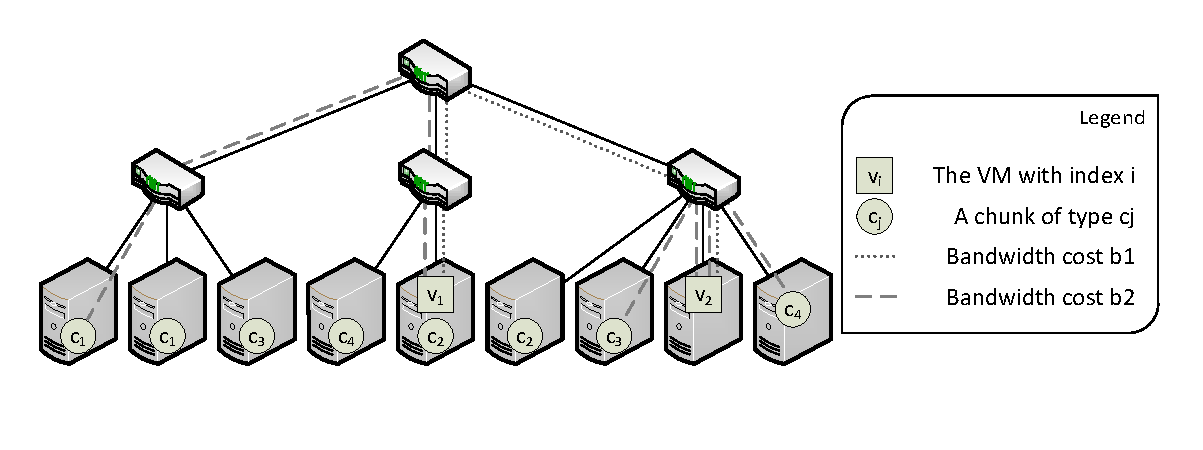
\includegraphics[width=0.99\columnwidth]{figs/overview-fig.pdf}
\caption{Overview: a 9-server (fat-tree) datacenter storing 4 different chunk
types $\{c_1,\ldots,c_4\}$. The chunk replicas need to be selected and assigned to the two
 virtual machines $v_1$ and $v_2$. In addition, the virtual machines are inter-connected among
 each other. The objective of the embedding problem is to minimize the overall bandwidth allocation.}
\label{fig:overview}
\end{figure}


%\textbf{Fundamental Parts.}

\subsection{Fundamental Parts}

Our model consists of three fundamental parts: (1) the substrate network (the servers
and the connecting physical network),
(2) the to be processed input (the data), and
(3) the virtual network (the virtual machines and the logical network connecting the machines to each other
as well as to the data).

\emph{The Substrate Network.} The substrate network (also known as the \emph{host graph}) represents the physical resources:
a set $S$ of $n_S=|S|$ servers interconnected by a network consisting of a set $R$ of servers (or switches)
and a set $E$ of (symmetric) links. Concretely, we assume that the inter-connecting network forms an (arbitrary) tree,
and that the servers are located at the tree leaves.
Each server $s\in S$ can host a certain number
of virtual machines (available server capacity $\capacity(s)$), and each link $e\in E$ has a certain bandwidth
capacity $\capacity(e)$.

\emph{The Input Data.} The to be processed data constitutes the input to the batch-processing application.
The data is stored in a distributed manner; this spatial distribution is given and not subject to optimization.
The input data consists of different \emph{chunk types} $\{\achunk_1, \ldots, \achunk_{\ChunkType}\}$,
where each chunk type $\achunk_i$ can have $r\geq 1$ instances (or replicas) $\{\achunk_{i}^{(1)},\ldots, \achunk_{i}^{(r)}\}$,
 stored at different servers.
Concretely, for each of the $r\cdot k$ replicas $\achunk_{i}^{(j)}$, we will denote by $\pi(\achunk_{i}^{(j)})$ at
which server it is stored. It is sufficient to process one replica, and we will sometimes refer to this
replica as the \emph{active} (or selected) replica.

\emph{The Virtual Network.} The virtual network consists of a set $\VirtualNodes$ of $n_V=|\VirtualNodes|$ virtual machines or compute
 units, henceforth often simply called \emph{nodes}.
Each node $v \in \VirtualNodes$ can be placed (or, synonymously, \emph{embedded}) on a server; this placement can be subject
to optimization.
Depending on the available capacity $\capacity(s)$ of server $s$, multiple nodes maybe be hosted on $s$.
We will denote the server hosting node $v$ by $\pi(v)$.
Since these virtual machines process the input data, they need to be assigned and connected to the
chunks. Concretely, for each chunk type $\achunk_i$, one replica $\achunk_{i}^{(j)}$ must be processed by exactly one virtual machine $v$;
which replica $\achunk_{i}^{(k)}$ is chosen is subject to optimization.
We will denote by $\mu$ the assignment or ``matching'' of virtual machines to chunks.
We will keep the model general, and consider both the case where there are more chunk types
than virtual machines (requiring the assignment of multiple chunks per nodes) and the case
where there are less chunks than virtual machines. (See below for motivations for the different scenarios.)
However, in order to avoid stragglers, we require that each node needs to process the same number of chunks.
Moreover, in order to ensure a predictable performance, both the connection to the chunks
as well as the interconnection between the virtual machines may have to ensure certain
minimal bandwidth guarantees; we will refer to the first type of virtual network as the \emph{access
network}, and to the second type of virtual network as the \emph{inter-connect}. The inter-connect will
is modeled as a complete network. Concretely, we assume that an  active chunk
is connected to its node at a minimal bandwidth $\CostTrans$, and a node is connected to any other node
at minimal bandwidth $\CostCom$.

%\textbf{Optimization Objective.}

\subsection{Optimization Objective}

Our goal is to develop algorithms which minimize
the \emph{resource footprint}: the overall bandwidth allocation in the datacenter for a given embedding. (Note that
the resource allocation at the servers does not depend on the replica selection or embedding.) That is,
we aim to embed the virtual machines in a locality-aware manner, close to the input data
(the chunks), as well as close to
each other. Let $\dist(v,\achunk)$ denote the distance (in the underlying physical network $\Tree$) between a node $v$ and a
chunk $\achunk$, and let $\dist(v_1,v_2)$ denote the distance between the two nodes $v_1$ and $v_2$.
We define the footprint $\Cost(v)$ of a node $v$ as follows:
$$
\Cost(v) = \sum_{\achunk\in \mu(v)} \CostTrans \cdot \dist(v,\achunk) \underbrace{+ \sum_{v' \in \VirtualNodes\setminus\{v\}} \CostCom \cdot \dist(v,v')}_{\text{only for inter-connect}},
$$
\noindent where $\mu(v)$ is the set of chunks assigned to $v$. Our goal is to minimize the overall footprint
$\Cost=\sum_{v\in V} \Cost(v)$.

%\textbf{Problem Decomposition.}

\subsection{Problem Decomposition}

In order to provide a complete picture of the tractability and intractability of different
problem variants, we decompose our problem into its fundamental parts, as described in the following.

\emph{Replica Selection ($\RS$).} The first fundamental problem is replica selection:
if the input data is stored redundantly, the algorithm has the freedom to choose a replica
for each chunk type, and assign it to a virtual machine. Note that this
selection or ``matching problem'' is non-trivial, even if the locations of the virtual machines
are already given. In the following, we will refer to a scenario
with redundant chunks by $\RS$; in the $\RS$-only scenario, the number of chunk types
is less or equal the number of nodes. Otherwise, we will add the $+\MA$ property discussed next.

\emph{Multiple Assignment ($\MA$).}
If the number of chunk types is larger than the number of virtual machines,
each node needs to be assigned multiple chunks. We will refer to such a scenario by $\MA$.
(Note that in a scenario with only $\MA$ but without $\RS$, chunk types are not redundant.)

\emph{Flexible Placement ($\FP$).} The second fundamental degree of freedom, besides replica selection and assignment,
regards the flexibility in the placement (or synonymously: \emph{embedding}) of virtual machines to physical servers.
We will refer to this aspect by $\FP$.

\emph{Node Interconnect ($\CC$).} We will distinguish between scenarios where bandwidth needs to be reserved
both from each virtual machine to its replica as well as to the other virtual machines
(i.e., $\CostTrans>0$ and $\CostCom>0$), and
 scenarios where only the access network requires bandwidth reservation (i.e., $\CostTrans>0$ and $\CostCom=0$).
 We will refer to the former scenarios
where bandwidth needs to be reserved also for the inter-connect, by $\CC$.

\emph{Bandwidth Capacities ($\BW$).} We distinguish between an uncapacitated and a capacitated scenario where the links
of the substrate network come with bandwidth
constraints, and will refer to the bandwidth-constrained version by $\BW$; the capacity of servers
(the number of virtual machines which can be hosted concurrently) is always limited.
Note that capacity constraints introduce infeasible problem instances, where it is impossible to
allocate sufficient resources to satisfy an embedding request; in this case, we will say that the
resource footprint is \emph{infinite}.

%\textbf{Remark on Practical Motivation.}

\subsection{Remark on Practical Motivation}

Our model is motivated by batch-processing applications such as MapReduce.
Such applications use of multiple compute units or virtual machines to
process data, initially often redundantly stored in a distributed file system implemented
by multiple servers.~\cite{mapreduce}
The standard datacenter topology today are fat-trees resp.~Clos topologies,~\cite{fattree}
which motivates our focus on tree-like substrate networks where servers are located at the
tree leaves.
During execution, batch-processing applications typically cycle through different phases,
most prominently, a mapping phase and a reducing phase; between the two phases,
a shuffling operation is performed, a phase where the results from the mappers
are communicated to the reducers. Since the shuffling phase can constitute a
non-negligible part of the overall runtime~\cite{orchestra},
and since concurrent network transmissions can introduce interference and
performance unpredictability~\cite{amazonbw}, it is important
to provide explicit minimal bandwidth guarantees.~\cite{talk-about}
In particular, our inter-connect (the virtual network connecting the virtual machines)
is motivated by the popular virtual cluster abstraction.~\cite{oktopus,talk-about,proteus}
In this paper, we extend this model with a notion of data-locality.
In particular, we distinguish between the bandwidth needed between replica
and virtual machine ($\CostTrans$) and the bandwidth needed between
two virtual machines ($\CostCom$); in practice, for applications with a large
``mapping ratio'', $\CostCom<\CostTrans$. Finally, note that it is frequently assumed
that the nodes implementing the mapper functionality also implement the reducer functionality,
and vice versa; however, it can also make sense to have more mappers or more reducers for
certain applications.

%%%%%%%%%%%%%%%%%%%%%%%%%%%%%%%%%%%%%
\section{Polynomial-Time Algorithms}\label{sec:poly}

The problem of embedding virtual machines and their interconnecting network,
as well as the selection and assignment of replicas,
exhibits interesting connections to classic matching and
flow problems. In this section, we point out these connections and
exploit them to devise polynomial-time algorithms for a wide range
of problem variants. We also show that a large number of problems
can be solved optimally using dynamic programming.

\begin{figure}
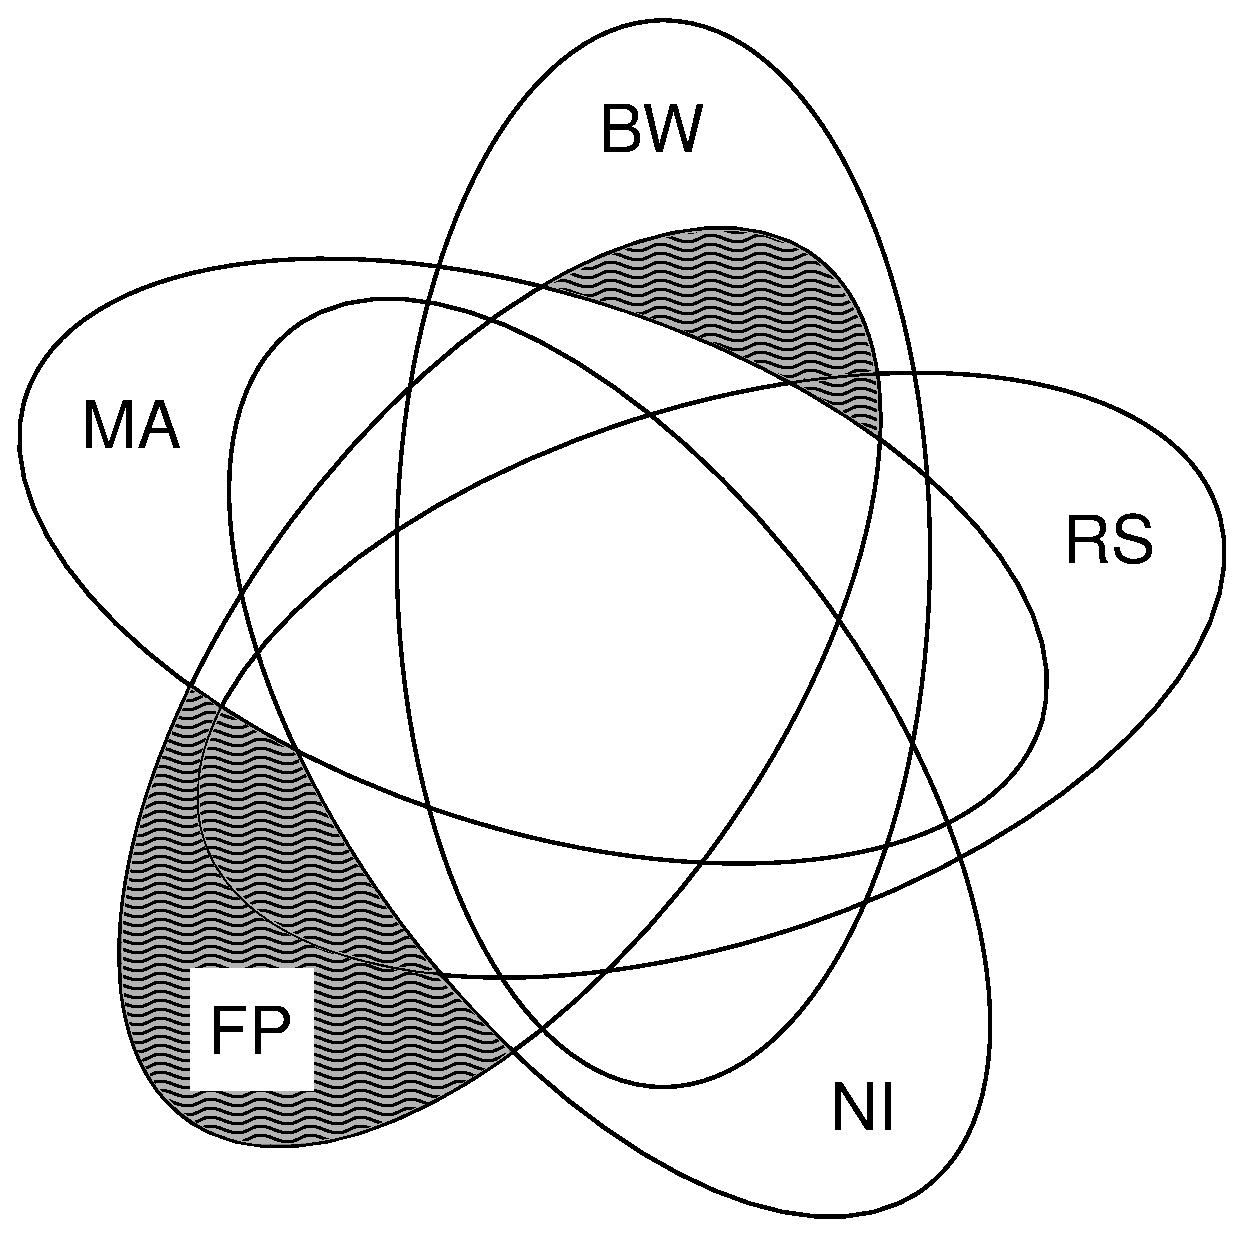
\includegraphics[width=\columnwidth]{figs/venn_trivial.pdf}
\caption{Trivially solvable property combinations}
\label{fig:venn_trivial}
\end{figure}

\carlo{A trivial strategy can solve instances with $\FP$: The strategy
collocates all VMs with chunks and hence inflicts $0$ costs, as long as $CV$ is
not a part of the problem. This strategy can even solve problem instances with
$\BW$ and $\RS$ or a combination of both. Figure~\ref{fig:venn_trivial}
shows a Venn diagram of all possible combinations of properties. The properties
which can be solved with this trivial strategy, are marked with a checked
pattern.}
%Stefan: I dont think we should say this, at least not here!
%Note that all proposed
%algorithms solve the problem optimally w.r.t. to the overall bandwidth costs
%independently of $\CostTrans$ and (if present in the properties) $\CostCom$ and
%$\Capacity$

\subsection{Flow Algorithm ($\RS+\MA+\CC+\BW$)}

\subsubsection{Introduction}

In the following section, we show how to solve
the $\RS+\MA+\CC+\BW$ problem using a flow approach.
Recall that in the $\RS+\MA+\CC+\BW$ problem,
we are given a set of redundant chunks ($\RS$) and a set of virtual machines
at fixed locations. The number of chunk types is larger than the number
of virtual machines ($\MA$), and each virtual machine needs to be connected
to its chunks as well as to other virtual machines ($\CC$), while respecting
capacity constraints ($\BW$).
Our goal is to minimize the resource footprint $\Cost$, consisting
of the bandwidth reservations in the access network and the inter-connect.

We allow an instance to have multiple virtual machines in single leaf.

We start by showing that $cv$ + $bw$ + $r$ is the same problem as $bw$ + $r$.
The placement of the $\VM s$ is given. The bandwdith function $b$ assigns
each link in the physical substrate $l_i$ a capacity $c_i$. Since the phyiscal
stubstrate is a tree there exists only one path between two nodes, and hence it
is known how much bandwidth has to be allocated on which links, in oder to
satisfy the communication between the $\VM s$. We can therefore construct a
problem with $bw$ + $r$ which has the same solutions, by defining $b'(l)$ as
$b(l) - cv_l$, where $cv_l$ denotes the amount which had to be allocated on the
link $l$ for the communication between the $\VM s$.


\subsubsection{Construction}

\carlo{Source and Sink have been swapped. check for consistency once section is 
done (remeber Figure).}

We extend the substrate network $T$ in the following way:
For each chunk type we create an artificial vertex that we connect to each leaf 
containing replica of this type by edge of capacity 1. In addition we create a 
\emph{super-source} $\Source$, and connect it to each of the artificial chunk 
type nodes. Subsequently, we create an artificial \emph{super-sink} and 
connect it to every leaf containing a VM by edge of capacity $\MaFactor$; in 
case of $x$ VMs hosted at the same leaf, we multiply available capacity of the 
edge to $x \cdot \MaFactor$. \carlo{Check model section (multiple VMs per 
Host).}

\begin{figure}
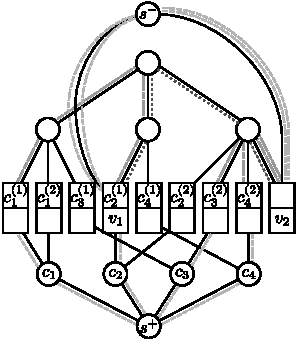
\includegraphics[width=\columnwidth]{figs/flow_ma_cv}
\caption{An example construction of a flow problem, with two VMs, four chunk 
types and two replicas of each chunk type. The maxmimal flow with minimum costs 
is indicated by the dotted lines: each line represents one unit of flow.}
\label{fig:flow_construction}
\end{figure}




We assign cost $1$ to every edge of the substrate network and $0$ to all other 
edges. We will refer to the extended graph as $G$. 
Figure~\ref{fig:flow_construction} shows an example of the extended substrate 
network: The source $\Source$ is connected, to the two leaves, which host the 
VMs. The artificial nodes are depicted below the leaves, are labled with 
their respective chunk types (e.g. $\achunk_1$), and are connected to the sink 
$\Sink$ as well as the leaves which contain replicas of their chunk type. The 
maximum flow with minimal costs is indicated by the dashed lines: each line 
represents one unit of flow. The dotted lines indicate links which have reduced 
capacity due to $\CC$.


\subsubsection{Algorithm}

Our algorithm for $\RS+\MA+\CC+\BW$ consists of two parts. First part is to compute min-cost max-flow on extended substrate network. This step is already well-known and there exists multiple algorithms for that. If we only want to know the cost of embedding, this is sufficient.

Second part is matching reconstruction. Specification of our algorithm is to produce valid matching in addition to its cost. We can do that by looking into flow that is assigned to edges at original substrate network. In order to restore a single matched pair, we start by choosing arbitrary replica $ch$ that has non-zero flow assigned to edge directly above it. Then we follow arbitrary path where there is assigned non-zero flow to the path's links. We follow the path until we reach the virtual machine $v$. We output the pair $\lbrace ch, v \rbrace$, remove replica from the tree and decrease number of available slots in $v$. We also decrease flow assigned to each edge on followed path by $1$. We continue building the matching by selecting replicas until every chunk type is processed.

\subsubsection{Algorithm correctness}


\begin{lemma}Integrality of flow
\end{lemma}
\begin{proof}
  All links have integer capacities - we just have to assume it in the model. All links have integer cost - either 0 or 1. From integer flow theorem we know that there exist integer flow and there are multiple algorithms that return such flow. One of the examples is successive shortest paths algorithm.
\end{proof}


\begin{lemma}When applied to optimal flow, path following never runs into cycles (which means that it terminates).
\end{lemma}
\begin{proof}
There are no cycles in optimal flow because $T$ is a tree and every cycle would have to go back through the same edges both ways, which would contradict optimality of the flow. This remains true in residual flow graph, because no cycles can be introduces by removing paths.
\end{proof}

\begin{lemma}
  When applied to optimal flow, path following always ends in virtual machine. Also, this virtual machine has at least one empty slot.
\end{lemma}
\begin{proof}
  Let's consider two cases:
  \begin{enumerate}
    \item path does reach the leaf, but it is empty, contains only chunk replica or contains virtual machine that does not have any slots left
    \item path does not reach the leaf
  \end{enumerate}
 Follows directly from flow optimality on extended substrate network.
 
  (1) We can transfer the same amount of flow with smaller cost by removing flow from uplink of leaf that we ended into. If we ended in leaf without the virtual machine, there is no connection from the leaf to sink; if we ended in leaf which is already full, we do not benefit from this flow as well, as no more flow can be transported by artificial edge from virtual machine to sink (as it can only transfer $vms \cdot ma$). Please note that flow is directed, therefore we cannot follow the path from replica $c_1$ to other replica $c_2$, because outgoing flow from $c_2$ (if selected) is directed upwards.

  (2) We can construct cheaper cost solution by reducing the flow on this path by $1$. We can do that without losing total flow from source to sink, because followed path didn't ended in sink.

 \maciek{This lemma can be proved by flow conservation argument together with no cycle argument. It might be better approach, as I have some doubts with (2).}
\end{proof}

\begin{corollary}Path following on optimal flow produces perfect matching of selected chunk replicas and virtual machine slots
\end{corollary}

\begin{comment}
Observation. Flow needs to be optimal for this strategy to work, otherwise we can construct such an example that reconstruction fails (because it needs to go back an edge which is disallowed) by following some path. Let's construct binary tree with vertices a,b,c,d. Chunks are in a and d, vms are in b and c. Let's say that we have found suboptimal flow of a->c and d->b. Let's attempt reconstruction. Chunk at a finds VM at b (the closest one). Chunk at d happens to go towards root (it has flow this direction). Then it is forced to go to left child of the root (the last link with flow, and it cannot go back). Then it has no path left, as it cannot go back and path to b is already taken by a.
\end{comment}



\subsubsection{Runtime and memory consumption}

\maciek{This section is under construction, no validation was performed!}

\textbf{A Note on Runtime.} There exist several polynomial-time algorithms to compute
the integral minimum cost maximum flow problem on networks with integer capacities.
One example is the \emph{Successive Shortest Path} algorithm,
whose time complexity is $\mathcal{O}(n \cdot W((n+m)\log n)
)$ time \cite{successive_shortest_path_complexity}, where $n$ is the number of
nodes in the extended graph (consisting of substrate nodes and chunks),
$m$ is the number of edges in the substrate graph ($|\SubstrateEdges| + \Vms + \RedundancyFactor
\cdot \ChunkTypes$) and $W$ is the highest capacity in the substrate
($\max(\Capacity(\SubstrateEdge))~\SubstrateEdge\in\SubstrateEdges$).

\begin{figure}
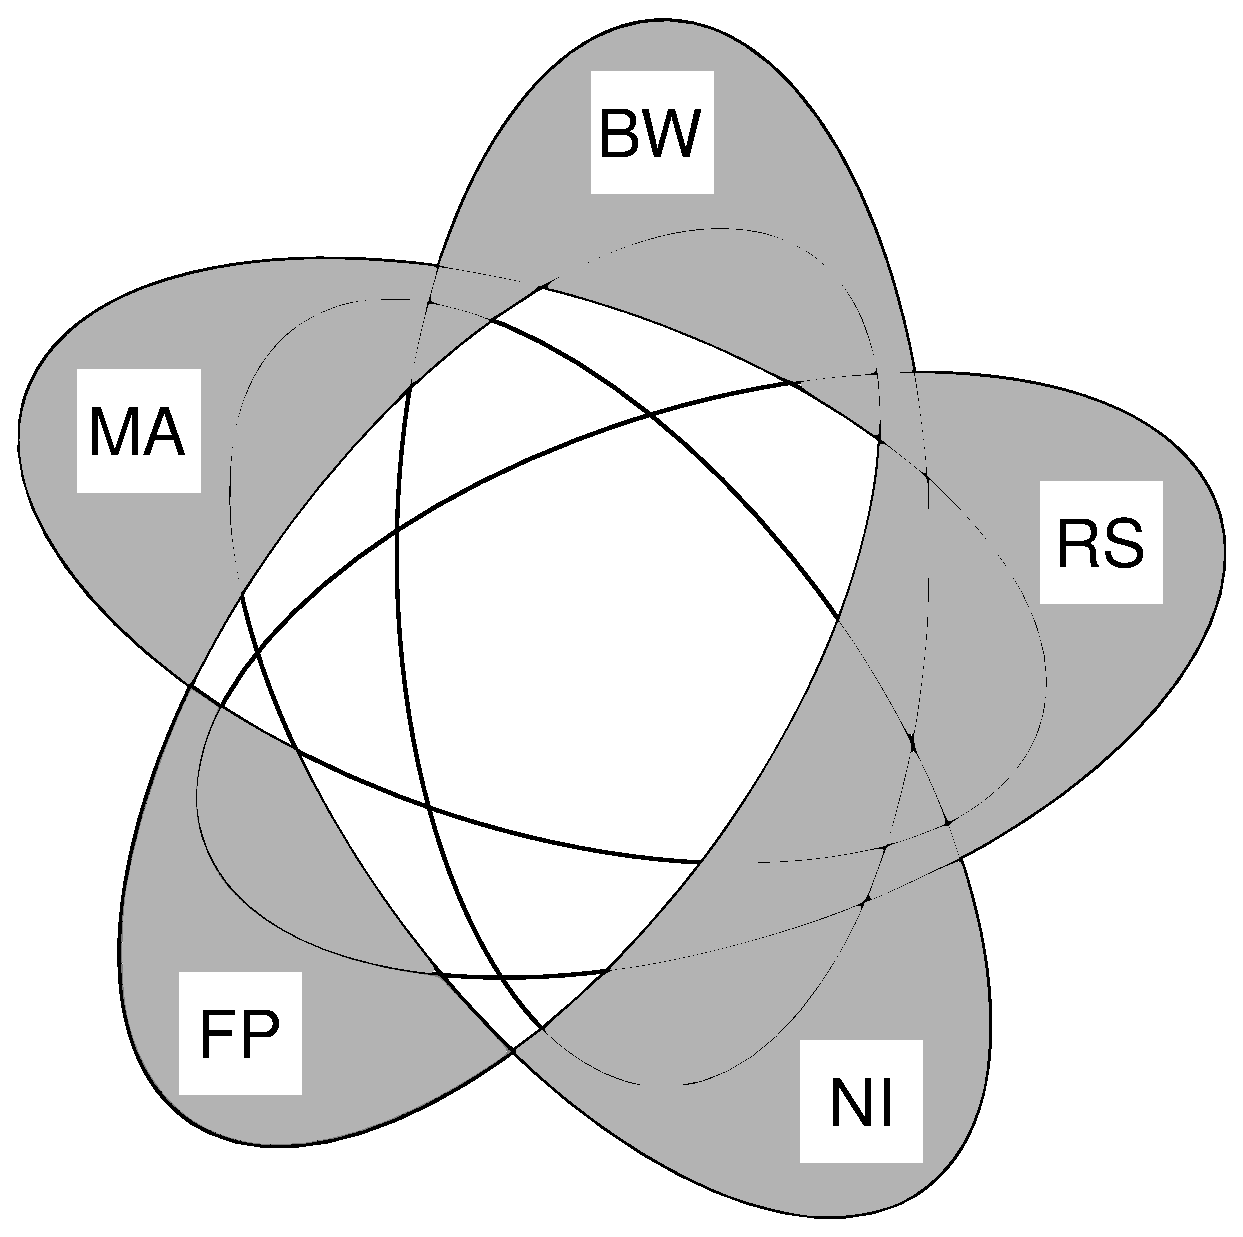
\includegraphics[width=\columnwidth]{figs/venn_flow.pdf}
\caption{Property combinations which can be solved by our flow-based algorithm.}
\label{fig:venn_flow}
\end{figure}

\carlo{Figure~\ref{fig:venn_flow} shows illustrates which problem
combiantions can be solved by the presented flow-based approach.}

\begin{comment}
\paragraph{FLOW Construction}

This section presents a flow based solution for the variant of the model which
has bandwidth limitations, communicatin between the $\VM s$ and redundant
$\achunk s$.

We start by showing that $cv$ + $bw$ + $r$ is the same problem as $bw$ + $r$.
The placement of the $\VM s$ is given. The bandwdith function $b$ assigns
each link in the physical substrate $l_i$ a capacity $c_i$. Since the phyiscal
stubstrate is a tree there exists only one path between two nodes, and hence it
is known how much bandwidth has to be allocated on which links, in oder to
satisfy the communication between the $\VM s$. We can therefore construct a
problem with $bw$ + $r$ which has the same solutions, by defining $b'(l)$ as
$b(l) - cv_l$, where $cv_l$ denotes the amount which had to be allocated on the
link $l$ for the communication between the $\VM s$.

To construct the flow graph, we start from the physical
substrate. Each edge has a associated costs of $1$ and bandwidth according the
available bandwidth due to the distribution provided by the $b$ function of the
$bw$ property of the model. In addition we create and a node for each
$\ChunkType$. Each of these nodes is connected to every node in the physical
topology, which has a $\achunk$ of the corresponding type. The capacity of these
edges is $1$ and the costs are $0$. In addition we create the source, and
connect it to all nodes, which represent $\ChunkType s$. The capacity of the
edges from the sink is $1$ and it's costs are $0$.
On this flow graph, we now solve the (integer) Max-Flow-Min-Cost Problem.

If the resulting maximal flow $\hat f$ has a value $|\hat f|< |C| = |V_V|$, the
$\Problem$ is infeasible - otherwise we can construct a solution from $\hat f$.
To construct the solution we choose an arbitrary path $p = \{e_1,\dots,
e_n\}$ \carlo{TODO check n}, such that $f(e_i) > 1 ~ \forall i \in
\{1,\dots,n\}$.
\end{comment}

\subsection{Matching Algorithms ($\RS+\MA+\CC+\BW$)}

Several problems related to replica selection,
are essentially matching problems. As we will see,
matching algorithms are often very fast, compared
to other approaches such as flow computations.

In the following, we show how to solve
the $\RS+\MA+\CC+\BW$ problem using a matching approach.
Recall that in the $\RS+\MA+\CC+\BW$ problem,
we are given a set of redundant chunks ($\RS$) and a set of virtual machines
at fixed locations. The number of chunk types is larger than the number
of virtual machines ($\MA$), and each virtual machine needs to be connected
to its chunks as well as to other virtual machines ($\CC$), while respecting
capacity constraints ($\BW$).
Our goal is to minimize the resource footprint $\Cost$, consisting
of the bandwidth reservations in the access network and the inter-connect.

We will first only discuss the simpler uncapacitated variant $\RS+\MA+\CC$, and postpone
the discussion of the capacitated extension $\RS+\MA+\CC+\BW$ to the end of the section.
Moreover, we observe that in the absence of node placement flexibilities (no $\FP$),
due to the tree structure of the substrate topology $\Tree$, the bandwidth required
for the inter-connect network can be allocated upfront, and does not depend on the replica
selection and assignment. Thus, the $\RS+\MA+\CC$ problem boils down to $\RS+\MA$.

In order to solve $\RS+\MA$, we construct a bipartite graph between the set
$\VirtualNodes$ of virtual machines and
the set of chunks.
Concretely, we clone each node $\MaFactor$ times,
as each node needs to process
$\MaFactor$ replica types, and we collect all copies of a given chunk type in a
single %$\ChunkType$
``super-node''. We connect each node to all chunk types using the
\emph{lowest hop count} to one of the copies as the cost metric (the link weight).

On the resulting graph, we can compute a Minimum Weight
Perfect Bipartite
Matching:
the matching denotes the assignment of chunks to nodes.

\begin{figure}
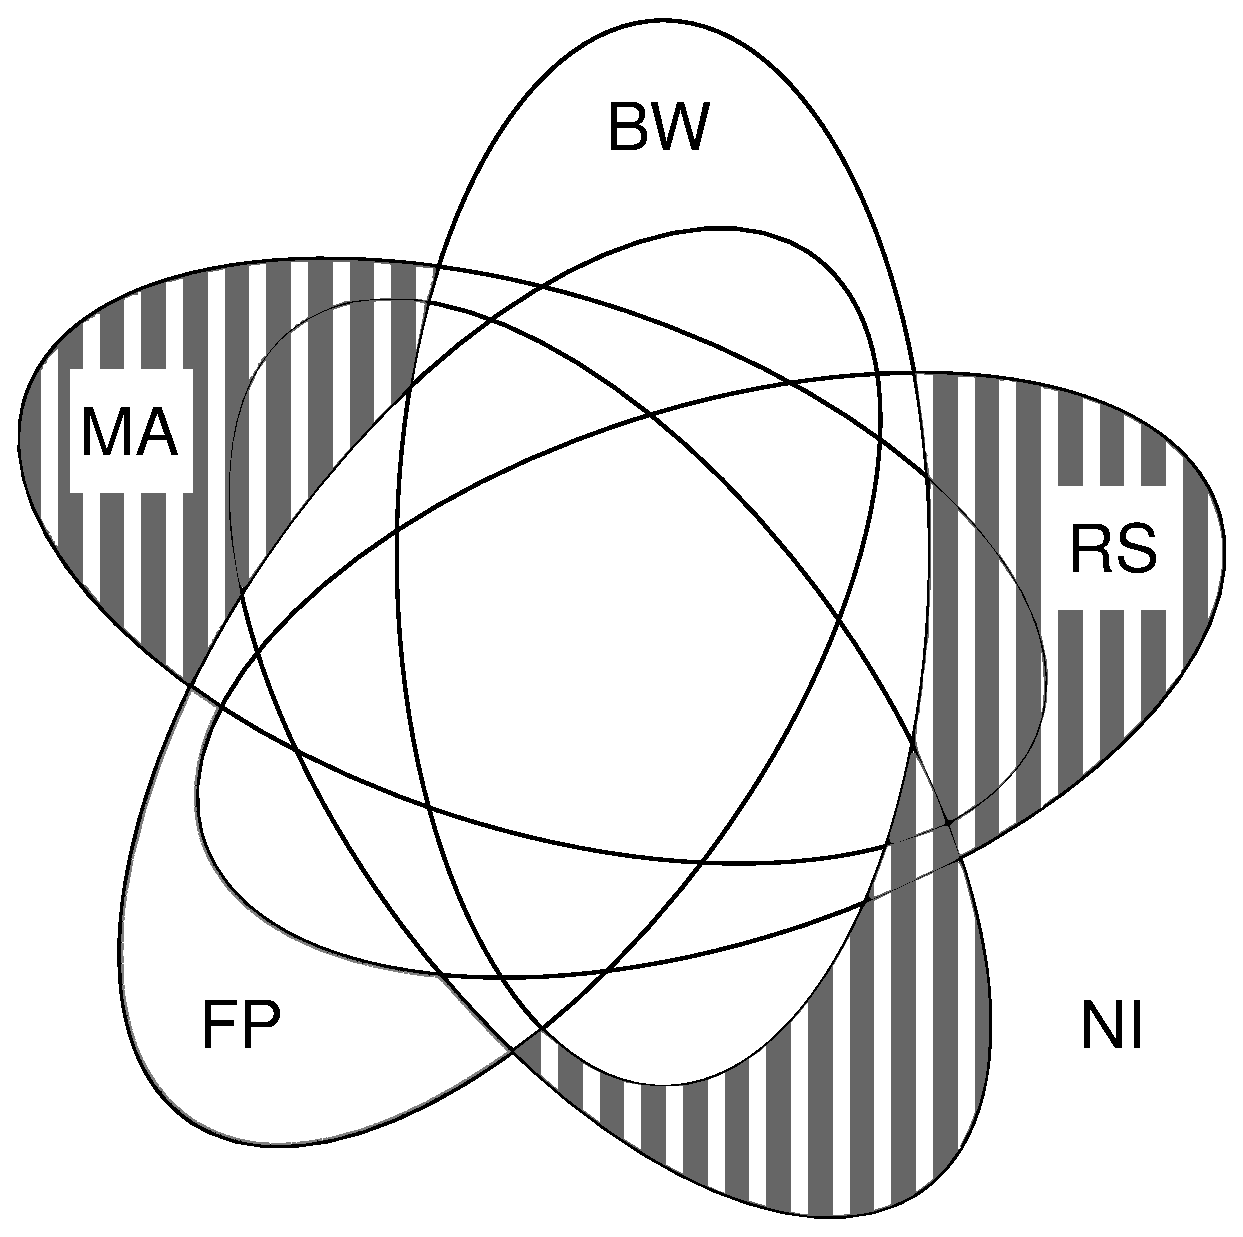
\includegraphics[width=\columnwidth]{figs/venn_matching.pdf}
\caption{Property combinations which can be transformed into matching problems.}
\label{fig:venn_matching}
\end{figure}

Figure~\ref{fig:venn_matching} provides an overview of 
which problem combinations can be solved by the presented matching approach.


\textbf{Example.} Let us give a small example.
Figure~\ref{fig:matching_basic} shows an example for the problem instance introduced in
Figure~\ref{fig:basic_problem}: $\NodeMapping(\VirtualNode_1)$ is four hops
away from all chunks; in the matching problem, this is
reflected in the corresponding edge
weights. Similarly, $\NodeMapping(\VirtualNode_2)$ is
two hops away from $\achunk_2$, and four hops away from $\achunk_1$. Hence the
weight of the edge $(\NodeMapping(\VirtualNode_2),\achunk_2)$ is $2$, while the
weight on the edge to $\achunk_1$ is $4$. The solution to the minimum weight
perfect bipartite matching contains the edges $(\NodeMapping(\VirtualNode_1),
\achunk_1)$ and $(\NodeMapping(\VirtualNode_2),
\achunk_2)$, which is exactly the chunk to node assignment $\VmChunkAssignment$
which we identified as an optimal solution in Section~\carlo{TODO}.
Figure~\ref{fig:matching} illustrates this for the scenario of
Figure~\ref{fig:model_combined}: The two nodes are
cloned into $\MaFactor = 2$ nodes each, resulting in a total of four nodes in
the matching problem. The $\RedundancyFactor = 2$ chunks of each chunk type are
aggregated $\achunk_j$ into a single chunk type node in the matching problem;
this gives a total of $4$ chunk type nodes in the matching graph. The weight
on the edges between all clones of a specific node and a chunk type are set to
the minimum distance. This can for instance be observed at the edges connecting
the two clones of $\VirtualNode_1$ to $\achunk_2$: both weights are 0.

\textbf{Runtime: Matchings are fast!}
Let us now study the runtime of the matching approach.
While matching problems can be solved in polynomial time~\cite{schrijver_combinatorial_optimization} using
general algorithms, in the following, we show that for our problem
a simple and fast greedy strategy is sufficient. 
Accordingly, we can use greedy bottom-up construction of matching. 
Its runtime is linear with respect to number of tree vertices. It is more efficient that more general methods of 
finding perfect matching in general bipartite graphs.


\begin{lemma}
A local and greedy perfect matching of chunks to nodes is optimal. 
\end{lemma}
\begin{proof}
Proof by contradiction. Let us assume that there exists matching of cost lower 
than cost of $G$. Let's take cheapest such matching and call it $H$.

Let's find smallest subtree $S$ where partial matching of $G$ has different cost than partial matching of $H$. It means that in both left and right subtree we did local matching (do we need this sentence?). It means that non-local decision was made in this subtree (perhaps hoping for savings higher?). Then there exist two such two such matched pairs in $H$ that shares an edge (one pair is transporting chunk up, the second one is transporting chunk down). Then we can create matching $H'$ that uncrosses those edges (does the local matching on them) and is cheaper than $H$. Contradiction.

\maciek{It means basically that in every subtree we can only have more costly solution. Perhaps there exist cleaner way of proving that.}
\end{proof}



\begin{figure}
\begin{minipage}[b]{0.49\linewidth}
\centering
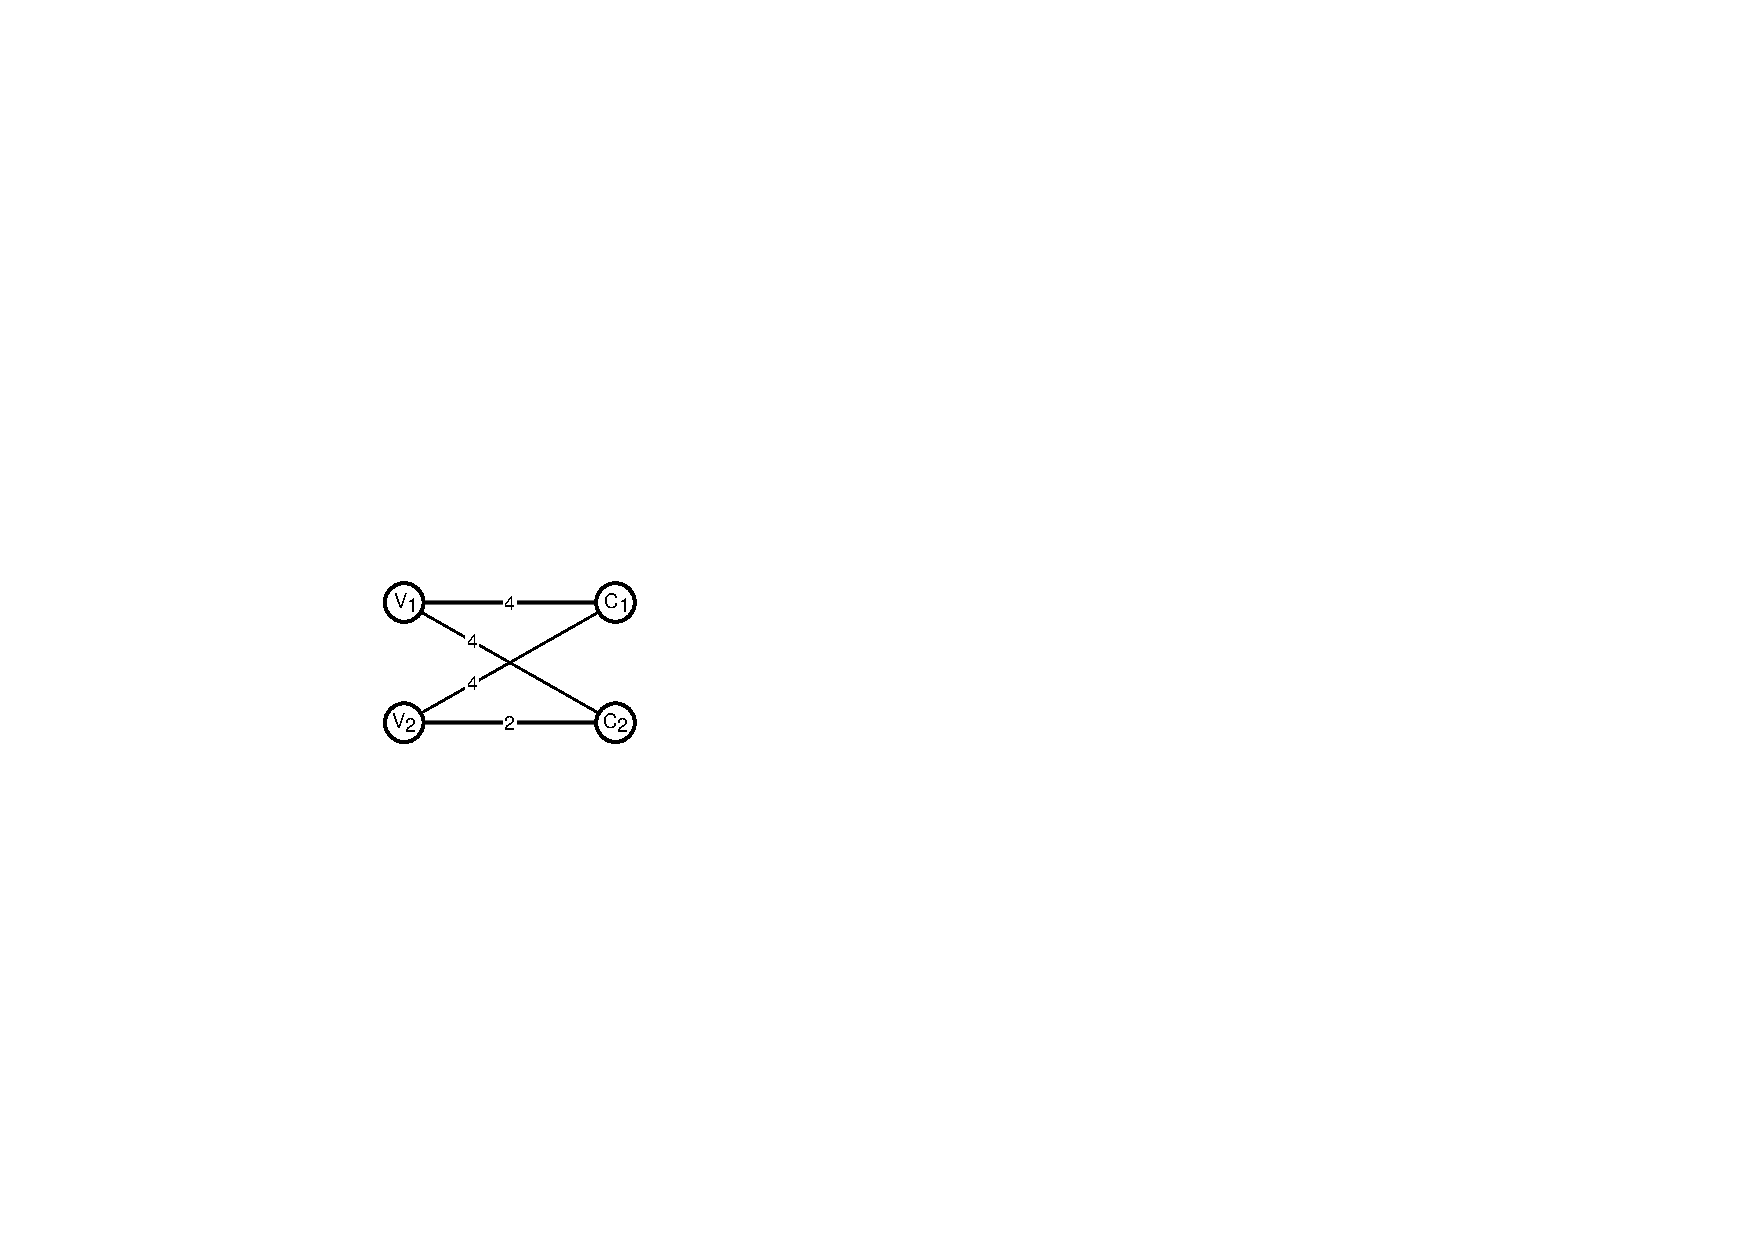
\includegraphics[width =\columnwidth]{figs/matching_basic}
\caption{The matching problem generated from the basic scenario in
Figure~\ref{fig:basic_problem}}
\label{fig:matching_basic}
\end{minipage}
\quad
\begin{minipage}[b]{0.49\linewidth}
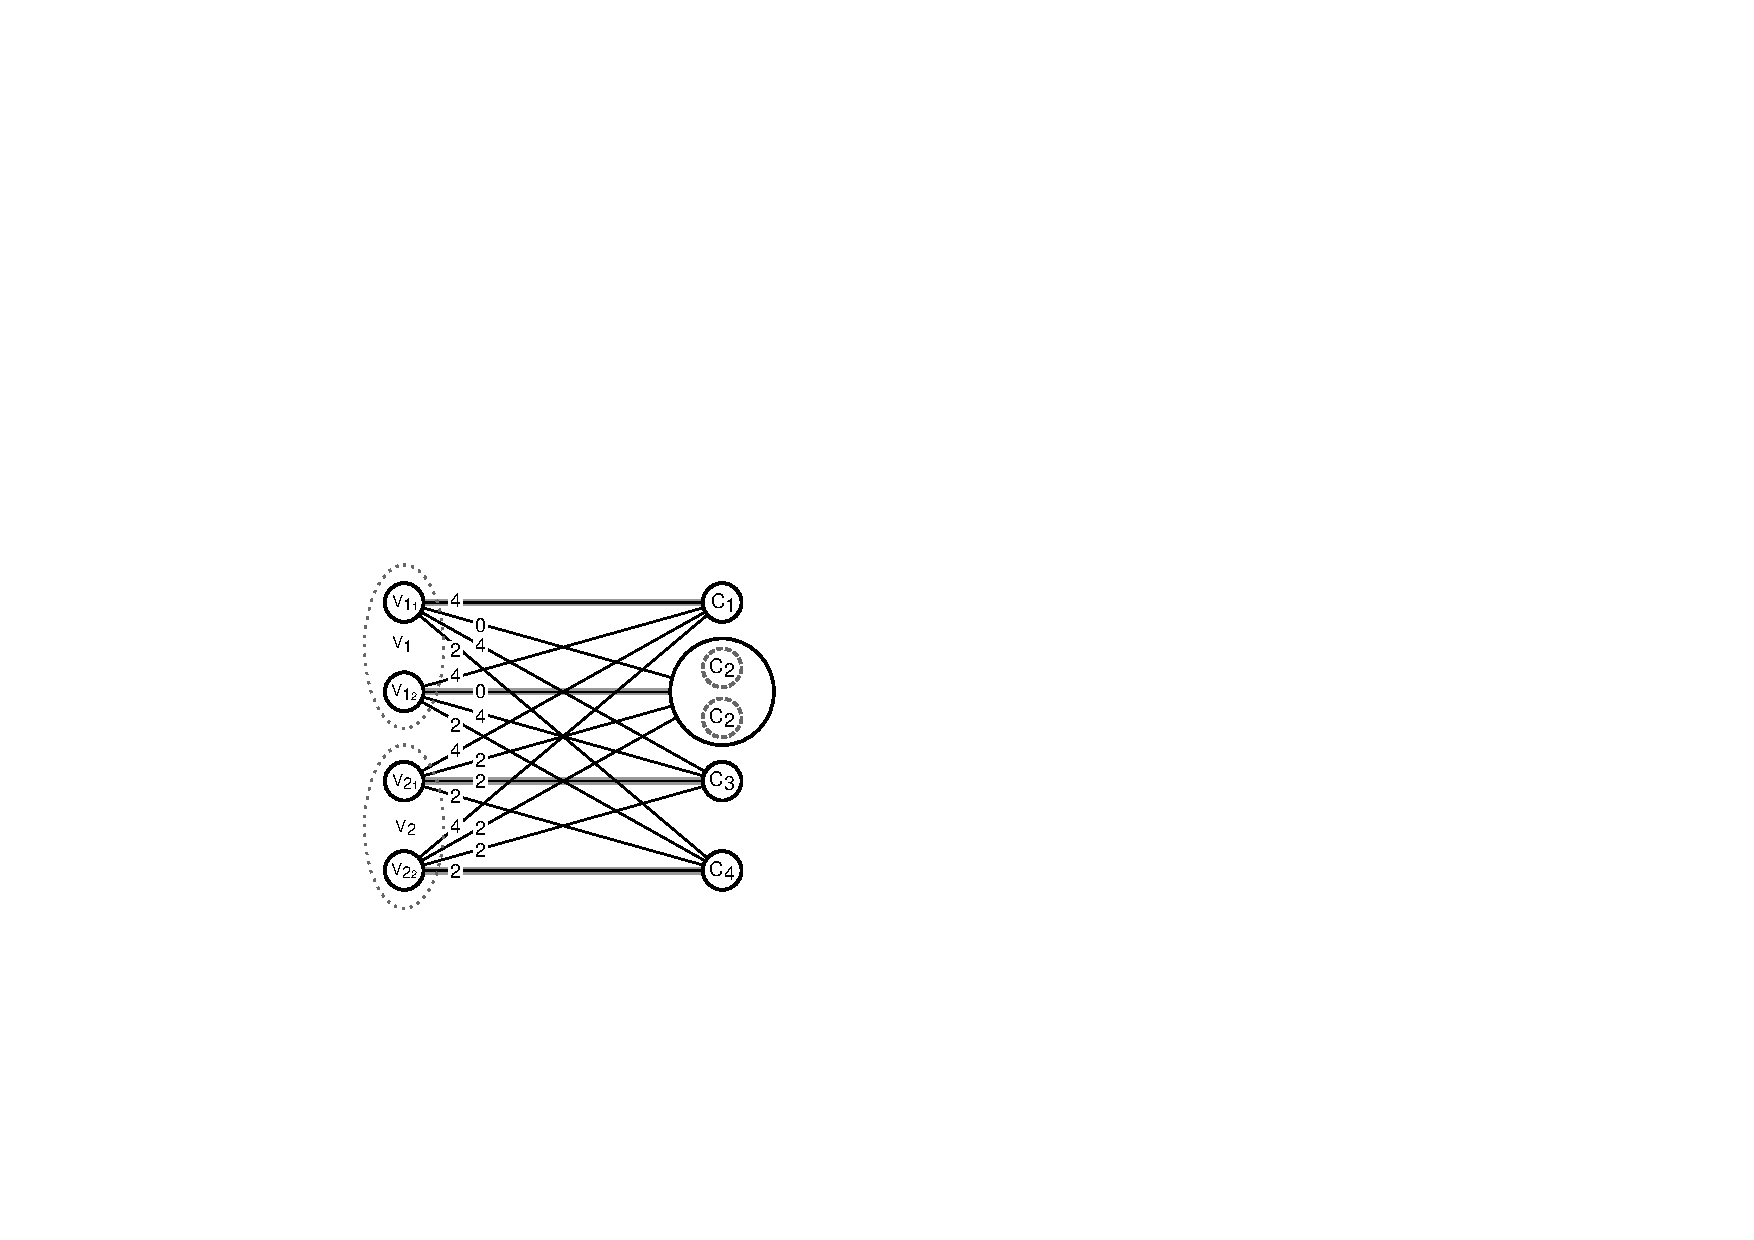
\includegraphics[width = \columnwidth]{figs/matching}
\caption{The matching problem for the instance from
Figure~\ref{fig:model_combined} without $cv$. The solution is indicated by
shadowed lines.}
\label{fig:matching}
\end{minipage}
\end{figure}

\textbf{Adding $\BW$.} Let us know show why the matching approach can also be used to solve $\RS+\MA+\CC+\BW$.

\begin{lemma}
(uplink lemma)
For every tree T (with chunks) and number of VMs $x$ the bandwidth of uplink is the same among all possible feasible solutions)

\maciek{unless we allow something as stupid as routing communication and transport through loops}
\end{lemma}


\begin{corollary}
In the abscene of $\RS$ and $\FP$, all bandwdith optimal assignments
$\VmChunkAssignment$ have identical bandwdith costs on all links in the host
graph.
\end{corollary}

This is a direct consequence of Lemma~\carlo{TODO: REF uplink lemma}, as the
amount of chunks and VMs in all subtrees is static, and all links are uplinks
of subtrees (which possibly consist of only one node).

\begin{lemma}
Given a minimal cost solution assignment $\VmChunkAssignment$ to a problem
instance with $\MA$, any bandwdith function $\capacity$, which assigns less
bandwidth to any link in the host graph then $\Cost(\VmChunkAssignment,
\SubstrateEdge)$, renders the problem infeasible.
\end{lemma}

\begin{proof}
 By contradiction. Assume the problem is still feasible, although
$\VmChunkAssignment$ exceeds the capacity on at least one link. Then there has
to be a minimal cost assignment $\VmChunkAssignment'$, with
$\Cost(\VmChunkAssignment') > \Cost(\VmChunkAssignment)$, which does not
violate the capacity on each individual link. We can now choose an arbitrary
link, which has a higher costs in $\VmChunkAssignment'$ than in
$\VmChunkAssignment$.
\end{proof}

\begin{lemma}
An instance of $\Problem$ is infeasible iff. algorithm returns $\infty$.
\end{lemma}
\begin{proof}
  ($\rightarrow$)

  ($\leftarrow$)
  \end{proof}

\maciek{I think that we do not need that lemma, it might be obvious. I leave it
there just in case.}
\begin{lemma}
  If algorithm returns solution $\Sol$ of cost $\neq \infty$, then in $\Sol$ no
link exceeds its capacity limit.
  \end{lemma}

\subsection{Dynamic Programming ($\FP+\CC+\MA+\BW$)}

Dynamic programming solutions are generally useful in for problems
exhibiting the \emph{optimal substructure property}, namely, if given
the optimal solutions of subproblems, an optimal solution for the
larger problem can be computed efficiently. 
In the following, we show that the $\FP+\CC+\MA+\BW$ problem
exhibits such a structure, and show how to exploit it to
compute efficient embeddings, even in scenarios where multiple chunks
need to be assigned to flexibly placeable nodes.

\textbf{Basic ideas.} For ease of presentation, we will transform the substrate network $\Tree$
into a binary tree, using binarization: 
The
strategy we use is to clone every node of degree $\Delta$, $\Delta(v) - 1$ times,
placing subsequent clones as right son of the previous one and placing
subsequent children as left son of the clone. Last child is placed as
right son of last clone.


\maciek{We will want to go through all VM placements, for each of those do greedy matching and choose the cheapest.}

\maciek{Solution for subtree - how it can look like? It is ``partial matching''. Some matched VMs and chunks, but also some chunks transported out of subtree or some VMs/slots that will have chunks transported into from outside. So we charge already those incomplete matchings.}

Let's begin designing our algorithm by writing recursive formula for
minimal cost inclined by placing virtual machines in leaves of a given
tree. Our approach is to evaluate this function using bottom-up
technique using auxilary array, which yields a dynamic programming
solution. To find actual placements of virtual machines in addition to
the cost, we traverse the array backwards, following the path of
minimas.

Keep in mind that number of virtual machines is equal to number of
chunks. However, our function $f$ will be defined by structural
induction on the tree and we will invalidate the property of having
the same number of chunks and virtual machines in a given subtree
(which is true when we look at whole tree).

Let's define $f$ in following way. First argument is a subtree (with
available informations like number of chunks in its leaves), and the
second argument is number of virtual machines that we decided to place
in the subtree (given as first parameter). To calculate optimum
placement of $x$ virtual machines in subtree $T$ ($f(T, x)$) we will
consider every possible split of number $x$ into two positive integer
values: $l$ and $r = x - l$. We will place $l$ virtual machines in
left subtree of $T$ and $r$ virtual machines in right subtree of
$T$. Having such information allow us to compute how much cost we
incline through edge $e_1$ (which connects left subtree of $T$ to root
of $T$) and edge $e_2$ (which connects right subtree of $T$ to root of
$T$). In a given recursive call we charge only those two edges, rest
of edges will be charged is subsequent calls.

Our cost function consists of two factors. First one, communication
cost between virtual machines is easy to compute. We know how many
virtual machines are in left subtree, how many are in right subtree
and how many are in whole tree outside of $T$. For each pair of
virtual machines, first of which is in left subtree and second of
which is in right subtree, we charge $b_2 \cdot (w(e_1) +
w(e_2))$. For each pair of virtual machines, first of which is in left
subtree and second of which is outside $T$, we charge $b_2 \cdot
w(e_1)$. Right subtree case is symmetrical. Second factor of our cost
function is the cost of transferring chunks to virtual machines. Let's
call number of chunks in left subtree as $c_l$ and number of chunks in
right subtree as $c_r$. To incline minimal cost we connect chunks in
given subtree to virtual machines in the same subtree. If we can no
longer do that, because $v_i < c_i (i \in \{l,r\})$, then we connect
leftover chunks to virtual machines in second subtree of $T$. If we
can no longer do that, we connect leftover chunks outside of $T$. This
strategy is optimal, because connecting any other way can be amended
(TODO: need better argument here), inclining lower cost. Connections
inside either left or right subtrees inclines cost $0$ to edges $e_1$
and $e_2$. Connections between left and right subtree incline cost
$b_1
\cdot (w(e_1) + w(e_2))$. Connections from either subtree to outside
of $T$ inclines either $b_1 \cdot w(e_1)$ or $b_2 \cdot
w(e_2)$. Finally, we can write down our formula for $f$:

\begin{multline}
f(T, x) = min_{l \in \{0, \ldots, x\}} \{ f(T_l, l) + f(T_r, x - l) \\
+ TransferCost(T_l,l,T_r,x-l) \\ + ConnectionCost(l,x-l)\}
\end{multline}

One simplifying observation is that to calculate $TransferCost$ we can
just use the absolute value of difference between number of chunks and
number of virtual machines in a given subtree, without knowing which
is bigger, because in our model if there are some virtual machines
left, we know that some chunks from outside will use the same transfer
as if we have excessive chunks in the subtree.

\subsection{Algorithm}
\newcommand{\SumIndex}{\ensuremath{n}}
\begin{algorithm}[tbhp]
\DontPrintSemicolon % Some LaTeX compilers require you to use
%%\dontprintsemicolon instead
\SetAlgoNoEnd
\KwIn{$\Opt_{\SubstrateNode_l} ,
\Opt_{\SubstrateNode_r},
\ChunkCount_{\SubstrateNode_l},\ChunkCount_{\SubstrateNode_r} $}
$\ChunkCount_\SubstrateNode = \ChunkCount_{\SubstrateNode_l} +
\ChunkCount_{\SubstrateNode_r}$\;
\For{$\SumIndex \in \{0,\dots,\Vms\}$}{
  \For{$i \in \{0,\dots,\SumIndex\}$}{ \If{$\Opt_\SubstrateNode[\SumIndex]
  > \Opt_{\SubstrateNode_l}[i] +
\Opt_{\SubstrateNode_r}[\SumIndex - i]$}{
	$\Opt_\SubstrateNode[\SumIndex] \gets \Opt_{\SubstrateNode_l}[i]
	+
\Opt_{\SubstrateNode_r}[\SumIndex - i]$\;
    } }

 $bw \gets (\Vms -
\SumIndex) \cdot \SumIndex \cdot \CostCom +   |i -
\ChunkCount_\SubstrateNode| \cdot \CostTrans$\;
  \eIf{$bw \leq \Capacity(\Uplink(v))$}{
    $\Opt_\SubstrateNode[\SumIndex] \gets \Opt_\SubstrateNode[\SumIndex]
    + bw$\; }{ $\Opt_\SubstrateNode[\SumIndex] \gets \infty$\; } }
%
\caption{$aggregate(\SubstrateNode \in \SubstrateNodes)$}
\label{algo:dynAggregation}
\end{algorithm}

List all needed functions like distance, counter of number of chunks
in subtree.

Tell how to go back through the array to reconstruct the actual
placements. Following path of minimas. Other approach is to store pointers to minimas on lower levels as those are chosen.

(Base case) We fill the entire array $Opt_l$ for the leaf $l$ with zeros. It means that we allow hosting $0, 1, \ldots, n$ VMs in this leaf. We can restrict the number of VMs that are hosted in the same leaf by some constant $x$ (that can be independent for every leaf) by setting $Opt_l[x+1] = Opt_l[x+2] = \ldots = Opt_l[n] = \infty$.

\subsection{Algorithm correctness}

\subsubsection{Bandwidth correctness.}

\begin{lemma}
Let's say that we calculated solution for our instance of VC with
ignoring the bandwidth. Then we analyzed every link and it turned out
that some of them exceed their capacity. Then the instance is
infeasible and we cannot fix that by choosing any other matching (even
suboptimal one).
\end{lemma}

It might happen that this lemma does not hold, beware!

\maciek{Below there is emergency lemma in case that above lemma does not hold. In case above lemma is true it implies that below lemma is true.}
\begin{lemma}
An instance of $\Problem$ is infeasible iff. algorithm returns
$\infty$.
\end{lemma}
\begin{proof}
  ($\rightarrow$)

  ($\leftarrow$) \end{proof}

\maciek{I think that we do not need that lemma, it might be obvious. I leave it there just in case.}
\begin{lemma}
  If algorithm returns solution $\Sol$ of cost $\neq \infty$, then in
  $\Sol$ no link exceeds its capacity limit.  \end{lemma}

\subsubsection{Substructure optimality without bandwidth.}

Definition of partial matching (matching + transporting imbalanced
chunks out of tree and transporting chunk into imbalanced VMs from
outside the tree). Definition of partial matching optimality
(parametrized by number of VMs, subtree and chunks; best among all
possible that match the same chunks and transports the imbalance).
\begin{lemma}

Let's consider an arbitrary tree $T$ with chunks $c_i$ and number of
VMs $v$. Than $f(T, v)$ is cost of optimal partial matching.

\end{lemma}

\begin{proof}
Proof by structural induction. First, we take definition of $f$, which
contains values of $f$ for left and right subtree for different number
of VMs (but which sum to $v$). We can assume by induction that those
are optimal. Then we calculate the cost of communication and matching
between left and right subtree (also in $f$'s definition. Then we
choose the minimum cost one. We argue that this one is optimal partial
matching, and we use optimality of greedy matching for that.

Also, we use the uplink lemma to show that choosing optimal partial
matching in left and right subtree does not generate excessive
bandwidth on both uplink edges (we might have doubted that because
optimal partial matchings were restricted to their subtrees and we
might thought that there is some other more costly matching that has
less bandwidth on uplink - to save there).

Also, we use optimality of greedy matching that is in matching
chapter.
\end{proof}

\subsubsection{Substructure optimality with bandwidth.}
\begin{lemma}
Function $f$ modified to take bandwidth into account returns cost of feasible optimal partial matching (or no feasible solution exists).
\end{lemma}

\begin{proof}

For a given positions of VMs if optimal matching is infeasible, no other (even suboptimal) matching is feasible. Our algorithm checks every possible placement of VMs, so if there would be any feasible placement, our algorithm would have found feasible matching for that (the optimal one).

\end{proof}
\subsection{Running time and memory consumption analysis}

We spend certain amount of time in every of $2|T|$ vertices of binary
tree (factor 2 is inclined there because of binary
transformation). This time can be bound by iterating over splits of
$n$ into two integers, times some constant and we do it for every
possible number of VMs from $0$ to $n$. Therefore, resulting running
time is $O(Nn^2)$.

\begin{figure}
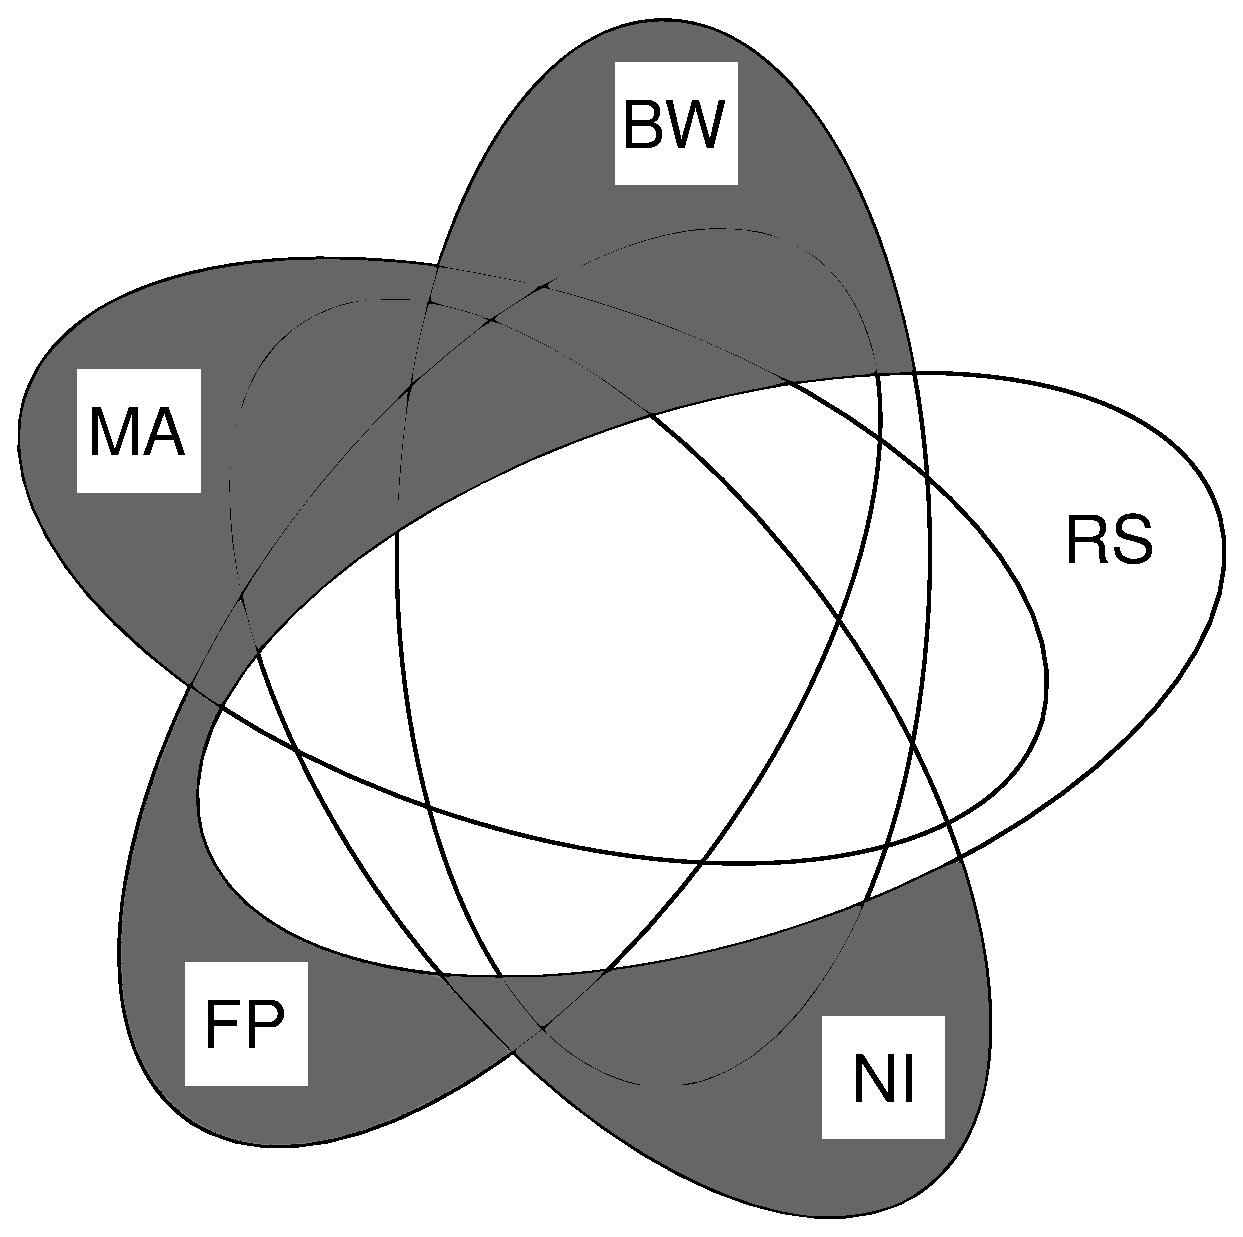
\includegraphics[width=\columnwidth]{figs/venn_dp.pdf}
\caption{Property combinations which can be solved by our dynamic prorgramming
appraoch.}
\label{fig:venn_dp}
\end{figure}

\carlo{Figure~\ref{fig:venn_dp} shows illustrates which problem
combiantions can be solved by the presented dynamic programming
approach.}

%%%%%%%%%%%%%%%%%%%%%%%%%%%%%%%%%%%%%
\section{NP-Hardness Results}\label{sec:np}

\begin{figure}
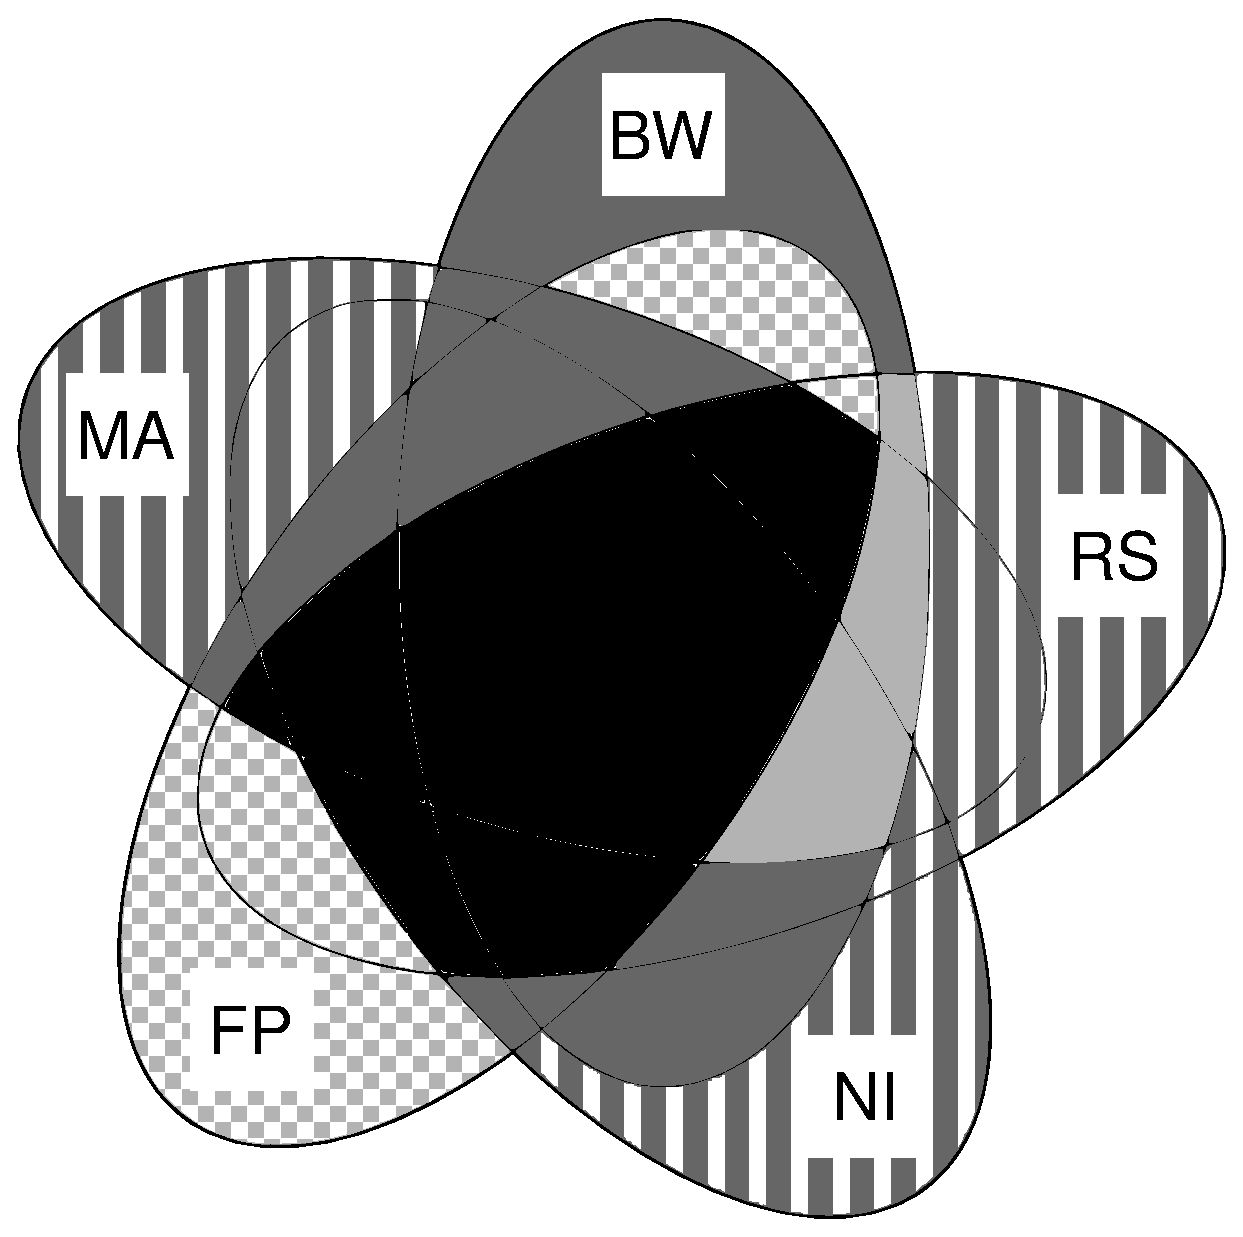
\includegraphics[width=\columnwidth]{figs/venn_full.pdf}
\caption{Trivially solvable property combinations}
\label{fig:venn_full}
\end{figure}

\carlo{TODO: Move embedd in surrounding text / move. Figure~\ref{fig:venn_full}
gives an overview of the problems, which have been solved in polynomial time in
Section~\ref{sec:poly}. This section will present proofs to show that all
remaining property combinations (marked in black) are np-hard.}

We have seen that even problems with multiple dimensions of
flexibility can be solved in polynomial time. We presented dynamic programming-based solution for
jointly optimization of flexible node placement, assigning multiple
chunks to the same VM, communication among VMs, even under capacity
constraints ($\FP+\MA+\CC+\BW$). We were able to produce solution for optimizing replica selection,
multiple assignment, VM communication, under capacity constraints in
scenario where VMs are already spawned in certain nodes ($\RS+\MA+\CC+\BW$).



This section now points out fundamental
limitations in terms of computational tractability. In particular, we
will show that problems become NP-hard if multiple replicas have to be
assigned to a node ($\FP+\RS+\MA$ is proved NP-hard in
Section~\ref{ssec:fprsma}) or if inter-connects have to be established
($\FP+\RS+\CC$ is proved NP-hard in Section~\ref{ssec:fprscc}); both
results hold even in uncapacitated networks, and even in trees
consisting of two levels only (e.g., in a
datacenter \emph{pod}). Hardness of those problem variants will result
in hardness of 4 other variants -- see generalization graph below.


\begin{figure}[htbp]
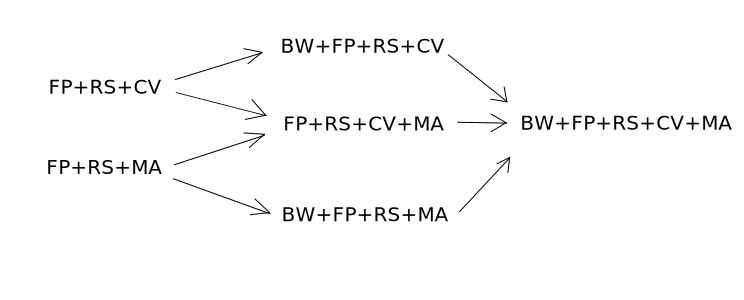
\includegraphics[width = \columnwidth]{figs/np-hierarchy}
\end{figure}



\subsection{Introduction to 3D Perfect Matching}

We start by introducing the NP-complete problem of 3D Perfect Matching
that will serve as problem we reduce from in both proofs. This problem
can be seen as a generalization of bipartite matchings to 3-uniform
hypergraphs, henceforth called $\TDM$.~\cite{3dmatch}

$\TDM$ is defined as follows. We are given three finite and disjoint
sets $X$, $Y$, and $Z$ of cardinality $k$, as well as a subset of triples $T\subset
X \times Y \times Z$.  Set $M \subseteq T$ is a 3-dimensional matching
if and only if, for any two distinct triples $(x_1, y_1, z_1) \in M$
and $(x_2, y_2, z_2) \in M$, it holds that $x_1\neq x_2$, $y_1\neq
y_2$, and $z_1\neq z_2$. Our goal is to decide if we can construct
such $M \subseteq T$ that is perfect, which means that it covers all
elements of $X \times Y \times Z$.

TODO: cite Karp on result of NP-completeness
TODO: image like this: \url{https://upload.wikimedia.org/wikipedia/commons/thumb/5/50/3-dimensional-matching.svg/240px-3-dimensional-matching.svg.png}

\subsection{Multi-Assignments are hard ($\FP+\RS+\MA$)}\label{ssec:fprsma}

Here we will present high-level ideas about encoding $\TDM$ as
 $\FP+\RS+\MA$ instance:

 \begin{itemize} \item For every element of universe $X\cup Y\cup
 Z$, we create chunk type. Processing every chunk corresponds to
 covering whole universe.

 \item We will encode each tripple as $3$ leaves that are close to
 eachother. We place chunk replicas that correspond to elements of the
 tripple.

 \item Placement of VMs will correspond to choice of tripples. No
 matter in which leaf of the gadget the VM will spawn, we will take
 that tripple to solution. VM will process the chunk that it sits on
 top of, as well as chunks in other two leaves of the same gadget.
 
\item We will set threshold cost in such way that no VM process
any chunk outside of the gadget that VM sits in.
\end{itemize}

\textbf{Construction.}
Given an instance $I$ of $\TDM$, we construct an instance $I'$ of
$\FP+\RS+\MA$ as follows:
\begin{itemize}
\item (tree construction) We create a tree consisting of root vertex, and for each tripple
we create a gadget that we attach as direct child of the root. Each
gadget consists of four vertices, one being inner node and three
leaves (see figure below).
\item (chunks and chunk replicas) For each element in $X$, $Y$ and $Z$ we create chunk type
($3 \cdot k$ in total). For each tripple we create $3$ replicas of
chunks that correspond to elements of universe and we place those
replicas in leaves of corresponding gadget
\item (other properties) We set number of VMs to spawn to $k$; we set
$\CostTrans=1$; we set number of slots in each VM to $m=3$; we set
$\Thr=2 \cdot 2 \cdot k$
\end{itemize}

FIXME: The construction is illustrated in Figure~\ref{fig:fprsma}.

\textbf{Correctness.}
We can now show the computational hardness.
\begin{theorem}
$\FP+\RS+\MA$ is NP-hard.
\end{theorem}
\begin{proof}
Let $I$ be an instance of $\TDM$ and let $I'$ be an instance of
$\FP+\RS+\MA$ constructed as described above.
We prove that $I'$ has solution of cost $\leq \Thr$ if ($\Rightarrow$) and only if
($\Leftarrow$)
$I$ has a matching of size $k$.

($\Rightarrow$) Let us take a solution to $\TDM$. We spawn VM in every
gadget that corresponds to chosen triples. We match every chunk in a
gadget to machine in this gadget (only for chosen ones). Solution has
cost exactly $\Thr$.

($\Leftarrow$) Let's take solution to $VC$ instance of cost $\leq \Thr$. We
chose triples that correspond to gadgets where were VMs. Everything
was processed, therefore every element of X,Y and Z is matched.
\end{proof}


\subsection{Inter-connects are hard ($\FP+\RS+\CC$) (reduction from 3D Perfect Matching)}\label{ssec:fprscc}


Next, we prove that the joint optimization of node placement and replica selection
is NP-hard if an inter-connect has to be established between virtual machines.
In our terminology, this is the $\FP+\RS+\CC$ problem.


\textbf{Construction.}
Given an instance of $\TDM$, we construct an instance of a
$\FP+\RS+\CC$ problem as follows. For each element
in the universe $X \cup Y \cup Z$, we construct a chunk; and for each
tripple $T_i$, we construct a gadget that contains
three replicas of chunks corresponding to the elements in the subset (those have 2 hops distance to eachother).
We connect the gadgets to the root, separating nodes from different tripples by 4 hops.

Concretely, let $I$ be an instance of $\TDM$. We will create an instance $I'$
for $\FP+\RS+\CC$ as follows:
\begin{itemize}
\item We set the access cost $\CostTrans$ to a chunk replica to a high value $W$. This will force
nodes to be collocated with the replica.
(For now, we can assume that $W=\infty$; a lower and sufficient bound will be given
in the appendix.)
\item The communication cost in the inter-connect is set to $\CostCom = 1$.
\item The number of nodes (virtual machines) is $\Vms = 3 \cdot k$. TODO: check again
\item We use a threshold $\Thr =  3 \cdot k + 3 \cdot 3 \cdot 2 \cdot (k - 1)$. TODO: check again
\end{itemize}

We construct a height-2 substrate tree
as follows. For each $T_i$ we construct a gadget
consisting of an inner node (a router) and three leaves. Every gadget
contains three chunks, corresponding to the elements of $T_i$.

FIXME: The construction is illustrated in Figure~\ref{fig:fprscc}.

\textbf{Proof of correctness.}
Intuitively, in order to minimize embedding costs,
nodes should be placed on near-by replicas. We use the following
helper lemma.
\begin{lemma}\label{lemma:helper}
In every valid solution $\Sol$ of $I'$ of cost $\leq \Thr$, each gadget
falls in one of two categories:
$k$ gadgets have exactly
$3$ nodes, and $n-k$ gadgets remain empty.
\end{lemma}
\begin{proof}
TODO: use exact cover property here to reason about feasibility

Since $W=\infty$, nodes will always be placed
directly on chunks (the access network cost is zero).
Moreover, since
$\Sol$ is valid, $3 \cdot k$ nodes are mapped
directly to the different chunk locations.
Now, consider any pair of nodes communicating over the
inter-connect; due to our construction, the communication cost
for each such pair is either
2 hops (if they belong to the same gadget) or 4 hops (if they belong
to different gadgets).
The lemma then follows from the observation that $\Thr$
is chosen such that it is never possible to distribute nodes
among more than $k$ gadgets, and that it is always strictly better to
have exactly 0 or 3 nodes per gadget, than any alternative distribution.
\end{proof}

\begin{theorem}
$\FP+\RS+\CC$ is NP-hard.
\end{theorem}
\begin{proof}
Let $I$ be an instance of $\TDM$ and let $I'$ be an instance of
$\FP+\RS+\CC$ constructed as described above.
We prove that $I'$ has solution of cost $\leq \Thr$ if ($\Rightarrow$) and only if
($\Leftarrow$)
$I$ has a solution.

($\Rightarrow$) In order to compute a solution
for $I'$ given a solution for $I$, we proceed as follows.
Given a covering set of tripples $S = \{T_1, T_2, \ldots, T_k\}$, we place three nodes in each gadget that
corresponds to every tripple of $S$. Chunks are matched to VMs that sit on top of them.

The solution has the following cost:
(1) the communication cost inside a gadget is $2 \cdot {3 \choose 2}$,
  as every pair contributes two hops;
  (2) the communication cost from each gadget to all other gadgets is $4
  \cdot 3 \cdot 3 \cdot (k - 1) / 2$, where the factor $2$ is
  for the
  communication over $4$ hops, the factor $3$
  corresponds to the number of nodes per gadget, and
  $3 \cdot (k-1)$ is the number of nodes in remote gadgets;
  as we count each pair twice, we need to divide by two in the end.
Summing up over all $k$ gadgets, we get exactly $\Thr$.

($\Leftarrow$) Given a solution for $I'$,
we can exploit Lemma~\ref{lemma:helper} to construct a solution for $I$.
We know that in any solution of cost at most $\Thr$,
$k$ gadgets contain exactly 3 nodes. These gadgets correspond to a valid
3D Perfect Matching of size $k$: every
chunk and hence element in the $X \cup Y \cup Z$, is matched.
\end{proof}




%%%%%%%%%%%%%%%%%%%%%%%%%%%%%%%%%%%%%
\section{Related Work}\label{sec:relwork}

There has recently been much interest in programming models and distributed
system architectures for the processing and analysis of big data (e.g.~\cite{nodb,mapreduce,shark}). The model studied in
this paper is motivated by MapReduce~\cite{mapreduce} like batch-processing applications, also known
from the popular open-source implementation \emph{Apache Hadoop}.
These applications
generate large amounts of network traffic~\cite{orchestra,talk-about,amazonbw},
and over the last years, several systems have been proposed which provide
a provable network performance, also in shared cloud environments, by supporting explicit
relative~\cite{faircloud,elasticswitch,seawall}
or, as in the case of our paper, \emph{absolute}~\cite{oktopus,secondnet,drl,gatekeeper,proteus} bandwidth reservations
between the virtual machines.
In particular, the notion of virtual networks which combine compute and network resources has been introduced.
For a good survey on network virtualization and in particular virtual network embeddings,
we refer the reader to~\cite{boutaba-survey} and~\cite{fischer-survey}.

The most popular virtual network abstraction for batch-processing applications today is the \emph{virtual cluster},
introduced in the Oktopus paper~\cite{oktopus}, and later studied by many others~\cite{talk-about,proteus}.
Several heuristics have been developed to compute ``good'' embeddings of virtual clusters: embeddings
with small footprints (minimal bandwidth reservation costs).\cite{oktopus,talk-about,proteus}
The virtual network embedding problem has also been studied for more general graph abstractions
(e.g., motivated by wide-area networks).~\cite{infocom2009,ammar,turner,simannealing,ucc12mip,zhu06}

From a theoretical perspective, the virtual network embedding problem can be seen as a generalization
of classic VPN graph embedding problems~\cite{Goyal2008,gupta2001provisioning},
in the sense that in virtual network embedding problems, also the embedding endpoints are flexible and subject to optimization.
In this sense, the virtual network embedding problem can also be seen as a generalization of the
classic NP-hard Minimum Linear Arrangement problem which asks for the
embedding of guest graphs on a simple \emph{line topology} (rather than tree-like topologies as
studied in this paper).~\cite{mla,mla-survey}
There exist several interesting algorithms for the Minimum Linear Arrangement problem,
e.g., providing sublogarithmic approximation ratios~\cite{mla-feige}.

However, to the best of our knowledge, we are the first to provide an algorithmic
study of the cloud application embedding problem which takes into account
data locality as well as the possibility to select replicas. As we have shown in this paper,
the resulting problems can be seen as interesting new variants of several classic optimization
problems, such as hitting set and 3-dimensional matching problems~\cite{3SC-hard} as well as cover and flow problems~\cite{korte2002combinatorial}.

%%%%%%%%%%%%%%%%%%%%%%%%%%%%%%%%%%%%%
\section{Summary and Conclusion}\label{sec:conclusion}

This paper investigated data data locality aware algorithms which exploit two fundamental
degrees of freedom in virtual cluster
embedding problems: replica selection and flexible node placement. We
decomposed the problem into its fundamental aspects,
namely $\RS$, $\MA$, $\FP$, $\CC$, and $\BW$, and studied the computational
tractability of different combinations.

In particular, we have shown that
at the heart of our model lie interesting new variants of classic
optimization problems related to matchings and flows. Interestingly, despite the
different dimensions of flexibility (in terms of replica selection, assignment and embedding),
many problem instances can actually be solved in polynomial time.
On the negative side, we have also shown that there exist computationally hard
problems even in uncapacitated networks. In particular,
we have shown that several embeddings problems are NP-hard already in two- and three-level trees
(a practically relevant result given today's datacenter topologies~\cite{fattree}),
and even if the the number of replicas is bounded by two.


Our results are summarized in
Figure~\ref{fig:summary}.
One interesting takeaway from this figure regards
the question which properties render the problem
NP-hard. For instance, we see that interestingly, $\BW$
does not influence the hardness of any problem variant,
while $\RS$ is crucial for NP-hardness.
$\MA$ only affects hardness if combined with $\RS$.
$\CC$ is trivial without $\FP$, and $\FP$ requires
more sophisticated algorithms when combined with $\CC$ or $\MA$;
in combination with $\RS$ and $\MA$ or $\CC$, $\FP$ renders the
problem NP-hard.

\begin{figure}[t]
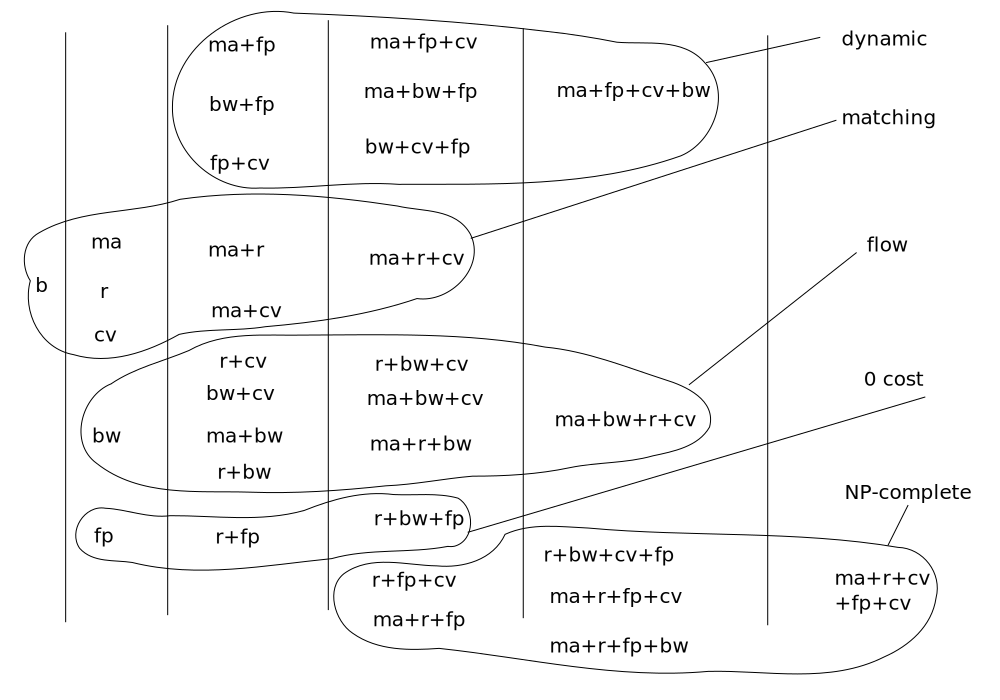
\includegraphics[width = \columnwidth]{figs/summary}
\caption{Summary of results. As this paper only presented algorithms for the most
difficult problems and, respectively, proved NP-hardness of the simplest
problems, several additional results are simple implications (indicated by arrows).}
\label{fig:summary}
\end{figure}


Our paper provides an almost complete overview of what can and cannot be
computed optimally in our setting, and may be of interest both to the algorithm
and the networking community. At the same time, we understand our model and work
as a first step, and believe that our paper opens several interesting
questions for future research, for instance, regarding randomized algorithms
or approximation algorithms.


%%%%%%%%%%%%%%%%%%%%%%%%%%%%%%%%%%%%%
%\bibliographystyle{alpha}
\bibliographystyle{abbrv}
\bibliography{references}

%%%%%%%%%%%%%%%%%%%%%%%%%%%%%%%%%%%%%
\begin{appendix}


\section{Bandwidth Lemma}

The following lemma is useful in our NP-hardness proofs.

\begin{lemma}[Bandwidth Lemma]\label{lem:bandwidth-lemma}
  Let $\clauses$ and $\variables > 4$ be two arbitrary positive integers. Let $a_1, a_2, \ldots,
  a_{\variables}$ be a sequence of $\variables$ integers which adds up to $\clauses \cdot \variables$. Also, for
  each $i$ we have $a_i \leq 2 \cdot \clauses$. Then it holds that if
  $$ \forall_i:~~ a_i \cdot (\clauses \cdot \variables - a_i) \leq \clauses \cdot (\clauses \cdot \variables -
  \clauses), $$
\noindent  then for each $i$: $a_i = \clauses$.
\end{lemma}
\begin{proof}
For the sake of contradiction, let us assume that there exists an index $k$ such that
$a_k \neq \clauses$. Then we can distinguish between two cases:
either $a_k<\clauses$ or
$a_k>\clauses$.

\textbf{Case $a_k<\clauses$:} If there exists a $k$ with $a_k<\clauses$,
due to the fact that the sequence adds up to $\clauses \cdot \variables$,
there must also exist a $k'$ such that $a_{k'}<\clauses$ (by a simple
pigeon hole principle). Thus, this case can
also be reduced to the second case (\textbf{Case $a_k>\clauses$}) proved
next.

\textbf{Case $a_k>\clauses$:} Since it also holds that $a_k < 2\clauses$,
$a_k$ must be of the form $\clauses + x$ for $x \in [1, \ldots, \clauses]$.
Let us consider the (bandwidth) inequality:
$$ (\clauses + x) \cdot (\clauses \cdot \variables - \clauses - x) \leq \clauses \cdot (\clauses \cdot \variables - x) $$

This can be transformed to:

$$ 0 \leq x(x - (\clauses \cdot (\variables - 2))) $$

The equation holds for $x \leq 0$ or $x \geq \clauses \cdot (\variables - 2)$,
and no
positive $x \leq \clauses$ can satisfy this inequality for $\variables > 4$. Contradiction.
\end{proof}

\begin{comment}
\section{Capacities are hard ($\RS+\FP+\BW$)}

We prove that $\RS+\FP+\BW$ is NP-hard by reduction from the Boolean Satisfiability Problem ($\SAT$).
Since $\SAT$ is a decision
problem, we transform $\RS+\FP+\BW$ into a decision problem too, by
introducing a cost threshold $\Thr$.

Let's first recall that the $\SAT$ problem asks whether a positive valuation exists
for a formula $\Formula$ with $\clauses$ clauses and $\variables$ variables.
In the following, we will only focus on $\SAT$ instances of at least four variables;
this problem remains NP-hard.

\textbf{Construction.}
Given any formula $\Formula$ in Conjunctive Normal Form (CNF) with at least four variables, we produce
a $\RS+\FP+\BW$ instance as follows. First, we construct a substrate tree $\Tree_{\Formula}$, consisting of
a root and separate gadgets for each variable of $\Formula$, each of which
is a child of the root.
The gadget of variable $\variab$ has a root, $\aroot(\variab)$, and two children:
$\positive(\variab)$ and $\negative(\variab)$. Child $\positive(\variab)$ has $\clauses$
many children $v_1, v_2, \ldots, v_{\clauses}$, and child $\negative(\variab)$ has
$\clauses$ many children $\neg v_1, \neg v_2, \dots, v_{\clauses}$. Every
gadget has the same structure: the same height and the same number of
leaves. By default, we will set the available bandwidth to be the
same everywhere, in every gadget; differences will be shown when we
will place chunks.

We set the number of virtual machines to $\Vms = \clauses \cdot \variables$.
Moreover, we define the inter-connect communication cost to be $1$,
and the access cost to be a sufficiently large constant $W$,
such that nodes must always be collocated with chunks.
(For a concrete value, use $W=$TODO).


We set the following bandwidth capacities in the substrate. There are three
levels of edges in the substrate network $\Tree_{\Formula}$ given by formula
$\Formula$: \emph{top}, \emph{middle} and \emph{bottom}.
We do not consider any capacities at the \emph{bottom} and \emph{middle} levels.
At a top-level edge, we set the bandwidth to $\clauses \cdot (\variables -
\clauses)$.

We set the number of chunks to be equal to the number of clauses, $\ChunkTypes =
\clauses$. To finish our construction, we place data chunks at
leaves, as follows: for the $i$-th clause we
construct as many replicas of chunk $\achunk_i$ as there are literals in the
clause. For each literal $\ell$ (of the form $\variab$ or $\neg \variab$) that satisfies clause $i$ we place
replica of chunk $\achunk_i$ in the leaf labeled $\achunk_{\ell_i}$.

The threshold $\Thr$ is given by the
communication cost among nodes in
a certain solution to our instance. This solution is constructed by embedding
nodes at all leaves of $\positive(\variab)$ and none at leaves
$\negative(\variab)$, for every gadget of variable $\variab$. Please note that $\Thr$
computed in such a way does not contain transportation cost. TODO: calculate
$\Thr$.

\textbf{Proof of correctness of construction.}
With our construction completed, we need to prove that it indeed
decides $\SAT$. We set the capacities such that in every gadget,
at most $\clauses$ nodes can be spawned, where $\clauses$
is the number of clauses of $\Formula$.
We can apply the Bandwidth Lemma (Lemma~\ref{lem:bandwidth-lemma}) as follows:
We interpret $a_i$ as the
number of nodes that are embedded in the $i$-th gadget, $\clauses$
as the number
of clauses and $\variables$ as the number of variables.
The LHS of the inequality of Lemma~\ref{lem:bandwidth-lemma}
is a formula for the communication cost of nodes inside the $i$-th
gadget to nodes outside the gadget. The RHS of the inequality is the
bandwidth constraint for the gadget. This implies that
any feasible solution must embed exactly $\clauses$ nodes in every gadget.


\begin{theorem}
The problem $\RS+\FP+\BW+\CC$ is NP-hard.
\end{theorem}
\begin{proof}
We will prove that formula $\Formula$ is satisfiable iff $\RS+\FP+\BW+\CC$ has
a solution of cost $\leq \Thr$.

($\Rightarrow$) Let us take any valuation $\Val$ that satisfies $\Formula$.
We will construct a solution to $\RS+\FP+\BW$ using $\Val$ in the following way.
For each variable $\variab$ in $\Formula$, we embed $\clauses$ many nodes
at the  leaves of the gadget of $\variab$. We need to choose $\clauses$ out of
$2 \cdot \clauses$ leaves to embed nodes. If $\Val(\variab) = 1$, we embed
nodes at the leaves
of $\positive(\variab)$, else we embed all nodes at leaves $\negative(\variab)$.
The solution constructed this way has cost exactly
$\Thr$, because the nodes are evenly split among gadgets, and nodes are not
distributed across $\positive(\variab)$ and $\negative(\variab)$ subtrees.

We calculate the chunk-node matching $\mu$ by assigning every chunk to
the node which is collocated with the first chunk replica. This solution is feasible
(every chunk type is processed),
because the given valuation satisfied $\Phi$.

Now we will show that this solution has cost $\Thr$.
Due to the Bandwidth Lemma (Lemma~\ref{lem:bandwidth-lemma}),
we only have to consider the communication cost.

($\Leftarrow$) Let us take any solution to $\RS+\FP+\BW$ constructed based on $\Formula$ of cost $\leq \Thr$.
We will construct a positive valuation $\Val$ by considering the nodes in
the solution to $\RS+\FP+\BW$.

We make the following observations. In every solution of cost
$\leq \Thr$, every gadget has exactly $\clauses$ many nodes
at its leaves. This is due to the Bandwidth Lemma (Lemma~\ref{lem:bandwidth-lemma}).
Also, inside
every gadget either all nodes are in the $\positive(\variab)$ subtree
of variable $\variab$, or in the $\negative(\variab)$ subtree. This is true
because the cost of a solution where at least one gadget has nodes
distributed across subtrees is
always greater than $\Thr$.

TODO Maciek: prove it more formally. First, define semi-feasible solution. Let's take any $p,q$ being the number of nodes
spawned in left and right subtree. Then we say that we can improve the
solution by moving all $q$ to where $p$s lie and we have cheaper solution.

Now we can construct our valuation $\Val$, as follows
(for each variable $\variab$ in $\Formula$):
If $v_1$ hosts a node then $\Val(\variab) = \top$,
otherwise $\Val(\variab) = \bot$.

The valuation $\Val$ satisfies all clauses, and hence $\Formula$,
as the solution to $\RS+\FP+\BW$ covers all chunks. To see this,
consider the leaf handling any given clause chunk;
it is a witness that the corresponding clause is true.
\end{proof}

\end{comment}


\subsection{Two replicas are hard ($\RS(2)+\FP+\CC+\BW$)}\label{ssec:two}

Our results so far indicate that dealing with replication can be challenging.
However, all our hardness proofs concerned scenarios with three replicas,
which raises the question whether the problems can be solved in polynomial time
with a replication factor of two only. (Similarly to, say, the $\ZSAT$ problem
which is tractable in contrast to $\TSAT$.)

In the following, we show that this is not the case: the problem remains
NP-hard, at least in the capacitated network.

The proof is by reduction from $\TSAT$. Given a formula $\Formula$ in
conjunctive normal form, consisting of $\clauses$ clauses and $\vars$ variables, we construct a problem instance and substrate tree
$T_{\Formula}$ using two types of gadgets: gadgets for variables and
gadgets for clauses. \emph{Nota bene:}
unlike in the previous proofs, for every clause we will create three chunk types instead of just one.

\textbf{Construction.}
We distribute chunks among servers as follows. First,
similarly to the previous proofs with three replicas, we put clause chunks in
variable gadgets; however, now we place distinct chunks instead of
three copies of the same chunk. Second, we place three chunks that
correspond to clauses in all three leaves of their clause gadgets.
Thus, in total, $6 \cdot \clauses$ variable chunks are mapped.
We will consider a setting where $cv + 2\clauses$ nodes \stefan{what is $cv$ here?} need to be mapped. Our intention is that in
every variable gadget, there will be $\clauses$ nodes,
 and in every clause
gadgets there will be two nodes.

The available bandwidth of the top edge of the gadget of each variable $\variab$ is set to
$\capa(v) = 3  \cdot  3  \cdot  (3  \cdot  (\vars - 1) + 2  \cdot  \clauses) $.
The first factor is the tree distance which is 6 divided by 2 (as
we count each pair twice). The second factor is
the number of nodes to be placed in every variable gadget.
So the first term of the
sum is three times the number of outer variable gadgets,
and the second term is the
number of nodes in each of the $\clauses$ clause gadgets.

The available bandwidth for the top edge of each clause gadget is set to
$\capa(\clauses) = 3  \cdot  2  \cdot  (2  \cdot  (\clauses - 1) + 3  \cdot  \vars) $.

\stefan{TODO Carlo: The construction is illustrated in Figure~\ref{fig:two}.}


\textbf{Proof of correctness.}
We first prove the following helper lemma.
\begin{lemma}
Every valid solution to $\FP+\RS(2)+\BW+\CC$
with cost at most $\Thr$ has the property that
there are exactly $\clauses$ nodes in each of the $\vars$ variable gadgets
and exactly two nodes in each of the $\clauses$ clause gadgets.
\end{lemma}
\begin{proof}
The claim is due to the bandwidth constraints. We have to take into
consideration the following communication paths:
communication to clause gadgets and
communication to
other variable gadgets.
In every valid solution of cost at most $\Thr$ we have exactly
$\clauses$ nodes in each variable gadget and two nodes in each clause gadget.
\end{proof}

\begin{theorem}
$\FP+\RS(2)+\BW+\CC$ is NP-hard.
\end{theorem}
\begin{proof}
We show that $\FP+\RS(2)+\BW+\CC$ has a solution of cost $\leq
  \Thr$ if and only if $\Formula\in \TSAT$ is satisfiable.

($\Rightarrow$) If we have a positive valuation of $\Formula$, we fill variable gadgets with nodes like in
the proofs before. Then we fill $2 \cdot \clauses$ nodes as follows:
\begin{itemize}
\item If the first literal satisfies the clause, we map two nodes in the second and
third leaf of the corresponding clause gadget.
\item If the first literal does not satisfy the clause, we map two nodes to the first
and second leaf of the clause gadget.
\end{itemize}

TODO: chunk assignment should be based on valuation!

We then assign chunks to nodes as follows:
\begin{itemize}
\item Chunk $\achunk_i^1$ is matched to the node which is located in a variable gadget; there
must be one, as the valuation satisfies the formula.
\item Chunks $\achunk_i^2$ and $\achunk_i^3$ are matched to nodes which are
located in clause
gadgets; there exist corresponding minimal-cost solutions.
\end{itemize}

Thus, we have produced a feasible solution of cost $\Thr$, as there are no
access and inter-connect costs.

($\Leftarrow$)
Let us take any solution $\Sol$ to $\RS(2)+\FP+\BW$ of cost $\leq \Thr$.
Then we can compute a positive valuation by setting each variable $\variab$
as follows:
$\Val(\variab)= \top$ iff there is a node at the first leaf on the positive side of the $\variab$ gadget in $\Sol$,
and $\Val(\variab)=\bot$ otherwise.

%$\Val(\variab)$ =
%\begin{cases}
%\top & \mbox{iff there lies VM on first leaf on positive side of $\variab$ gadget in $\Sol$}\\
%\bot & \mbox{otherwise}
%\end{cases}

The theorem now follows from the following two additional lemmas.
\begin{lemma}
For every clause there exists a node in a variable gadget that processes one of
  three chunks that correspond to that clause.
\end{lemma}
\begin{proof}
 Each of the three chunks that correspond to every clause,
 is assigned a collocated node.
 At least one of those three nodes is not idle in a variable gadget;
otherwise, those two VMs in clause gadgets would not suffice in
satisfying all chunk types.
\end{proof}

Observation. It might happen that in $\Sol$, two nodes in
clause variables are idle, and three nodes in variable gadgets are
processing those $3$ chunk types. In this case, we
arbitrary nodes can be taken in the rest
of the proof.

\begin{lemma}
$\Val$ satisfies $\Formula$.
\end{lemma}
\begin{proof}
Let us consider the matching $M$ of $\Sol$, and let us consider an arbitrary clause of
$\Formula$ as well as its $3$ chunk types: $\achunk_i^1, \achunk_i^2, \achunk_i^3$.
We will refer to the nodes corresponding to them
by $v_i^1, v_i^2, v_i^3$; two of them lie in clause gadgets.
Take the chunk type that was processed in variable
gadgets and look at where it was processed.
In our valuation $\Val$, we set the literal of the node leaf to
$\top$; therefore the clause is satisfied.
\end{proof}
\end{proof}

\begin{comment}

\subsection{Images}

\begin{figure}[htbp]
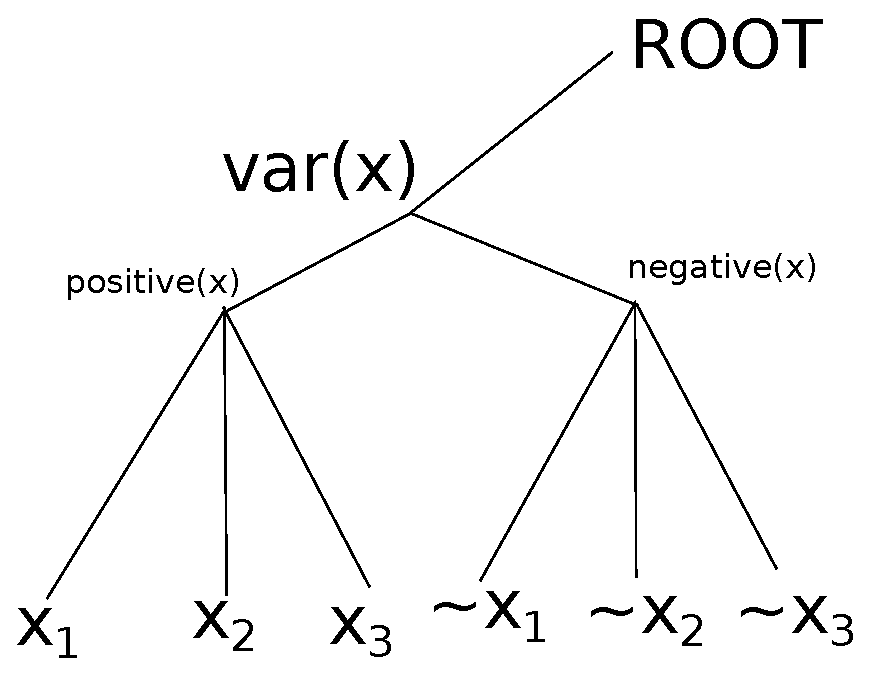
\includegraphics[width = \columnwidth]{figs/gadget-no-bw}
\end{figure}


\begin{figure}[htbp]
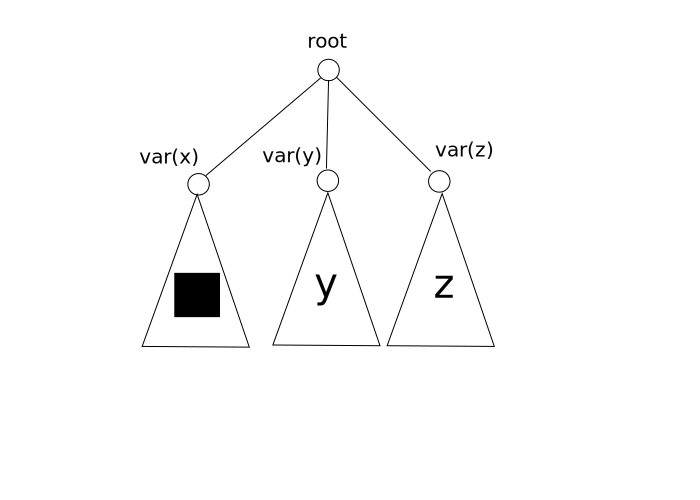
\includegraphics[width = \columnwidth]{figs/vc-instance}
\end{figure}


\begin{figure}[htbp]
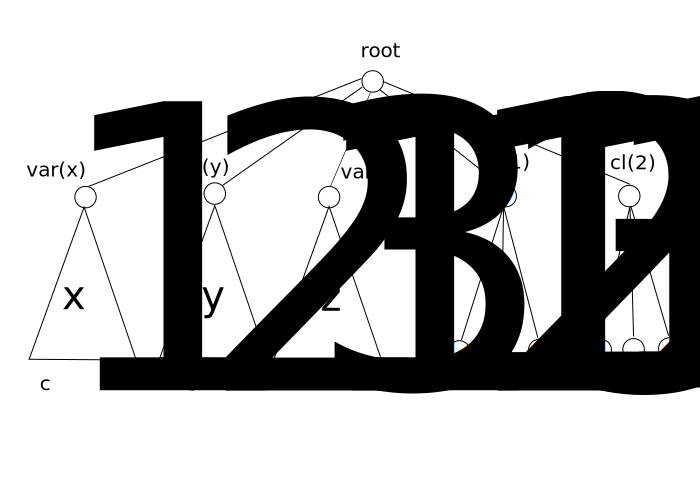
\includegraphics[width = \columnwidth]{figs/vc-instance-r2}
\end{figure}


\begin{figure}[htbp]
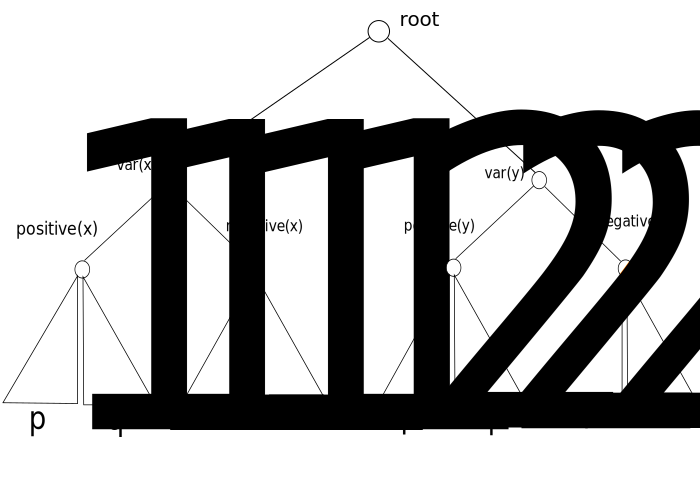
\includegraphics[width = \columnwidth]{figs/lemma-two-gadgets}
\end{figure}


\begin{figure}[htbp]
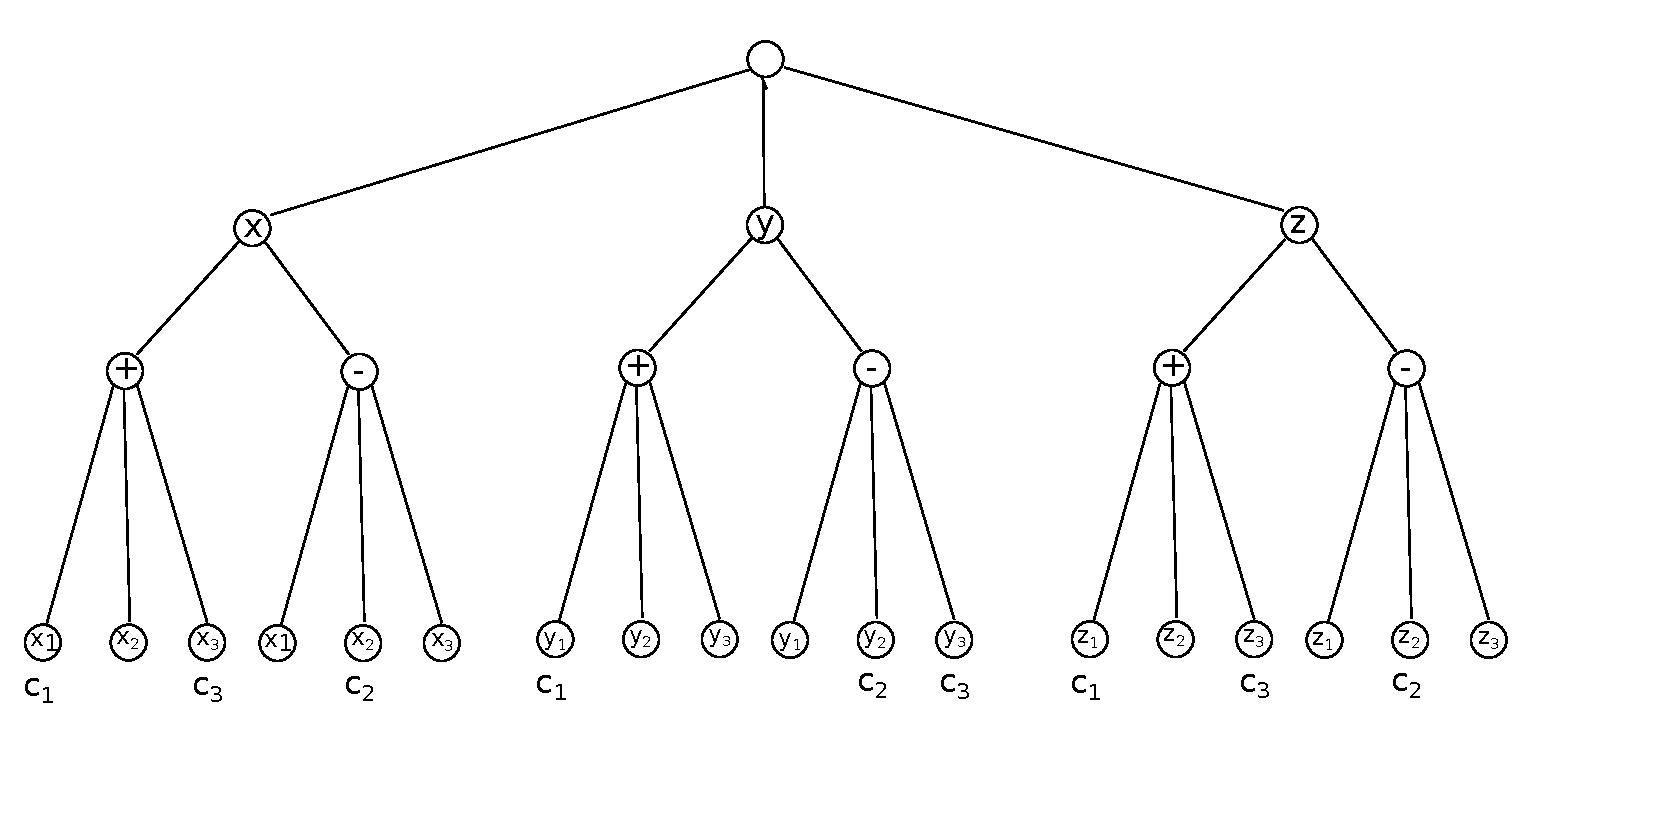
\includegraphics[width = \columnwidth]{figs/formula-example}
\end{figure}


\begin{figure}

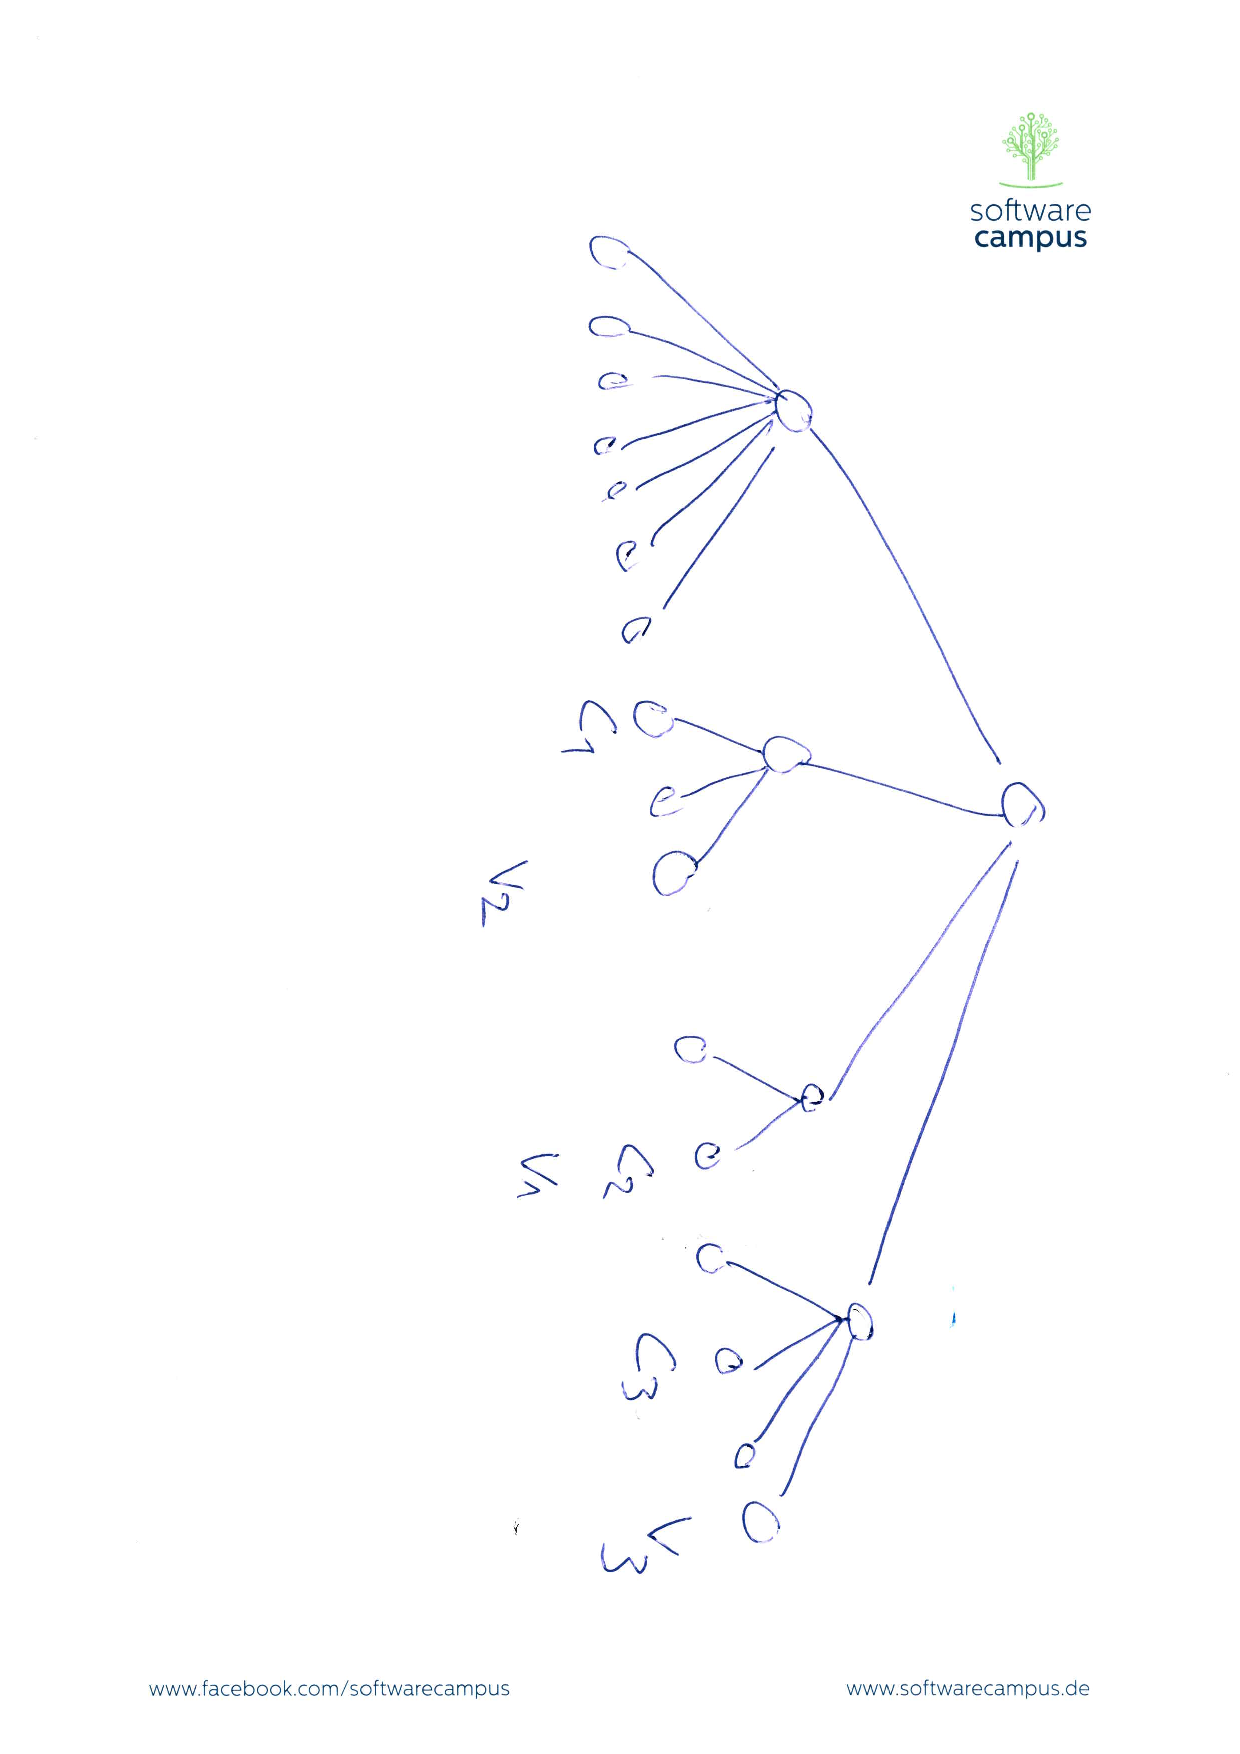
\includegraphics[angle=90,origin=c, height=7cm]{figs/model_fig_skteches/basic_problem}
\caption{basic problem}
\label{fig:basic_problem}
\end{figure}
\begin{figure}

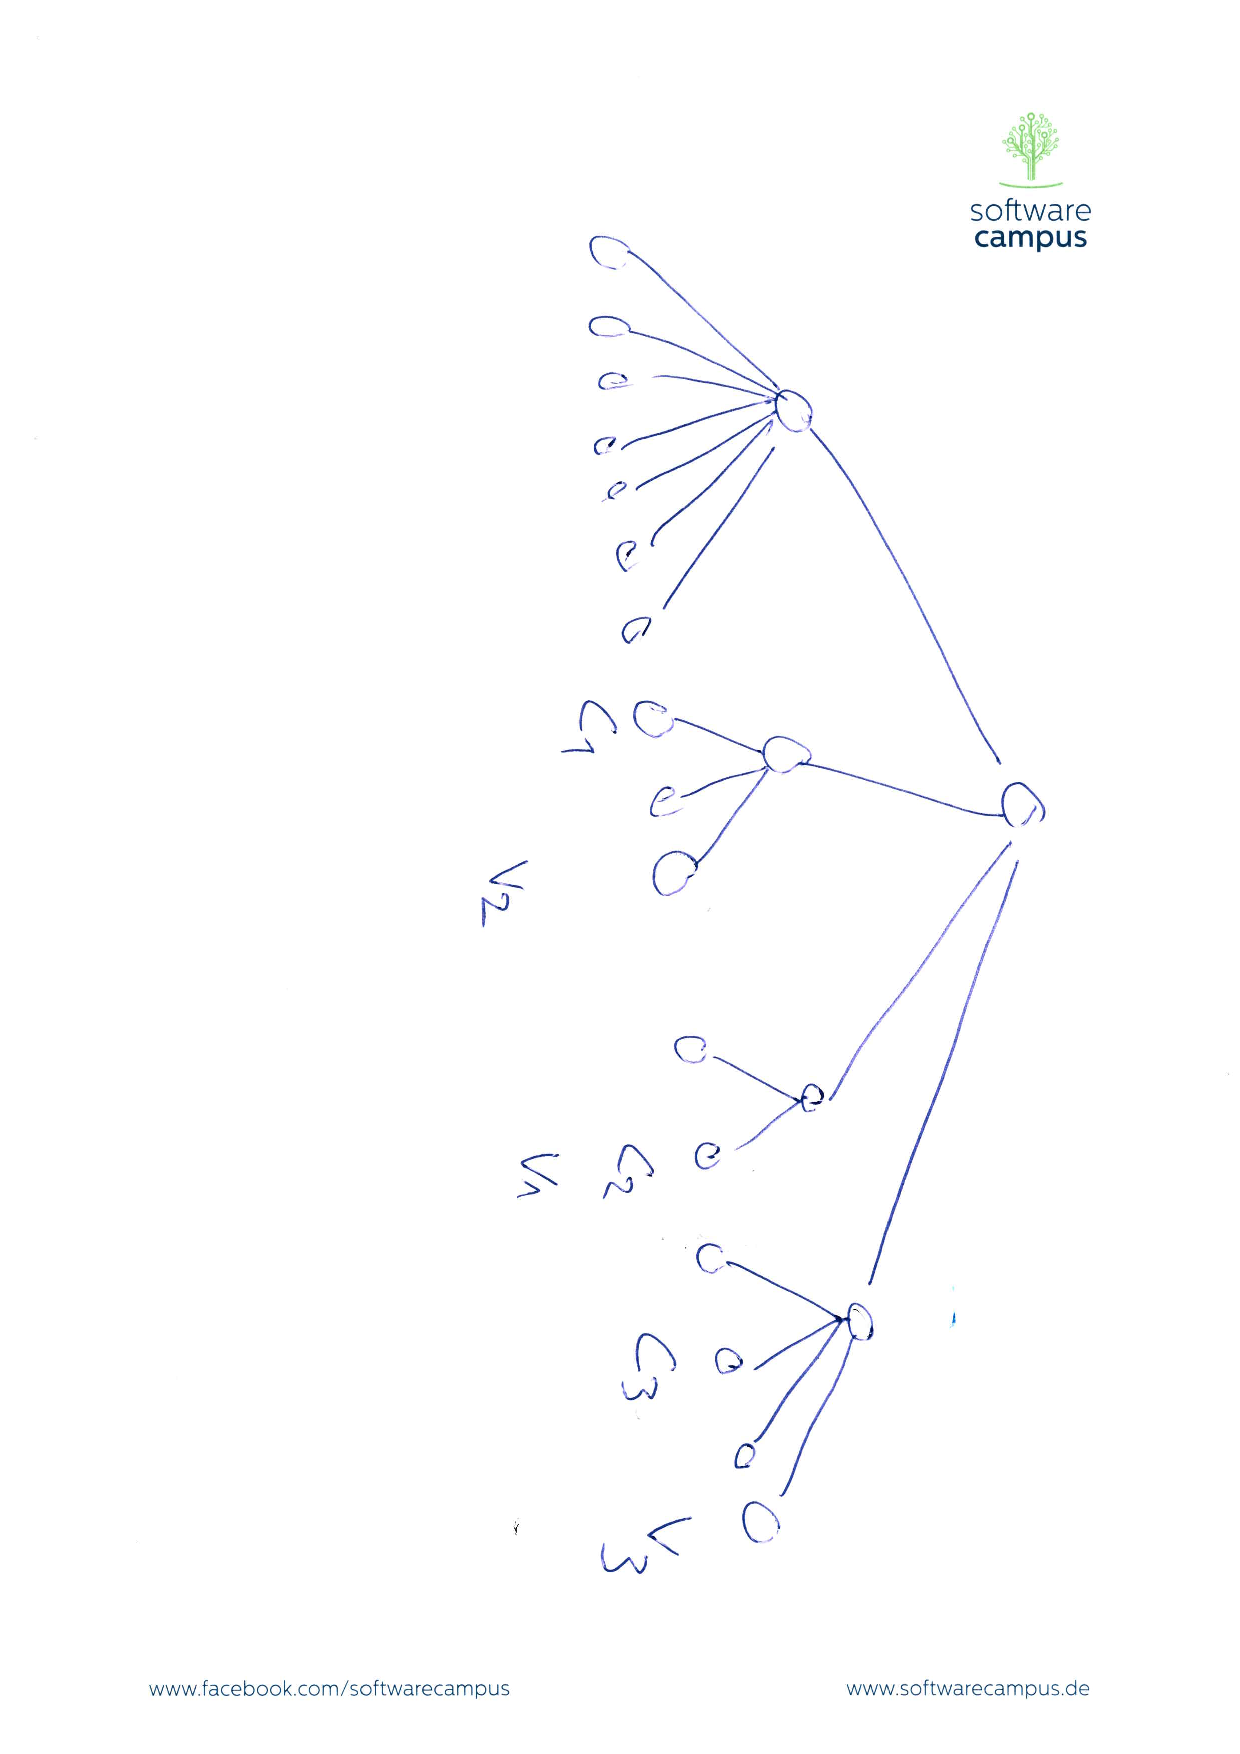
\includegraphics[angle=90,origin=c, height=7cm]{figs/model_fig_skteches/basic_problem}
\caption{solution for basic problem (green is pathes for transfer)}
\end{figure}

\begin{comment}

\section{Model}

This section describes our model. We will start by describing a simplistic
version of our model, and continue to introduce new properties until we reach
the full model.

\subsection{Symbols}

This is a dummy section to introduce the symbols used later...

\begin{description}
 \item [$\Tree$] the substrate tree with $\Tree = (\SubstrateNodes , \SubstrateEdges)$
 \item [$\SubstrateNodes$]  a set of nodes: $\{\SubstrateNode_1, \dots ,
\SubstrateNode_{|\SubstrateNodes|}\}$
 \item [$\SubstrateEdges$] a set of edges : $\{\SubstrateEdge_1, \dots ,
 \SubstrateEdge_{|\SubstrateEdge|}\}$ with $\SubstrateEdge_1 =
(\SubstrateNode_i, \SubstrateNode_j)$
 \item [$\achunk_i$] A chunk of type $i$
 \item [$v_i$] The i-th $\VM$ of the request
 \item [$\VirtualNodes$] the set of virtual Nodes = $\{1,2,\dots,\VCSwitch\}$
 \item [$\VirtualEdges$] the set of virtual Edges, $e_{V1}$ connects $1 \in
\VirtualNodes$ with $\VCSwitch \in \VirtualNodes$.
 \item [$\hat f$] the maximal flow
 \item [$|\hat f|$] the value of the maximal flow


 \item [$\Bandwidth$] Bandwidth constraint of an edge
 \item [$\CostTrans$] cost of chunk transport
 \item [$\CostCom$] cost of chunk communication
 \item [$\Vms$] number of VMs to spawn
 \item [$\ChunkTypes$] number of chunk types placed in an instance
 \item [$\Formula$] a formula
 \item [$\Clauses$] set of clauses in a formula
 \item [$\NClauses$] number of clauses in a given formula
 \item [$\Vars$] set of variables in a given formula
 \item [$\NVars$] number of variables in a given formula
 \item [$\Thr$] threshold
 \item [$\VCB$] virtual cluster model with bandwith
 \item [$\VCNB$] virtual cluster model without bandwith
 \item [$\varx$] variable
 \item [$\positive$] positive subtree of a gadget
 \item [$\negative$] negative subtree of a gadget
 \item [$\SAT$] set of satisfiable boolean formulas in CNF
 \item [$\TSAT$] set of satisfiable boolean formulas in 3CNF
 \item [$\Val$] valuation
 \item [$\Sol$] soultion to VC instance

\end{description}



\subsection{The Basic Model}

\carlo{Section TODO: How many / which figures + order?}

In the basic version of $\Problem$ data in the form of multiple chunks is
located in an undirected host graph tree $\Tree = (\SubstrateNodes,
\SubstrateEdges)$. A chunk $\achunk$ of the set of chunks $\Chunks =
\{\achunk_1,\dots,\achunk_{\ChunkTypes}\}$ can only be located at the leaves
$\Leaves = \{\Leaf_1,\dots,\Leaf_m\} \subset \SubstrateNodes$ of $\Tree$. We
denote the location of a chunk by $\ChunkLocation : \Chunks \rightarrow
\Leaves$. A cluster, consisting of a set of VMs $\VirtualNodes =
\{\VirtualNode_1,\dots,\VirtualNode_{\Vms}\}$, is allready embedded on the host
graph, and should process this data. The VMs are embedded on the
leaves of the tree, and we denote the location of the VMs by $\NodeMapping :
\VirtualNodes \rightarrow \Leaves$. We assume that $\Vms = \ChunkTypes$, each
VM $\VirtualNode_i$ can read the data of one chunk $\achunk_j$, and the data of
each chunk $\achunk_j \in \Chunks$ has to be processed. In order to process the
data from a chunk $\achunk_j$ with the VM $\VirtualNode_i$ it has to be
transferred along a (potentially empty) path $\Path_j =
\{\SubstrateEdge_{j_1},\dots,\SubstrateEdge_{j_n}\} ~ \SubstrateEdge_{j_k} \in
\SubstrateEdges$ such that $\SubstrateEdge_{j_1} = (\ChunkLocation(\achunk_j),
\SubstrateNode_x)$, $\SubstrateEdge_{j_k} = (\SubstrateNode_x,
\SubstrateNode_y) \rightarrow \SubstrateEdge_{j_{k+1}} = (\SubstrateNode_y ,
\SubstrateNode_z)$, and $\SubstrateEdge_n = (\SubstrateNode_y,
\NodeMapping(\VirtualNode_i))$.  For the sake of simplicity we assume that
transferring a chunk over a link in the host graph inflicts bandwidth cost of
$\CostTrans$ on this link. \carlo{NEW: We refer to the sum of all bandwidth
costs for the transport of specific chunks to vms by the function
$\CostPerChunk : \Chunks \cup \VirtualNodes \rightarrow \mathbb{R}$. Note, that
$\CostPerChunk(\achunk_j) = \CostPerChunk(\VmChunkAssignment(\achunk_j))$ and
$\CostPerChunk(\achunk_j) = \Distance(\ChunkLocation(\achunk_j),
\NodeMapping(\VmChunkAssignment(\achunk_j))) \cdot \CostTrans$, where $\Distance
: \SubstrateNodes \times \SubstrateNodes \rightarrow \mathbb{N}$ denotes the
distance in number of hops of two nodes in the host graph.} The overall
objective of $\Problem$ is to find an
assignment of VMs to chunks $\VmChunkAssignment : \Chunks \rightarrow
\SubstrateNodes$, so that the overall costs $\sum_{j \in
\{1,\dots,\ChunkTypes\}} |\Path_j|$ are minimized.

Throughout this section we will introduce different properties, to extend this
basic model. These properties can (and will) be combined to form more
challenging instances of $\Problem$.

%\begin{figure}[htbp]
%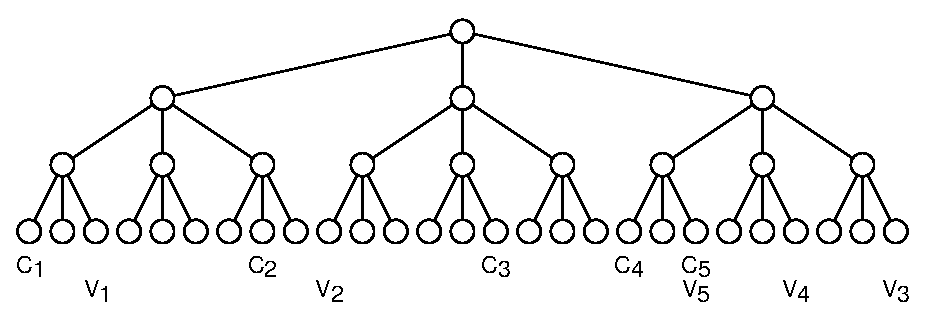
\includegraphics[width = \columnwidth]{figs/basic_scenario_3.eps}
%\caption{An example situation with 5 $\achunk s$ and $\VM s$. Note that $c_5$
%and $v_5$ are on the same host.}
%\label{fig:model_clean}
%\end{figure}
%
%
%
%Figure~\ref{fig:model_clean} shows an example situation with $n = 5$. The goal
%of the $\Problem$  is to find an assignment of the $\VM s$ to the $\achunk s$,
%which minimizes the overall bandwidth consumption of the job.
%
%We will now exemplarically examine an assignment of $\achunk s$ to $\VM s$.
%Assume $c_1$ is assigned to $v_1$, $c2$ to $v2$, $c3$ to $v3$, $c4$ to $v4$
%and $c5$ to $v5$. Since $v_5$ runs on the same host, which contains $c_5$,
%transfering $c_5$ to $v_5$ will consume no bandwidth on the physical links.
%Hence we assume the overall bandwidth costs of the transfer to be $0$. The
%distrance between $v_1$ and $c_1$ is $2$ hops. Hence the transfer of the
%$\achunk$ to the $\VM$ will consume bandwidth on two links. As a result, the
%overall bandwidth costs is $2 \cdot b_t$, where $b_t$ is the bandwidth
%neccessary for the transfer of a $\achunk$. $v_4$ is $4$ hops away from $c_4$,
%which results in a total cost of $4 \cdot b_t$. Since the hop distance between
%$v_2$ and $c_2$ is 6, the costs for transferring the $\achunk$ is $6 \cdot
%b_t$. The same holds for $v_3$ and $c_3$. The overall bandwidth consumption of
%the assignment is hence $18 \cdot b_t$.
%
%This is not an optimal solution for the $\Problem$. To show this, we will
%inspect a similar mapping. The only difference in the optimal mapping, is that
%$v_3$ is assigned to $c_2$ and $v_2$ is assigned to $c_3$. The bandwidth costs
%for transfering $c_2$ to it's assigned $\VM$ do not change, since $v_3$ is
%still $6$ hops away. $c_3$ however is now only $4$ hops away from its assigned
%$\VM$, which results in an overall bandwidth consumption of $16 \cdot b_t$.

\subsection{Communication Costs - $cv$}

\carlo{TODO: new symbol?}

This model extension assumes, that each VM  $\VirtualNode_i \in \VirtualNodes$
has to communicate with each other VM $\VirtualNode_{j \neq i} \in
\VirtualNodes$. Hence, the virtual cluster, which is to be embedded on the
physical substrate no longer consists only of a set of VMs, but is extended by a
set of virtual edges $\VirtualEdges : \VirtualNodes \times \VirtualNodes$.
Similar to the transfer of the chunks to the VMs, these edges have to be mapped
to a path in the host graph, which connects the locations to which the two VMs
are mapped. For the sake of simplicity we assume, that two VMs which communicate
inflict bandwidth cost of $\CostCom$ on each link of the path, which they use
for their communication.

\carlo{NEW: With this model extension the total costs $\Cost = \Cost_T +
\Cost_C$ are composed of the costs for the transport $\Cost_T$ and the costs
for communication among the VMs $\Cost_C$. $\Cost_C$ depends only on
$\NodeMapping$, while $\Cost_T$ depends on $\NodeMapping$ and
$\VmChunkAssignment$.}

\begin{figure}

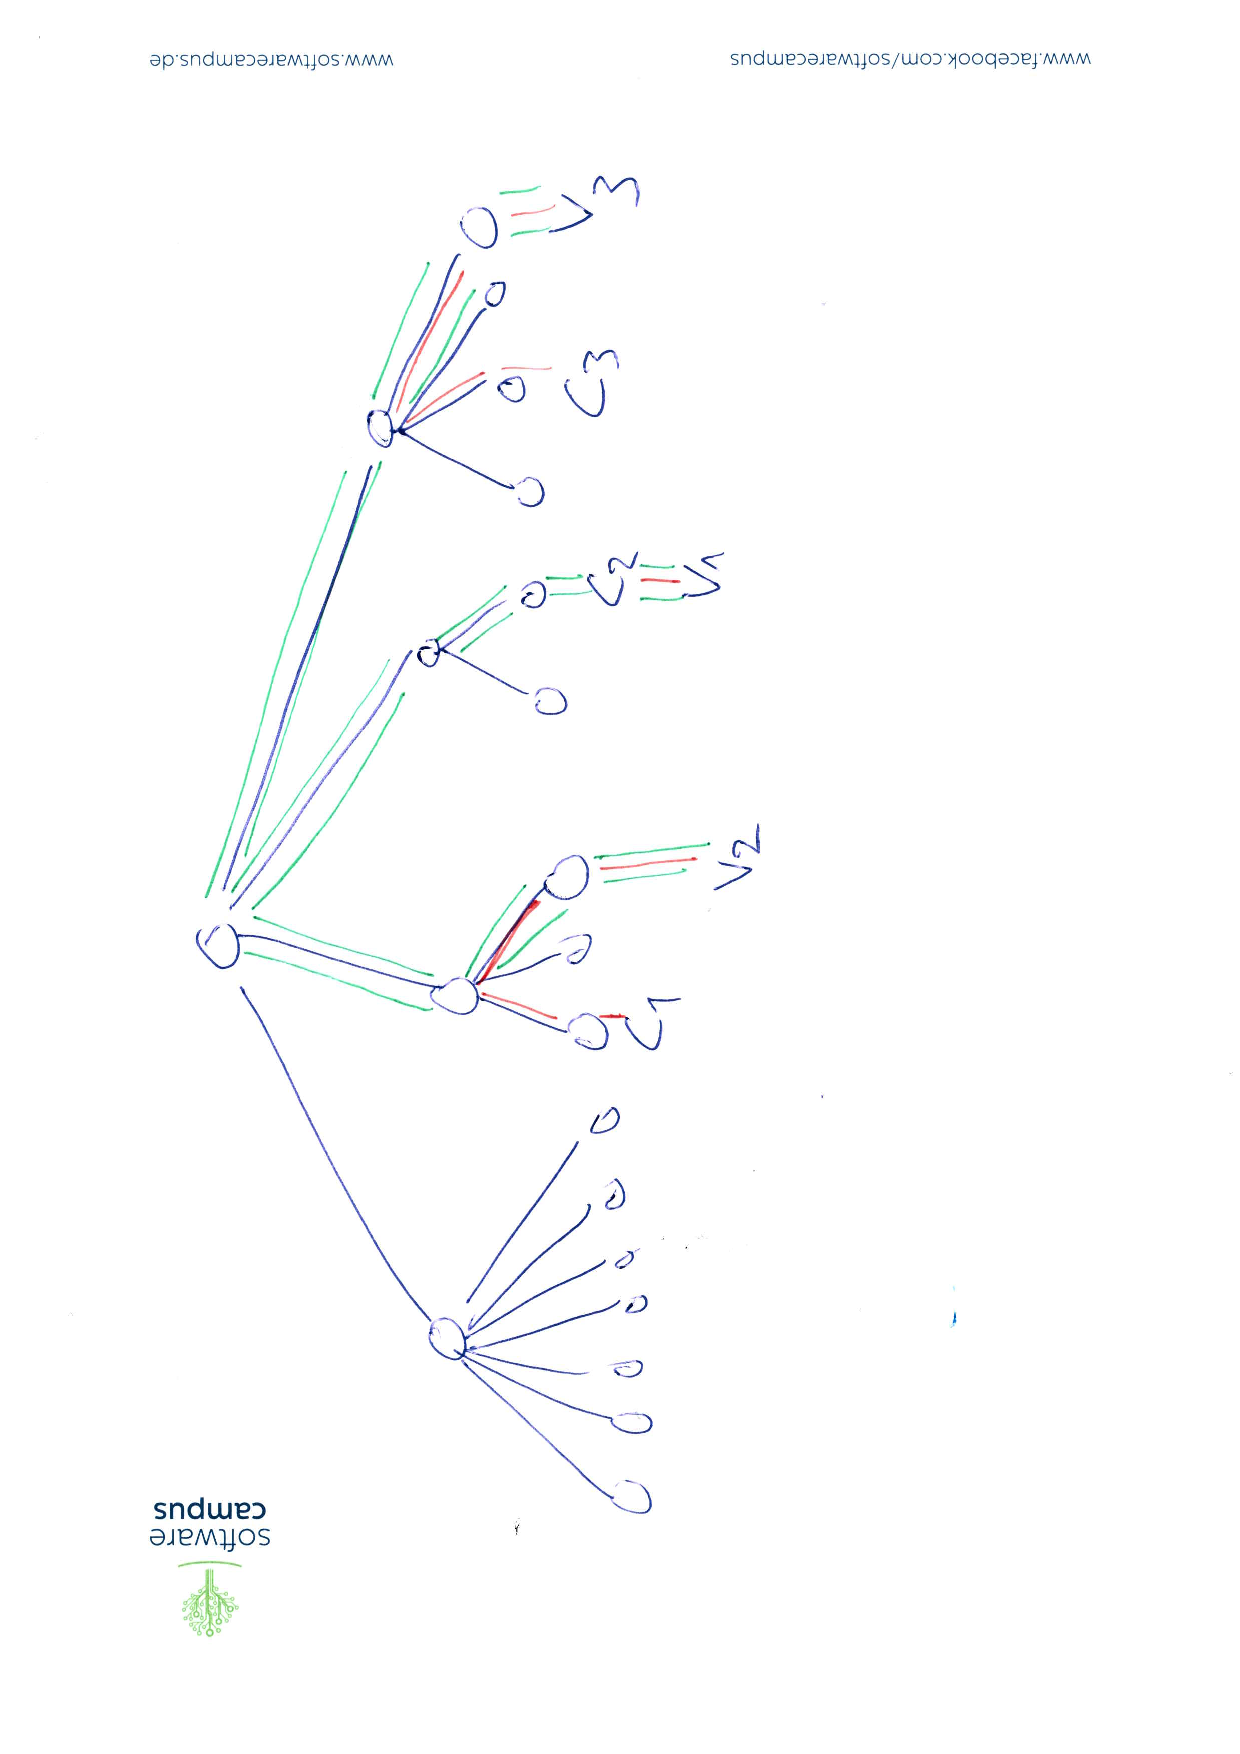
\includegraphics[angle=270,origin=c, height=7cm]{figs/model_fig_skteches/cv}
\caption{solution for problem with cv}
\end{figure}

%So
%far our model accounted bandwidth which is consumed to transfer data from it's
%location in the physical topology to the $\VM$ which will process it. However,
%due to the nature of distributed jobs, the $\VM s$ will also comunicate with
%each other. While we denoted the costs of transfering a chunk over a (1-hop)
%link with $b_t$, we will refer to the bandwidth costs of transfering data
%between a pair of $\VM s$ with $b_c$.


\subsection{Redundant Chunks - $r$}

This property specifies that, instead of having a single chunk $\achunk_j$, we
have $\RedundancyFactor$ redundant copies of each chunk
$\achunk_{j_1},\dots,\achunk_{j_\RedundancyFactor}  \in \Chunks$. These copies are
entirely equal, and only one instance of a specific chunk type (e.g.
$\achunk_{j_2}$) has to be read by one VM $\VirtualNode_j \in \VirtualNodes$.
Note that we assume chunks to be atomic - they cannot be read from two different
locations, requiering only $\CostTrans / 2$  bandwidth.

\begin{figure}

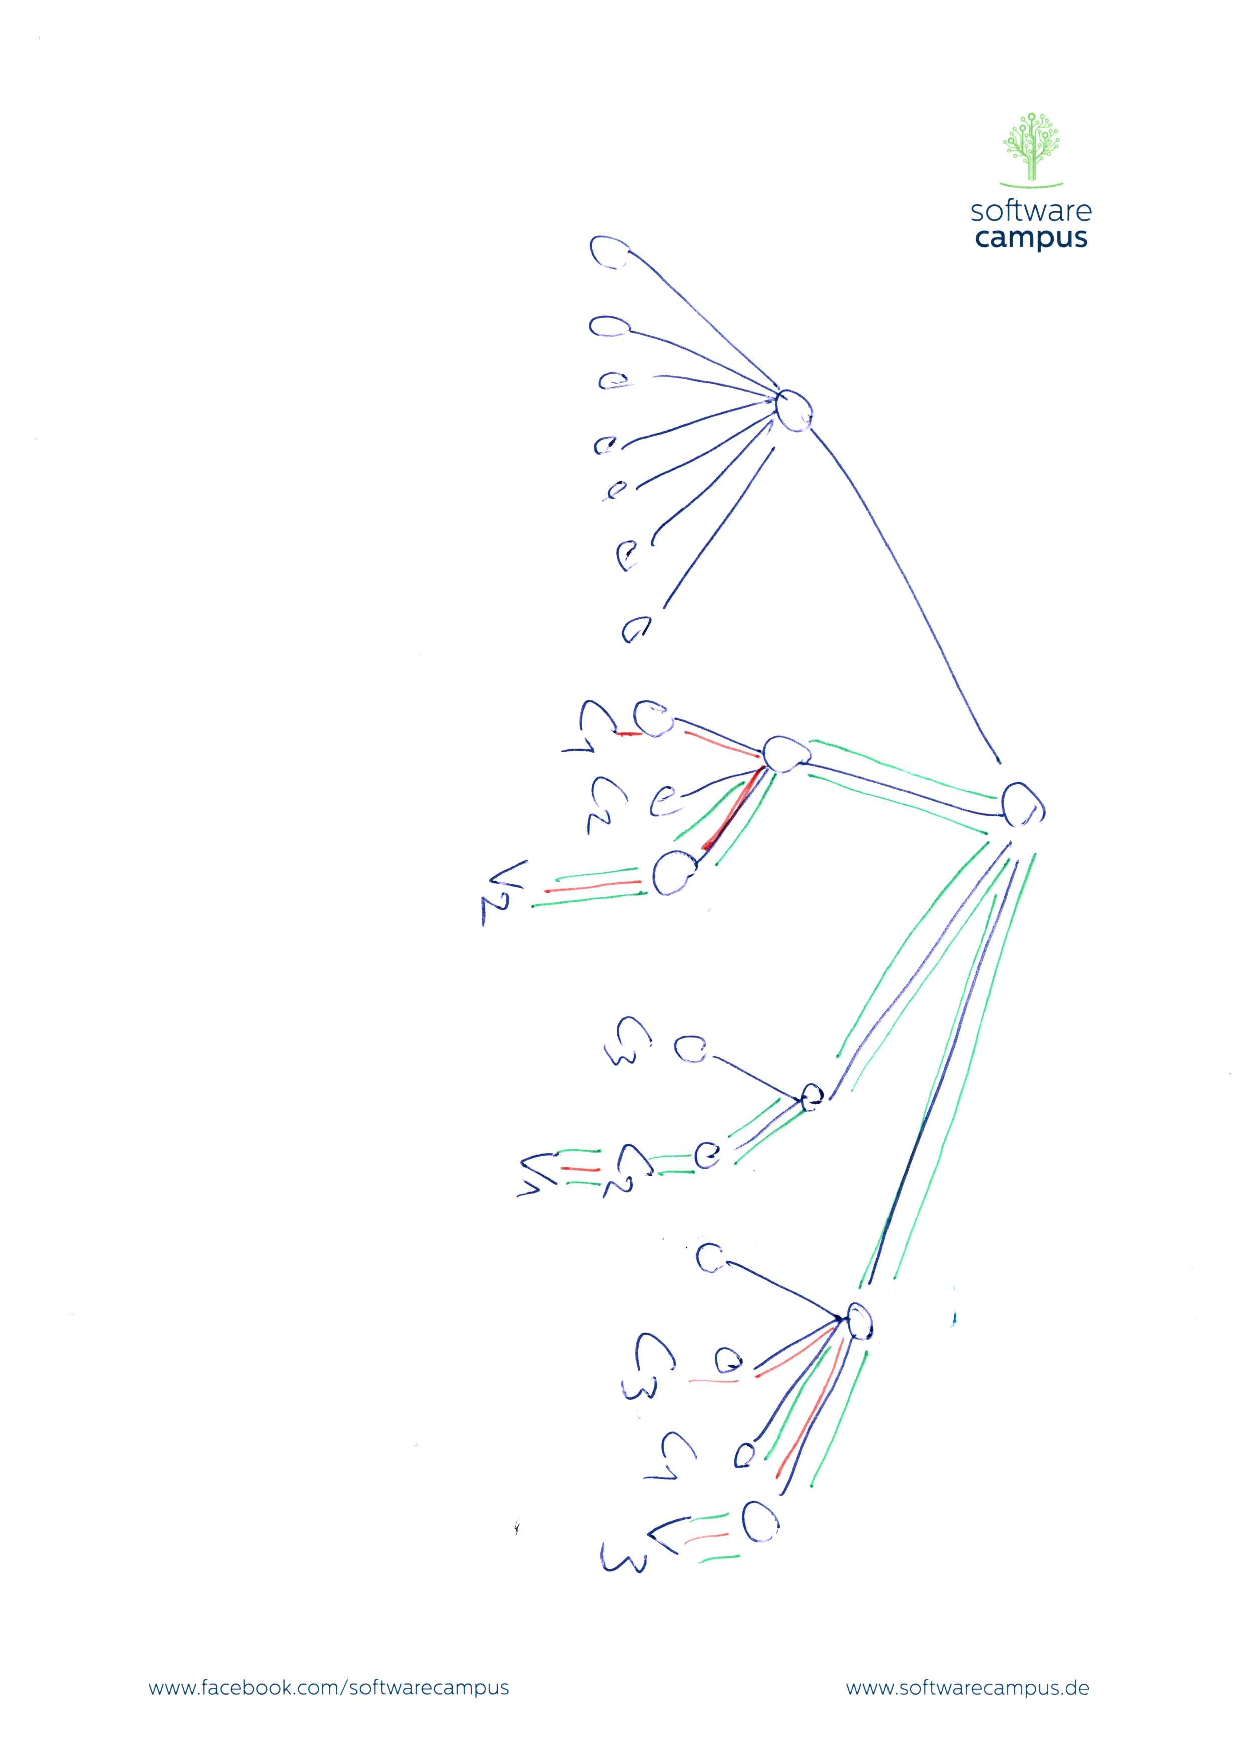
\includegraphics[angle=90,origin=c, height=7cm]{figs/model_fig_skteches/r_cv}
\caption{solution for problem with r}
\end{figure}




\subsection{Multiple Chunks per VM - $ma$}

This extension increases the processing capacities of the VMs. Instead of the
basic 1:1 ratio of VMs and chunks, this extension allows a VM to have $\MaFactor
\in \mathbb{N}^+$ many $\VmSlots$, which can all process chunks. We assume,
that the data which has to
be transferred to the VM from the chunks cannot be aggregated, and $\Vms =
\ChunkTypes / \MaFactor$.

\begin{figure}

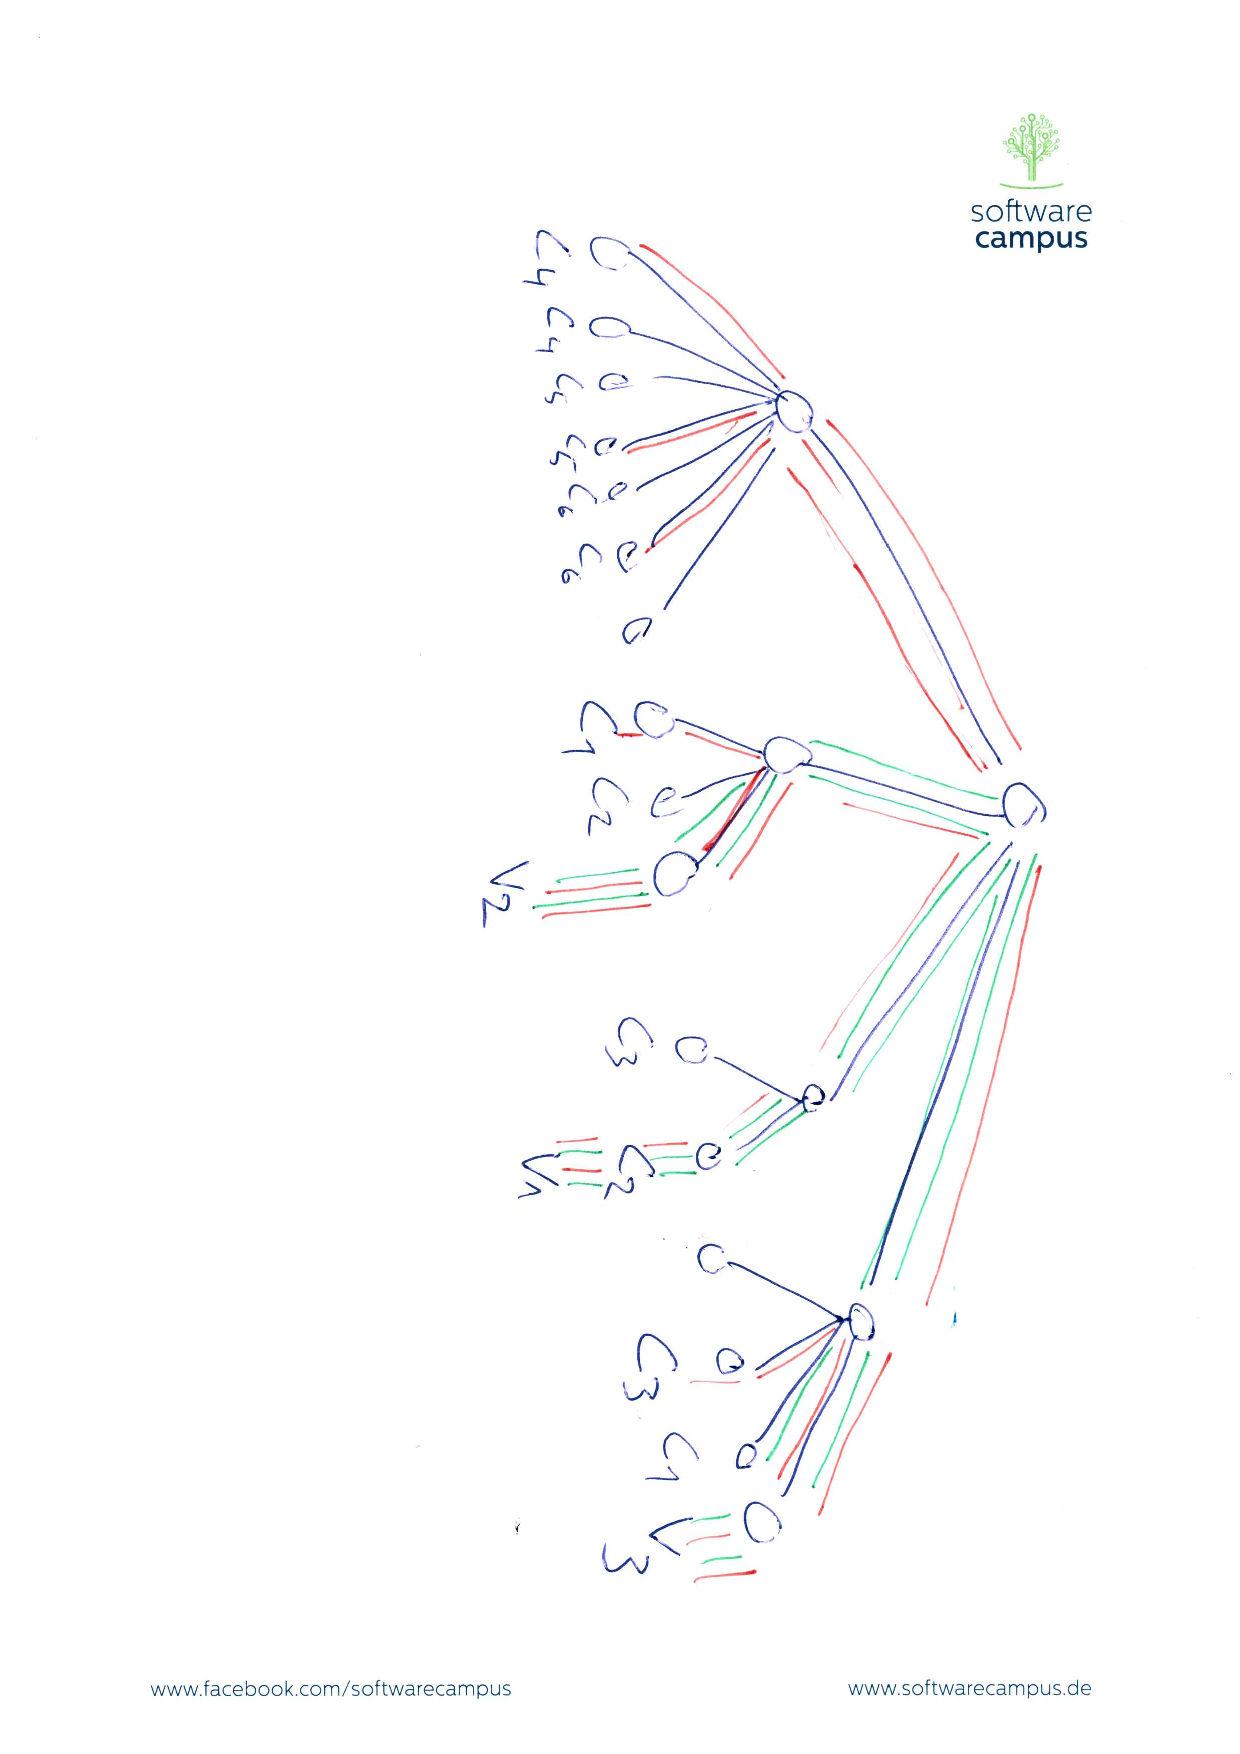
\includegraphics[angle=90,origin=c, height=7cm]{figs/model_fig_skteches/ma_r_cv}
\caption{soltion with ma}
\end{figure}

\subsection{Bandwidth Constraints - $bw$}

So far we only focussed on computing minimal bandwidth costs. However, in
reality the bandwidth which a single link can offer is limited. This model
extension limits the available bandwidth on each link $\SubstrateEdge_i \in
\SubstrateEdges$ in the host graph $\Tree$. We denote the capacity limitations
by $\Capacity : \SubstrateEdges \rightarrow \mathbb{R}$. The sum of all
bandwidth costs on this link, may never exeed it's capacity. Be aware that
this extension introduces infeasible instances.

\begin{figure}

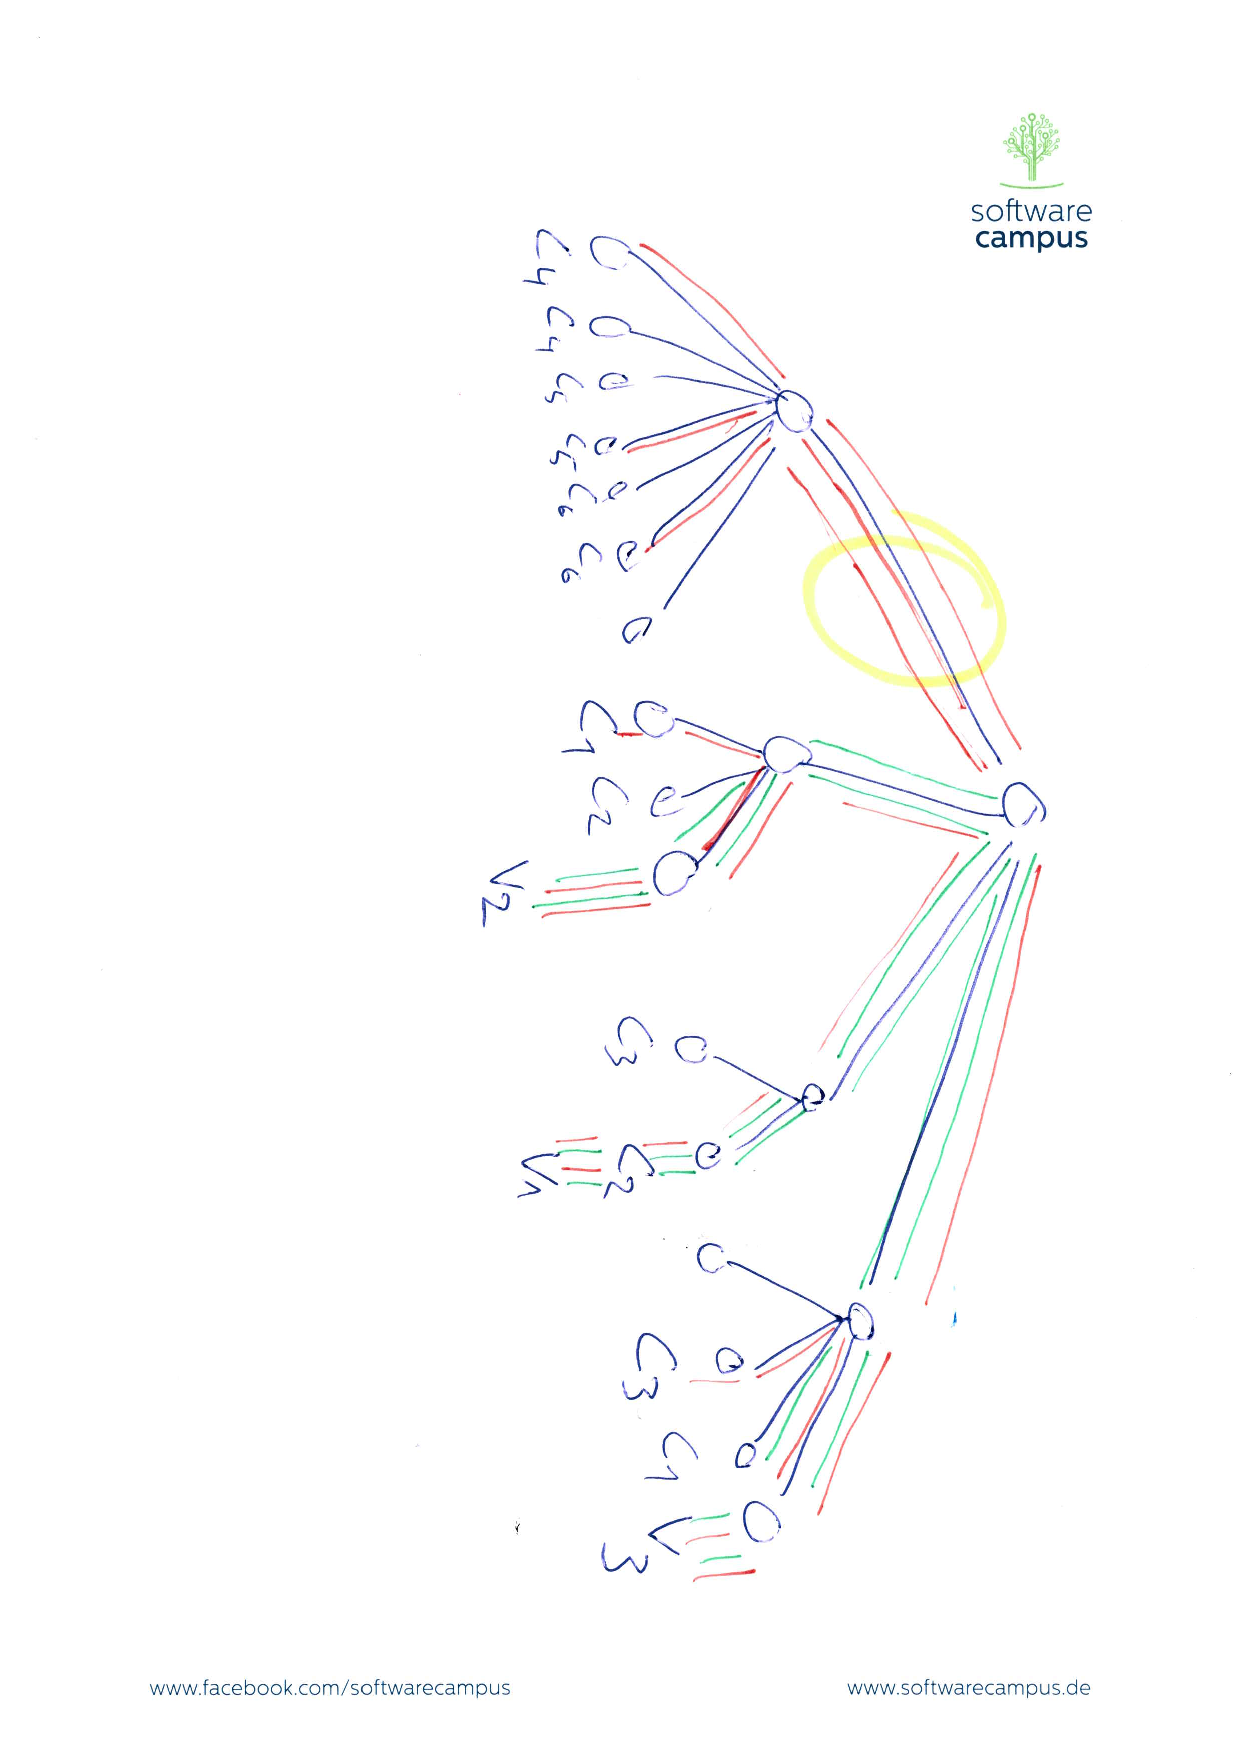
\includegraphics[angle=90,origin=c, height=7cm]{figs/model_fig_skteches/bw_ma_r_cv}
\caption{The bandwidth exceeds the capacity - independent of the chosen assignment}
\end{figure}
\subsection{Free VM Placement}

\begin{algorithm}[tbhp]
\DontPrintSemicolon % Some LaTeX compilers require you to use
%\dontprintsemicolon instead
\SetAlgoNoEnd
\KwIn{$\SubstrateNode \in \SubstrateNodes$}
\vspace{6pt}
\While{$|\Children(\SubstrateNode) > 2|$}{
  \textbf{set} $\SubstrateNodes \gets \SubstrateNodes \cup
\{\SubstrateNode^*\}$\;
  \textbf{~~with }$\Capacity(\SubstrateNode^*) \gets 0$
  \textbf{ and }$\Cost(\SubstrateNode^*) \gets  1$\;
  \textbf{choose any }$\SubstrateNode'$\textbf{ from
}$\Children(\SubstrateNode)$\;
  $cap \gets \Capacity((\SubstrateNode, \SubstrateNode'))$\;
  $\SubstrateEdges \gets \SubstrateEdges \setminus \{(\SubstrateNode,
\SubstrateNode')\}$\;
  \textbf{set} $\SubstrateEdges \gets \SubstrateEdges \cup \{(\SubstrateNode^*,
\SubstrateNode')\}$\;
  \textbf{~~with }$\Capacity((\SubstrateNode^*, \SubstrateNode')) i\gets cap$
  \textbf{ and }$\Cost((\SubstrateNode^*,\SubstrateNode')) \gets  1$\;
  \textbf{set} $\SubstrateNodes \gets \SubstrateNodes \cup \{(\SubstrateNode^*,
\SubstrateNode)\}$\;
  \textbf{~~with }$\Capacity((\SubstrateNode^*, \SubstrateNode)) i\gets \infty$
  \textbf{ and }$\Cost((\SubstrateNode^*, \SubstrateNode)) \gets  0$\;
  $binarize(\SubstrateNode')$\;
}
\For{\textbf{each } $\SubstrateNode' \in \Children(\SubstrateNode)$}{
  $binarize(\SubstrateNode')$\;
}

\caption{$binarize(\SubstrateNode \in \SubstrateNodes)$}
\label{algo:binarization}
\end{algorithm}


The Free VM Placement property describes a variant of our simple model, where
the positions of the VMs are not given in the problem statement but are
rather chosen by the described strategy. Concretely, $\NodeMapping$ is no
longer given, but part of the optimization within $\Problem$. We assume that
each leaf can only host one VM.

\subsection{Combined models} In this paper we analyse combinations of the
different properties listed above.

\begin{figure}[htbp]
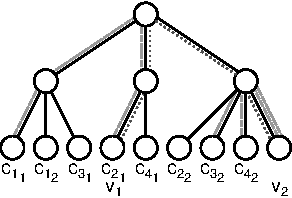
\includegraphics[width =\columnwidth]{figs/model_ma_r_cv}
\caption{An example instance of $\Problem$ with $ma$ + $cv$ + $r$. An
optimal solution is indicated by the dashed (transport costs) and dotted
(communication costs) lines. }
\label{fig:model_combined}
\end{figure}

An example of this can be seen in Figure~\ref{fig:model_combined}, which shows
an instance of $\Problem$, with the additional properties $ma$, $cv$ and $r$.
The host graph consists of 14 nodes. 9 nodes are leaves; 2 VMs are allready
embedded on leaves; with $\RedundancyFactor = 2$ and $\MaFactor = 2$ we have 4
chunk types, and two VMs of each type. The solution to this instance is also
depicted: The data from $\achunk_{1_1}$ and $\achunk_{2_1}$ is read by
$\VirtualNode_1$, $\achunk_{3_2}$ and $\achunk_{4_2}$ are read by
$\VirtualNode_2$. The dashed light gray lines indicate transport
costs $\CostTrans$. Note that no bandwidth is neccessary to transport data from
$\achunk_{2_1}$ to $\VirtualNode_1$, since these are collocated. The link
connecting the node, which hosts $\VirtualNode_2$ with it's parent, the
transport costs ammount to $2 \CostTrans$ - indicated by two dashed lines. In
addition to this, the figure illustrates the communication costs $\CostCom$,
which are indicated by the dotted dark gray line.

%\subsection{Summary of our results}

\begin{figure}[htbp]
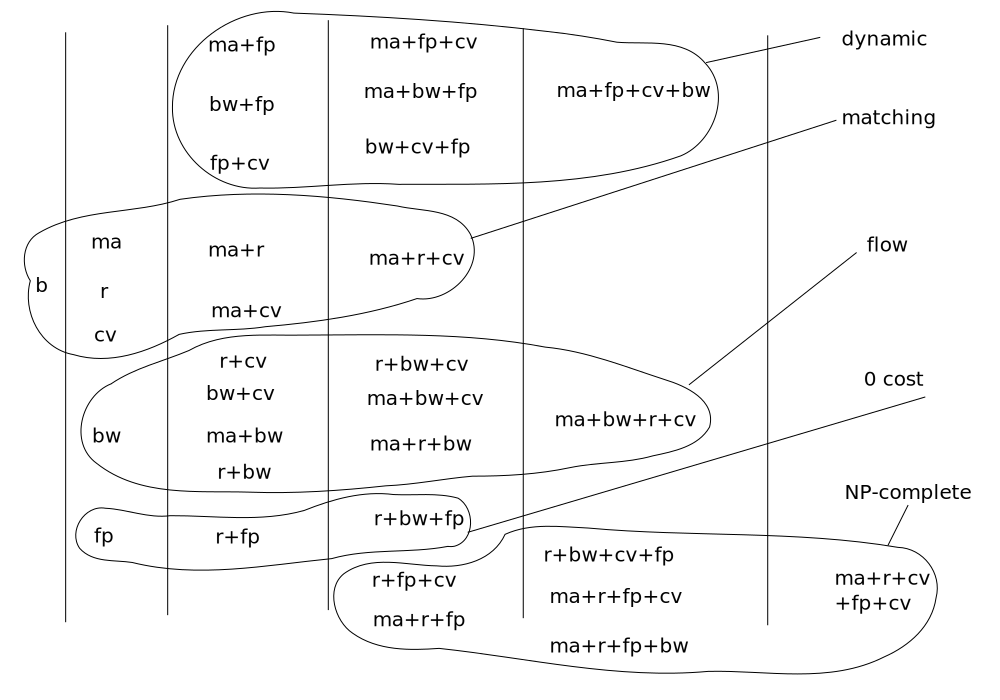
\includegraphics[width = \columnwidth]{figs/summary}
\caption{foo}
\label{fig:summary}
\end{figure}

This paper presents polynomial time algorithms or NP-hardness prooves for
\textit{all} possible comibnations of properties. An overview, of which problem
can be solved by which algorihms can be found in Figure~\ref{fig:summary}.

\begin{comment}
\begin{enumerate}
\item basic problem - M
\item ma - M
\item r - M
\item cv - reduces to basic problem
\item bw - F
\item fp - solution of 0 cost
\item ma + r - M
\item  ma + bw - F
\item ma + cv - reduces to ma
\item ma + fp - D
\item r + bw - F
\item r + cv - reduces to r
\item r + fp - solution of 0 cost
\item bw + cv - reduces to bw
\item bw + fp - D
\item fp + cv - D
\item ma + r + bw - F
\item ma + r + cv - reduces to ma + r
\item ma + r + fp - N
\item ma + bw + cv - reduces to ma + bw
\item ma + bw + fp - D
\item ma + fp + cv - D
\item r + bw + cv - reduces to r + bw
\item r + cv + fp - N
\item r + bw + fp - solution of 0 cost
\item bw + cv + fp - D
\item ma + r + bw + cv - reduces to ma + r + bw
\item ma + r + bw + fp - N
\item ma + r + cv + fp - N
\item ma + fp + cv + bw - D
\item r + bw + cv + fp - N
\item ma + r + bw + cv + fp - N
\end{enumerate}

\subsection{Leftovers from dynamic program}
For the simplified computation, we first represent the substrate network
$\Tree$ in a different way: concretely, we \emph{binarize} $\Tree$.

Algorithm~\ref{algo:binarization}
shows the algorithm to recursively binarize a (sub-)tree with the root $v$:
%To binarize tree $\Tree$, we start by processing each vertex $v \in
%\SubstrateNodes$ in the following root to leaf manner:
While $v$ has more than
$2$ children, we choose an arbitrary node $v' \in \Children(v)$
and create a new virtual node $v^*$. We remove the edge $e = (v, v')$ which
connected $v$ to it's child $v'$ from $\SubstrateEdges$. Subsequently we create
a new edge, which connects the
child to the new node $e^*_1 = (v', v^*)$, set it's
$\Cost(e^*_1) = 1$ and it's capacity to the value of the removed edge $e$
($\Capacity(e^*_1) = \Capacity(e)$). Additionally we generate an edge $e^*_2 =
(v^*, v)$. $\Capacity(e^*_2)$ is $\infty$ and $\Cost{e^*_2}$ is set to $0$.
Subsequently we process the subtree with the root $v'$. If the current node has
two or less children $v$ does not violate the binary constraint, and hence the
binarization process of $v$ is finished. However, it is necessary to
recursively binarize the subtrees with roots $v'_1, v'_2 \in \Children(v)$, if
they exists.
\newcommand{\NodesToProcess}{\ensuremath{\textsc{nodesToProcess}}}

\begin{algorithm}[tbhp]
\DontPrintSemicolon % Some LaTeX compilers require you to use
%\dontprintsemicolon instead
\SetAlgoNoEnd
\KwIn{$\SubstrateNode \in \SubstrateNodes$}
\vspace{6pt}
\While{$|\Children(\SubstrateNode) > 2|$}{
  \textbf{set} $\SubstrateNodes \gets \SubstrateNodes \cup
\{\SubstrateNode^*\}$\;
  \textbf{~~with }$\Capacity(\SubstrateNode^*) \gets 0$
  \textbf{ and }$\Cost(\SubstrateNode^*) \gets  1$\;
  \textbf{choose any }$\SubstrateNode'$\textbf{ from
}$\Children(\SubstrateNode)$\;
  $cap \gets \Capacity((\SubstrateNode, \SubstrateNode'))$\;
  $\SubstrateEdges \gets \SubstrateEdges \setminus \{(\SubstrateNode,
\SubstrateNode')\}$\;
  \textbf{set} $\SubstrateEdges \gets \SubstrateEdges \cup \{(\SubstrateNode^*,
\SubstrateNode')\}$\;
  \textbf{~~with }$\Capacity((\SubstrateNode^*, \SubstrateNode')) i\gets cap$
  \textbf{ and }$\Cost((\SubstrateNode^*,\SubstrateNode')) \gets  1$\;
  \textbf{set} $\SubstrateNodes \gets \SubstrateNodes \cup \{(\SubstrateNode^*,
\SubstrateNode)\}$\;
  \textbf{~~with }$\Capacity((\SubstrateNode^*, \SubstrateNode)) i\gets \infty$
  \textbf{ and }$\Cost((\SubstrateNode^*, \SubstrateNode)) \gets  0$\;
  $binarize(\SubstrateNode')$\;
}
\For{\textbf{each } $\SubstrateNode' \in \Children(\SubstrateNode)$}{
  $binarize(\SubstrateNode')$\;
}

\caption{$binarize(\SubstrateNode \in \SubstrateNodes)$}
\label{algo:binarization}
\end{algorithm}


\section{Dynamic Programs ($\MA+\CC+\FP+\BW$)}

The very powerful algorithmic technique to solve our problems
is dynamic programming. In this section, a general algorithm
is presented which can deal both with flexible node placements
as well as with inter-connects between virtual machines as well
as bandwidth constraints.

In general, dynamic programming can be used for problems which have
the property that optimal solutions for smaller subproblems (which can be computed efficiently)
can be efficiently combined into solutions for larger subproblems.

For ease of presentation, we will first present an algorithm to solve
the problem $\FP+\CC$. Based on this algorithm, we will show how to extend
the approach to the $\MA+\CC+\FP+\BW$ problem, introducing $\MA$ and $\BW$ separatly.

%\subsection{new}

The key insights of our algorithm is that, given the
number of nodes and chunks located in a certain  subtree $\Tree'$ of $\Tree$, the
costs of an optimal assignment $\VmChunkAssignment$ on
$\Uplink(\SubstrateNode')$, where $\SubstrateNode'$ is the root of $\Tree'$,
can be computed efficiently; this introduces a decoupling which can be exploited by the
dynamic program.

Let us introduce the
functions $\ChunkCount : \SubstrateNodes
\rightarrow
2^\Chunks$
and $\VmCount : \SubstrateNodes \rightarrow 2^{\VirtualNodes}$,
to compute the number of nodes and chunks in a given subtree $\Tree'$
of a given root. The functions can
easily be computed in a
bottom-up manner. \maciek{Function VMCount makes no sense as ``static'' function, as we do not know where VMs will be placed. Reader does not have enough insight into the algorithm to distinguish between those two functions. IMHO it is much better to remove VMCount from here and just use k, the function argument name as number of VMs in given subtree.}

% Stefan: I dont think we need this:
%: All leaf nodes $\Leaf_i$ are initialized with $\ChunkCount(\Leaf_i)
%= \{\achunk_j\}$ if a chunk is present at $\Leaf_i$ ($\exists ~ \achunk_j \in
%\Chunks : \ChunkLocation(\achunk_j) = \Leaf_i \Leftrightarrow
%\ChunkCount(\Leaf_i) = \{\achunk_j\}$), and with $\ChunkCount(\Leaf_i) =
%\emptyset$ otherwise ($\ChunkLocation(\achunk_j) \neq \Leaf_i \forall \achunk_j
%\in
%\Chunks \Leftrightarrow \ChunkCount(\Leaf_i) = \emptyset$). On every non-leaf
%node $\SubstrateNode_i \in \SubstrateNodes / \Leaves$, $\ChunkCount$ is equal
%to the union of the childrens' $\ChunkCount$s
%($\ChunkCount(\SubstrateNode_i)
%= \bigcup_{\SubstrateNode_k \in \Children{\SubstrateNode_i}}
%\ChunkCount(\SubstrateNode_k)$).

\subsubsection{Optimality of greedy local matching (version without MA)}

Let us first consider the simpler problem.
We first observe that an optimal solution will always
match chunks to nodes in small subtrees. Concretely,
we have the following cost property.

\maciek{This lemma is not what we meant by local matching lemma. Why we care only about uplink? We should care about cost of whole local matching.}

\begin{lemma}
\label{lemma:local_matching}
For a given node mapping $\NodeMapping$ and for any subtree $\Tree'$
of $\Tree$ rooted at $\SubstrateNode'$, containing $n$ chunks and $m$
nodes, the bandwidth costs of an optimal matching $\VmChunkAssignment$
from chunks to nodes on link $\Uplink(\SubstrateNode')$ is $|n
- m| \cdot \CostTrans$.
\end{lemma}
\begin{proof}
\stefan{this proof can be radically simplified.}

The proof is by case distinction. For both cases $|\ChunkCount(\SubstrateNode')| >
|\VmCount(\SubstrateNode')|$ and $|\ChunkCount(\SubstrateNode')| \leq
|\VmCount(\SubstrateNode')|$, we show that an optimal assignment
$\VmChunkAssignment$ is local, i.e., chunks are mapped to nodes in the
same subtree.

\textbf{Case $|\ChunkCount(\SubstrateNode')| \leq |\VmCount(\SubstrateNode')$:}
We show that for any node mapping $\NodeMapping$ and any subtree $\Tree'$ of $\Tree$
with root $\SubstrateNode'$, which contains at least one node per
chunk, an
optimal chunk to node assignment $\VmChunkAssignment$, cannot assign a chunk
to a nodeoutside of $\Tree'$ ($\VmChunkAssignment(\achunk_j) \in
\VmCount(\SubstrateNode')~ \forall \achunk_j \in \ChunkCount(\SubstrateNode')$).
 By contradiction. Assume $\VmChunkAssignment$ is an optimal chunk to node
assignment $\VmChunkAssignment$ with $\VmChunkAssignment(\achunk_j)
=\VirtualNode_l \notin \VmCount(\SubstrateNode')$. $\VmChunkAssignment$ assigns
the property for any subtree $\Tree'$. From $|\ChunkCount(\SubstrateNode')|
\geq
|\VmCount(\SubstrateNode')|$ follows that there is at least one
combination of
node
$\VirtualNode_m \in \VmCount(\SubstrateNode')$ and chunk $\achunk_k \notin
\ChunkCount(\SubstrateNode')$ with $\VmChunkAssignment(\achunk_k) =
\VirtualNode_m$. Let $\Tree''$ with the root $\SubstrateNode''$ denote the
smallest subtree of $\Tree$ with $\Tree' \subset \Tree'' \subseteq \Tree$ and
$\VirtualNode_l \in \VmCount(\SubstrateNode'')$. We will now show, that an
alternate assignment $\VmChunkAssignment'$ with
$\VmChunkAssignment'(\achunk_j) = \VirtualNode_m$ and
$\VmChunkAssignment'(\achunk_k) = \VirtualNode_l$, as lower costs, to generate
the contradiction. We do this, with the following case differentiation:
\textbf{Case 1:} $\achunk_k \in \ChunkCount(\SubstrateNode'')$\\
$\Distance(\NodeMapping(\VirtualNode_l), \ChunkLocation(\achunk_k)) \leq
\Distance(\NodeMapping(\VirtualNode_l), \ChunkLocation(\achunk_j)$ and
$\Distance(\NodeMapping(\VirtualNode_m), \ChunkLocation(\achunk_j)) <
\Distance(\NodeMapping(\VirtualNode_m), \ChunkLocation(\achunk_k)$. Due to the
direct correlation of $\CostPerChunk$ and $\Distance$, exchanging the
assignment of $\achunk_j$ and $\achunk_k$ will reduce the overall costs, since
$\CostPerChunk(\VirtualNode_m)$ will be reduced,
$\CostPerChunk(\VirtualNode_l)$ cannot be increased, and the other components
of the costs remain unchanged. As a result $\VmChunkAssignment'$ has lower
costs than $\VmChunkAssignment$, which is in contraction, to the optimality of
$\VmChunkAssignment$.\\
\textbf{Case 2:} $\achunk_k \notin \ChunkCount(\SubstrateNode'')$
Since $\Tree$ is balanced we get $\Distance(\NodeMapping(\VirtualNode_m),
\ChunkLocation(\achunk_k)  = \Distance(\NodeMapping(\VirtualNode_l),
\ChunkLocation(\achunk_k)$. In addition $\Distance(\NodeMapping(\VirtualNode_l,
\achunk_j)) > \Distance(\NodeMapping(\VirtualNode_m,
\achunk_j)) $ holds, since $\VirtualNode_m \in \VmCount(\SubstrateNode')$ and
$\VirtualNode_l \notin
\VmCount(\SubstrateNode')$. Hence swapping the assignment of $\achunk_j$ and
$\achunk_k$ will reduce $\CostPerChunk(\achunk_j)$, and keep all other costs
stable. This however is in contraction to the cost optimality of
$\VmChunkAssignment$, since $\VmChunkAssignment'$ would be cheaper.

\textbf{Case $|\ChunkCount(\SubstrateNode')| > |\VmCount(\SubstrateNode')$:}
For a given VM mapping $\NodeMapping$ and any subtree $\Tree'$ of $\Tree$
with the root $\SubstrateNode'$, which contains at least one chunk per
node $|\ChunkCount(\SubstrateNode')| \geq |\VmCount(\SubstrateNode')$, an
optimal chunk to node assignment $\VmChunkAssignment$, cannot assign a chunk
which is not in $\ChunkCount(\SubstrateNode')$ to a node in
$\VmCount(\SubstrateNode')$ ($\VmChunkAssignment(\achunk_j) \in
\VmCount(\SubstrateNode')~ \rightarrow \achunk_j \in
\ChunkCount(\SubstrateNode')$).
The proof is analogous to other one.
\end{proof}

If we also need to account for the cost of the inter-connect (the $\CC$ model),
the allocation of $\Uplink(\SubstrateNode')$ must be updated.

\stefan{I think we should include the following lemma also in the lemma above,
and make it one large (or hopefully not so large) theorem.}

\maciek{I do not understand at all what this lemma is about.}

\begin{lemma}
\label{lemma:comCost}
 For a given node mapping $\NodeMapping$ and any subtree $\Tree'$
 of $\Tree$ with the root $\SubstrateNode'$ with $n$ nodes,
 the allocation on
$\Uplink(\SubstrateNode')$ is $n \cdot (\Vms - n)
\cdot
\CostCom$.
\end{lemma}
\begin{proof}
As the node locations are given
and due to the tree property, the unique paths between
two nodes in the substrate do not contain
$\Uplink(\SubstrateNode')$ if both nodes are mapped to nodes in $\Tree'$.
However, each of the $n$ nodes inside $\Tree'$ has to communicate with each node
outside of $\Tree'$. The number of nodes outside $\Tree$ is the total number
of nodes, minus the amount of VMs inside $\Tree'$, resulting in $n \cdot (\Vms -
n)$ communications - which each inflict $\CostCom$ bandwidth costs.
\end{proof}

\subsubsection{Optimality of greedy local matching (version with MA)}

\begin{comment}

\stefan{I think we should maybe just discuss the differences here, not the entire thing again. Is this possible?
If not, we may even want to merge with the part above and nevertheless do it directly?}

\begin{lemma}
\label{lemma:adding-ma}
For a given node mapping $\NodeMapping$ and any subtree $\Tree'$
of $\Tree$ with root $\SubstrateNode'$ which contains $n$ chunks and $m$
nodes, the bandwidth costs of an optimal assignment $\VmChunkAssignment$ for
transferring the chunks to the nodes
on $\Uplink(\SubstrateNode')$ is $|n\cdot\MaFactor
- m| \cdot \CostTrans$.
\end{lemma}
\begin{proof}
\stefan{Also this proof we can simplify a lot.}


We can distinguish two cases:
$|\ChunkCount(\SubstrateNode')| \geq
|\VmCount(\SubstrateNode')| \cdot \MaFactor$ and
$|\ChunkCount(\SubstrateNode')| \leq
|\VmCount(\SubstrateNode')| \cdot \MaFactor$.
All chunks which cannot be served locally will be served in
other subtrees, resulting in the transport costs on $\Uplink(\SubstrateNode')$
described in Corollary~\ref{lemma:local_matching}. When the amount of
available $\VmSlots$
exceeds the amount of chunks in $\Tree'$, the transport costs will still occur,
since some chunks $\achunk_j \notin \ChunkCount(\SubstrateNode')$ will have to
be transported to the VMs in $\VmCount(\SubstrateNode')$, which have $\VmSlots$
which cannot be
assigned to chunks in $\ChunkCount(\SubstrateNode')$.

\textbf{Case at least one $\VmSlot$ per chunk:}
We show that for a given node mapping $\NodeMapping$ and any subtree $\Tree' \subseteq
\Tree$ with root $\SubstrateNode'$, which contains at least one $\VmSlot$
per
chunk $|\ChunkCount(\SubstrateNode')| \leq |\VmCount(\SubstrateNode')| \cdot
\MaFactor$, an
optimal chunk to VM assignment $\VmChunkAssignment$, cannot assign a chunk
to a VM outside of $\Tree'$ ($\VmChunkAssignment(\achunk_j) \in
\VmCount(\SubstrateNode')~ \forall \achunk_j \in \ChunkCount(\SubstrateNode')$).
The proof is by contradiction. Assume $\VmChunkAssignment$ is an optimal chunk to node
assignment $\VmChunkAssignment$ with $\VmChunkAssignment(\achunk_j)
=\VirtualNode_l \notin \VmCount(\SubstrateNode')$. $\VmChunkAssignment$ assigns
the property for any subtree $\Tree'$. From $|\ChunkCount(\SubstrateNode')|
\geq
|\VmCount(\SubstrateNode')| \cdot \MaFactor$ follows that there is at least one
combination of
node $\VirtualNode_m \in \VmCount(\SubstrateNode')$ and chunk $\achunk_k \notin
\ChunkCount(\SubstrateNode')$ with $\VmChunkAssignment(\achunk_k) =
\VirtualNode_m$. Let $\Tree''$ with the root $\SubstrateNode''$ denote the
smallest subtree of $\Tree$ with $\Tree' \subset \Tree'' \subseteq \Tree$ and
$\VirtualNode_l \in \VmCount(\SubstrateNode'')$. We will now show, that an
alternate assignment $\VmChunkAssignment'$ with
$\VmChunkAssignment'(\achunk_j) = \VirtualNode_m$ and
$\VmChunkAssignment'(\achunk_k) = \VirtualNode_l$, as lower costs, to generate
the contradiction. We do this, with the following case differentiation:
\textbf{Case 1:} $\achunk_k \in \ChunkCount(\SubstrateNode'')$\\
$\Distance(\NodeMapping(\VirtualNode_l), \ChunkLocation(\achunk_k)) \leq
\Distance(\NodeMapping(\VirtualNode_l), \ChunkLocation(\achunk_j)$ and
$\Distance(\NodeMapping(\VirtualNode_m), \ChunkLocation(\achunk_j)) <
\Distance(\NodeMapping(\VirtualNode_m), \ChunkLocation(\achunk_k)$. Due to the
direct correlation of $\CostPerChunk$ and $\Distance$, exchanging the
assignment of $\achunk_j$ and $\achunk_k$ will reduce the overall costs, since
$\CostPerChunk(\VirtualNode_m)$ will be reduced,
$\CostPerChunk(\VirtualNode_l)$ cannot be increased, and the other components
of the costs remain unchanged. As a result $\VmChunkAssignment'$ has lower
costs than $\VmChunkAssignment$, which is in contraction, to the optimality of
$\VmChunkAssignment$.
\textbf{Case 2:} $\achunk_k \notin \ChunkCount(\SubstrateNode'')$\\
Since $\Tree$ is balanced we get $\Distance(\NodeMapping(\VirtualNode_m),
\ChunkLocation(\achunk_k)  = \Distance(\NodeMapping(\VirtualNode_l),
\ChunkLocation(\achunk_k)$. In addition $\Distance(\NodeMapping(\VirtualNode_l,
\achunk_j)) > \Distance(\NodeMapping(\VirtualNode_m,
\achunk_j)) $ holds, since $\VirtualNode_m \in \VmCount(\SubstrateNode')$ and
$\VirtualNode_l \notin
\VmCount(\SubstrateNode')$. Hence swapping the assignment of $\achunk_j$ and
$\achunk_k$ will reduce $\CostPerChunk(\achunk_j)$, and keep all other costs
stable. This however is in contraction to the cost optimality of
$\VmChunkAssignment$, since $\VmChunkAssignment'$ would be cheaper.

\textbf{Case at least one chunk per $\VmSlot$:}
For a given VM mapping $\NodeMapping$ and any subtree $\Tree'$ of $\Tree$ with
root $\SubstrateNode'$, which contains at least one chunk per
$\VmSlot$ $|\ChunkCount(\SubstrateNode')| \geq |\VmCount(\SubstrateNode')|
\cdot \MaFactor$, an
optimal chunk to node assignment $\VmChunkAssignment$, cannot assign a chunk
which is not in $\ChunkCount(\SubstrateNode')$ to a node in
$\VmCount(\SubstrateNode')$ ($\VmChunkAssignment(\achunk_j) \in
\VmCount(\SubstrateNode')~ \rightarrow \achunk_j \in
\ChunkCount(\SubstrateNode')$).
 The proof is analog to above.
\stefan{We should at least combine the two proofs if possible.}
\end{proof}

If the $cv$ property is present in our model, transportation costs might not be
the only costs, which occur on $\Uplink(\SubstrateNode')$. The second cause of
bandwidth costs, are the inter VM communication cost $\Cost_C$.

\stefan{again, the following corollary is quite trivial, and we should maybe better make the whole
thing one big theorem, maybe with two lemmas in the proof, but maybe not even that.}

\begin{corollary}
\label{corollary:comCost}
 For a given VM mapping $\NodeMapping$ and any subtree $\Tree' \subseteq
\Tree$ with the root $\SubstrateNode'$, which contains $n
= |\VmCount(\SubstrateNode')|$ VMs, the communication costs ($\Cost_C$
component) on
$\Uplink(\SubstrateNode')$ are $n \cdot (\Vms - n)
\cdot
\CostCom$.
\end{corollary}

\begin{proof}
Due to the fact the nodemapping is given, the enpoints of the communication
pathes are known. Since $\Tree$ is a tree, there exists only one path between
two nodes in the substrate. These pathes do not contain the
$\Uplink(\SubstrateNode')$ if, both VMs are mapped to nodes in $\Tree'$.
However, each of the $n$ VMs inside $\Tree'$ has to communicate with each VM
outside of $\Tree'$. The number of VMs outside of $\Tree$ is the total number
of VMs, minus the amount of VMs inside $\Tree'$, resulting in $n \cdot (\Vms -
n)$ communications - which each inflict $\CostCom$ bandwidth costs.
\end{proof}

%$\ChunkCount_\SubstrateNode$ contains the
%number of chunks at
%or below
%$\SubstrateNode$ and $\Opt_\SubstrateNode[i]~i\in \{0,\dots,\Vms\}$ contains
%the
%total cost ($\CostCom$ + $\CostTrans$) for placing $i$ VMs at or beneath
%$\SubstrateNode$. These costs account for bandwidth costs on
%$\Uplink(\SubstrateNode)$. To denote that it is impossible to place $i$ VMs at
%or beneath $\SubstrateNode$, we set $\Opt_\SubstrateNode[i] = \infty$.
%
%, we generate a
%function $\ChunkCount : \SubstrateNode \rightarrow \mathbb{N}$ and second
\maciek{I commented out everything in this section as it is generalization of section above which is wrong.}

\subsubsection{The $\MA+\FP+\CC$ Algorithm}

\maciek{I removed BW}
\maciek{Just one sentence about binarization is enough. Rest should belong to appendix}

Having characterizes the locality of optimal solutions as well as the resulting
bandwidth allocations, we can now present our dynamic program.
As already mentioned, our dynamic program leverages optimal solutions to
subproblems.

\maciek{Here we should start by: (1) we will consider all possible number of VMs in every subtree and all possible placements of VMs
  (2) introduce cost charging model - additional cost of two edges on each level (3) symmetrical cost of difference of slots and chunks - it allows for creating incomplete transfer out of subtree (3) we can use optimal value for subtrees for constructing optimal value for tree (4) present the recursive formula (for FP+NI only) (5) present the complete algorithm, with base cases and aggregate function (6) say just one sentence about effective implementation (arrays) (7) reconstruction of solution from cost array (8) analyze the runtime}

To compute a solution $\Sol$ use a
function $\Opt : \SubstrateNodes \times \mathbb{N} \rightarrow \mathbb{R}$.
$\Opt$ represents the inflicted bandwidth costs in a subtree $\Tree'$ of $\Tree$
with root $\SubstrateNode'$, which will occur if $n$ (argument 2)
nodes, will be placed in $\Tree'$.
This
function can be evaluated
efficiently in a bottom up manner. After $\Opt$ is evaluated for the entire
tree, $\Sol$ can be constructed from the values of $\Opt$.
%If $|\Children(v)| > 2$, we choose an arbitrary node $v' \in \Children(v)$
%and create a new virtual node $v^*$. We create a new edge $e^*_1$, set it's
%cost to $1$ and it's capacity to $\Bandwidth(e)$.

%In addition we evaluate a function $\ChunkCount : \SubstrateNodes \rightarrow
%2^\Chunks$, which yields which chunks are located beneath a specific node in
%the host graph. The evaluation of $\ChunkCount$ can be done in a simple
%bottom
%up manner: All leaf nodes $\Leaf_i$ are initialized with
%\ChunkCount(\Leaf_i)
%= \{\achunk_j\}$ if a chunk is present at $\Leaf_i$ ($\exists ~ \achunk_j \in
%\Chunks : \ChunkLocation(\achunk_j) = \Leaf_i \Leftrightarrow
%\ChunkCount(\Leaf_i) = \{\achunk_j\}$.), and with $\ChunkCount(\Leaf_i) =
%\emptyset$ otherwise ($\ChunkLocation(\achunk_j) \neq \Leaf_i \forall \achunk
%\in
%\Chunks \Leftrightarrow \ChunkCount(\Leaf_i) = \emptyset$). On every non-leaf
%node $\SubstrateNode_i \in \SubstrateNodes / \Leaves$, the count count is
%equal
%to the union of the childrens chunk count values
%($\ChunkCount(\SubstrateNode_i)
%= \bigcup_{\SubstrateNode_k \in \Children{\SubstrateNode_i}}
%\ChunkCount(\SubstrateNode_k)$).
$\Opt$ is initialized at the leaves as follows:
Either zer or one nodes are mapped at the Leaf $\Leaf_i$,
and we set $\Opt(\Leaf_i, n \in
\{0,1\}) = 0$; for all other number of nodes we set $\Opt(\Leaf_i, n \in
\{2,\dots,\Vms\}) = \infty$ (infeasible due to capacity constraints).

To recursively compute $\Opt(\SubstrateNode_i, n \in \{0,\dots\Vms\})$ for a
non-leaf node $\SubstrateNode_i \in \SubstrateNodes / \Leaves$, we leverage
Corollaries~\ref{lemma:local_matching} and \ref{corollary:comCost}. Since
we do it in a bottom up manner, $\Opt(\SubstrateNode_c, n)$
is already evaluated for all $n \in \{0,\dots,\Vms\}$ and all
$\SubstrateNode_c \in \Children(\SubstrateNode_i)$.

Since nodes may only be embedded at leaves, the bandwidth costs of placing $n$ nodes
in the subtree $\SubstrateNode_i$ with the children $\SubstrateNode_l$ and
$\SubstrateNode_r$ can be divided into the costs of placing $l$ nodes in the
subtree with root $\SubstrateNode_l$, the costs of placing
$r$ VMs in the subtree with $\SubstrateNode_r$, and the costs on the
$\Uplink(\SubstrateNode_l)$ and $\Uplink(\SubstrateNode_r)$. The costs of
placing the VMs beneath the $\SubstrateNode_l$ are already known from
$\Opt$. \carlo{(New to put an emphasis on charging only two edges...:) The only
additional bandwidth costs on this level of recursion occur on
$\Uplink(\SubstrateNode_l)$ (and $\Uplink(\SubstrateNode_r)$ respectively).}
The costs on $\Uplink(\SubstrateNode_l)$ can again be divided: From
Corollary~\ref{lemma:local_matching}, we know that the transport costs are
 $|\ChunkCount(\SubstrateNode_l) - l| \cdot \CostTrans$ and from
Corollary\ref{corollary:comCost}, we know that the communication costs are
$l\cdot (\Vms - l) \cdot \CostCom$. The same is valid for $\SubstrateNode_r$.
We now iterate over all possible amounts of VMs $n \in \{0,\dots,\Vms\}$ and
try to find the cheapest split of $n$ into $\hat l$ and $\hat r$ with
$\hat l + \hat r = n$ for each $n$. We define $\Opt(\SubstrateNode_i, n) =
\Opt(\SubstrateNode_{l}, \hat l) + \Opt(\SubstrateNode_{r}, \hat r) +
(|\ChunkCount(\SubstrateNode_{l}) - \hat
l|+|\ChunkCount(\SubstrateNode_{r}) - \hat r|) \cdot \CostTrans + (\hat
l\cdot (\Vms - \hat l) + \hat r\cdot (\Vms - \hat r)) \cdot \CostCom$. If the
bandwidth sum on one of the uplinks exceeds the capacity defined by
$\Capacity$, we treat the solution as infeasible, by treating the costs as
$\infty$. Algorithm~\ref{algo:dynAggregation} illustrates this... \carlo{Do you
want to keep this?}

Since the total costs $\sum_{\achunk_j \in
\Chunks}\Cost(\achunk_j)$ of an optimal assignment $\VmChunkAssignment$
consists only of $\Cost_T$ and $\Cost_C$, for which $\Opt$ accounts accurately
(Corollaries~\ref{lemma:local_matching} and \ref{corollary:comCost}),
$\Opt(\SubstrateNode, \Vms)$ will be equal to $\sum_{\achunk_j \in
\Chunks}\Cost(\achunk_j)$ - or $\infty$ if the instance is infeasible.

\carlo{TODO Construction from $\Opt$ or described how to store? Or say trivial?}

\subsubsection{Implementation}

\begin{comment}
\carlo{I didn't know where you wanted to put this. Feel free to modify / move
it.}

An implementation of our DP based solution can be implemented efficiently,
using the following data structures: $\ChunkCount$ can be
represented by single values on the respective nodes in the host graph. The
node to which it is attached, will replace the argument of $\ChunkCount$: the
values will represent the amount of chunks, which are located in the subtree
with respective node, as root.

$\Opt$ can be realized by an array, which is attached to a node in the host
graph. The node again replaces the first argument. The index of the array, will
replace the second argument of $\Opt$. If a value in the array of node
$\SubstrateNode_i$ at index $i$ is set to a value $x$, this represents, that
placing $i$ VMs in the subtree beneath $\SubstrateNode_i$, will inflict
bandwidth costs of $x$ on the links in the subtree beneath $\SubstrateNode_i$.

Note that $\VmCount$ will not be implemented at all - it is only neccessary for
the former proofs.



\stefan{I dont think we really need this section:}
\maciek{I commented it out}

\subsubsection{Adding bandwidth constraints}

\maciek{I think that it is good to defer presenting bandwidth to this point and introduce it separatly. Also, lemma in this chapter is well-defined.}

\carlo{TODO: Move root to model section}

\begin{lemma}
An instance of $\Problem$ is infeasible if $\Opt(\SubstrateNode,\Vms) = \infty$,
where $\SubstrateNode$ is the root of $\Tree$.
\end{lemma}

\begin{proof}
By contraction: Assume the instance of $\Problem$ is feasible and
$\Opt(\SubstrateNode,\Vms) = \infty$. This menas a node mapping $\NodeMapping$
and an assignment $\VmChunkAssignment$ exists, which do not violate the
bandwidth capacities on all edges in $\SubstrateEdges$. Since VMs may only be
located at leaves, $\NodeMapping$ will place $r$ VMs in the subtree beneath the
right child of $\SubstrateNode$ and the remaining $\Vms - r$ VMs in the subtree
beneath the other child of $\SubstrateNode$.
$\Opt(\SubstrateNode,\Vms)$ can be $\infty$ due to two reasons, which can occur
at or beneath one of the children of $\SubstrateNode$. Let us without loss of
generality assume that the reason occured beneath the right child. The first
reason, is that there is not sufficient bandwidth
$\Capacity(\Uplink(\SubstrateNode_r)) < |\ChunkCount(\SubstrateNode_{r}) - r|)
\cdot \CostTrans + r \cdot (\Vms - r)) \cdot \CostCom$. From
Corollaries~\ref{lemma:local_matching} and~\ref{corollary:comCost} we know
that this contradicts the assumption that $\NodeMapping$
and $\VmChunkAssignment$ do not violate the bandwidth capacities
$\Uplink(\SubstrateNode_r)$. Hence the only reason why
$\Opt(\SubstrateNode,\Vms)$ can be $\infty$ is the second reason:
$\Opt(\SubstrateNode_r, r) = \infty$.

We can now repeat the same argumentation, showing that $\NodeMapping$ splits
the $r$ VMs which are located in the subtree beneath $\SubstrateNode_r$ in $r'$
and $l'$ VMs, which are located in the subtrees beneath the
children $\SubstrateNode_r$. The bandwidth argument is still valid on lower
layers, which will result in one of the children of $\SubstrateNode_r$ will
have a value of infinity for it's assigned amount of VMs. After some
recursive steps, this will result in $\Opt(\Leaf_j, \{0,1\}) = \infty$
for a leaf node - which have been initialized with $0$ and
are never modified.
\end{proof}

\end{comment}


\end{appendix}


\end{document}
